\documentclass[12pt,a4paper,twoside]{book}

% use Libertine font
\usepackage{libertine}
\usepackage{inconsolata}
\usepackage[T1]{fontenc}

\usepackage[utf8]{inputenc}
\usepackage[inline]{enumitem}
\usepackage{parskip} % disable indentation for new paragraphs, increased margin-bottom instead
\usepackage[main=american,ngerman]{babel}
\usepackage{csquotes}

\usepackage{kit_style/kitthesiscover}

\usepackage[style=numeric,backend=biber]{biblatex}
\addbibresource{bib.bib}
\addbibresource{bib_manual.bib}
\setcounter{biburlnumpenalty}{100}
\setcounter{biburllcpenalty}{7000}
\setcounter{biburlucpenalty}{8000}

\usepackage{todonotes}
\usepackage{blindtext}

\usepackage{xparse}

\usepackage{xspace}

\usepackage{listings}

\usepackage{float} % for the [H] option on figures

% for core allocation pseudo-code mostly...
\usepackage{amsmath}
\usepackage{algorithmicx}
\usepackage{varwidth}
\usepackage{calc} % for \widthof
%\usepackage{algorithm}
\usepackage{algpseudocode}
\usepackage{mathtools}
\DeclarePairedDelimiter\ceil{\lceil}{\rceil}
\DeclarePairedDelimiter\floor{\lfloor}{\rfloor}
\usepackage{amsfonts}
\usepackage{setspace}

% pandas to_latex tables look good this way
\usepackage{booktabs}
\usepackage{multirow}

\usepackage{subcaption}

\usepackage{placeins}

\usepackage{hyperref}

\usepackage{siunitx}

% listings style
\lstdefinestyle{figurec}{
  belowcaptionskip=1\baselineskip,
  language=C,
  basicstyle=\footnotesize\ttfamily,
  frame=single,
  xleftmargin=\parindent,
  alsodigit={:},
  tabsize=4,
}
\lstdefinestyle{figurepseudocode}{
%   belowcaptionskip=1\baselineskip,
  belowskip=0pt,
  showstringspaces=false,
  language=C,
  basicstyle=\linespread{0.8}\footnotesize\ttfamily,
  keywordstyle=\linespread{0.8}\footnotesize\ttfamily,
  frame=single,
  xleftmargin=\parindent,
  alsodigit={:},
  tabsize=4,
}
%% set default style
\lstset{style=figurec}


% custom commands
\newcommand{\impl}[0]{$\Rightarrow$}

\widowpenalty100000
\clubpenalty100000
\raggedbottom

\begin{document}
\frontmatter
\unitlength1cm
\selectlanguage{american}

\title{Low-Latency Synchronous IO For OpenZFS Using Persistent Memory}
\author{Christian Schwarz}
\thesistype{ma}
\primaryreviewer{Prof.\ Dr.\ Frank Bellosa}
\advisor{Lukas Werling, M.Sc.}{}
\thesisbegindate{7 December 2020}
\thesisenddate{7 June 2021}
\maketitle

\thispagestyle{empty}
\vspace*{30\baselineskip}
%\hbox to \textwidth{\hrulefill}
\par
\iflanguage{ngerman}{
\noindent Ich versichere wahrheitsgem"a"s, die Arbeit selbstst"andig verfasst, alle benutzten Hilfsmittel vollst"andig und genau angegeben und alles kenntlich gemacht zu haben, was aus Arbeiten anderer unver"andert oder mit Ab"anderungen entnommen wurde sowie die Satzung des KIT zur Sicherung guter wissenschaftlicher Praxis in der jeweils g"ultigen Fassung beachtet zu haben.\\

\noindent Karlsruhe, den \declaration@date
}{
\noindent I hereby declare that the work presented in this thesis is entirely my own and that I did not use any source or auxiliary means other than these referenced. This thesis was carried out in accordance with the Rules for Safeguarding Good Scientific Practice at Karlsruhe Institute of Technology (KIT).\\

\noindent Karlsruhe, \declaration@date
}

%%%%%%%%%%%%%%%%%%%%%%%%%%%%%%%%%%%%%%%%%%%%%%%%%%%%%%%%%%%%%%%%%%%%%%%%
%% Hinweis:
%%
%% Diese Erklärung wird von der Prüfungsordnung für Diplomarbeiten 
%% verlangt und ist zu unterschreiben. Für Studienarbeiten ist diese
%% Erklärung nicht zwingend notwendig, schadet aber auch nicht.
%%%%%%%%%%%%%%%%%%%%%%%%%%%%%%%%%%%%%%%%%%%%%%%%%%%%%%%%%%%%%%%%%%%%%%%%
\clearpage








\chapter{Abstract}
PMEM is an emerging technology that provides low-latency memory-mapped byte-addressable persistent storage.
OpenZFS is a storage system that combines volume management and filesystem services.
The ZFS Intent Log (ZIL) is ZFS's mechanism for supporting synchronous IO semantics.
The current ZIL implementation (ZIL-LWB) exhibits sub-par performance when configuring Linux's \mbox{/dev/pmem} pseudo block device as a separate log device (SLOG) for use by the ZIL.
An analysis of the distribution of wall clock time among the ZFS components that are involved in synchronous writes reveals that block-device oriented abstractions and data structures account for the vast majority of overall latency.

Motivated by this observation, we propose a new type of ZIL called \textit{ZIL-PMEM} that exclusively targets Persistent Memory to take advantage of its remarkable performance characteristics.
We refactor ZFS to support different \textit{ZIL kinds} at runtime, enabling coexistence of ZIL-LWB and ZIL-PMEM.
ZIL-PMEM maintains the same crash consistency guarantees towards userspace as ZIL-LWB and uses the same checksum to ensure data integrity.
We validate our core data structure through extensive unit testing as well as the upstream test suite and stress testing tool.
Our implementation shows high speedups over ZIL-LWB, with a maximum of 8x in a single-threaded 4k synchronous random write workload on the same storage hardware.

\mainmatter
\cleardoublepage
\phantomsection
\addcontentsline{toc}{chapter}{Contents}
\tableofcontents

\listoftodos

\chapter{Introduction}
The task of a filesystem is to provide non-volatile storage to applications in the form of the \textit{file} abstraction.
Applications modify files through system calls such as \lstinline{write()} which generally does not provide any durability guarantees.
Instead, the system call modifies a buffer in DRAM such as a page in the Linux page cache and returns to userspace.
Writeback of the buffer to persistent storage is deferred to an implementation-defined point in the future.

However, many applications have stronger durability requirements.
For example, an accounting system that processes a purchase needs to ensure that the updated account balance is persisted to non-volatile storage before clearing the transaction.
Otherwise, a system crash and recovery after clearing could result in the pre-purchase balance being restored, enabling double-spending by the account holder.
These \textbf{synchronous IO} semantics must be requested through APIs such as \lstinline{fsync} which ``assure that after a system crash [...] all data up to the time of the \lstinline{fsync()} call is recorded on the disk.''~\cite{OpenGroupFsync}.

The \textbf{Zettabyte File System (ZFS)} combines volume management and filesystem services.
It pools many block devices into a storage pool (\textit{zpool}) which can hold thousands of sparsely allocated filesystems.
ZFS uses copy-on-write techniques to ensure an always consistent on-disk state that moves forward atomically in so-called \textit{transaction groups} (txg).
Transaction groups are ``synced out'' in the background by the \textit{txg sync} thread which is triggered periodically (default: 5s) or whenever the amount of dirty data in DRAM exceeds a threshold.

Synchronous IO semantics cannot be reasonably achieved by triggering \textit{txg syncs} for every synchronous operation.
The reason is that ZFS's main on disk structure, a single large merkle tree, is too expensive to update at the typical frequency at which userspace issues synchronous IO.
Instead, ZFS maintains the \mbox{\textbf{ZFS Intent Log (ZIL)}} which is a per-filesystem logical write-ahead log that can be written independently of txg sync.
The ZIL's \textit{log records} describe the logical changes that need to applied to the filesystem after a system crash in order to recover the state that was reported as committed but not yet synced by txg sync.

The on-disk representation of the ZIL is a chain of \textit{log-write blocks} (LWBs), each of which contains many records.
By default, LWBs are allocated from the zpool's main storage devices.
Consequently, the lower bound for a synchronous IO operation is the latency required for writing the LWBs that contain the operation's log records.
To address the case where this latency is insufficient, ZFS provides the ability to add a \textit{separate log device} (SLOG) to the zpool.
The SLOG is typically a single (or mirrored) block device that provides lower latency than the main storage devices.
A typical configuration today is to add a fast NVMe drive to an HDD-based zpool.
Adding a fast SLOG accelerates LWB writes because LWBs are preferentially allocated from the SLOG.
Note that the space required for a SLOG is small since LWBs are obsoleted as soon as txg sync writes out the dirty state that the log records persist.

\textbf{Persistent Memory (PMEM)} is an emerging storage technology that provides low-latency memory-mapped byte-addressable persistent storage.
The Linux kernel can expose PMEM as a pseudo block device (/dev/pmem) whose sectors map directly to PMEM pages.
Unmodified block device consumers can use it as a fast block device, albeit with the caveat of lacing sector atomicity guarantees.
Block device consumers that are aware of PMEM can get \textbf{d}irect-\textbf{ac}cess (DAX) to \mbox{/dev/pmem}'s pages and bypass the block IO stack completely.

The motivation for this thesis is to accelerate synchronous IO in ZFS by using PMEM as a ZFS SLOG device.
A single DIMM of the current Intel Optane DC PMEM product line can sustain 550k random 4k write IOPS from a single CPU core which corresponds to a write latency of 1.81~us.
However, when configuring /dev/pmem as a SLOG in ZFS, a single thread only achieves 10k~IOPS~(100~us/IOP), and only scales up to 100k~IOPS at 7 threads (70~us/IOP per thread).
This discrepancy prompted us to perform a more detailed analysis of ZFS's severe latency overhead in this benchmark.
We find that approximately 80\% of wall clock time for the average IOP is spent in the ZIL code.
We come to the conclusion that both the LWB structure itself and the mechanism to persist it (ZIO pipeline) are unfit for PMEM-level performance.

Based on our observations, we propose \textbf{ZIL-PMEM}, a new ZIL design that exclusively targets PMEM.
It coexists with the existing ZIL which we refer to as \textit{ZIL-LWB} in the remainder of this document.
ZIL-PMEM achieves 128k random 4k sync write IOPS with a single thread and scales up to 400k IOPS as early as four threads before it becomes CPU-bound.
Our implementation is extensively unit-tested and passes the ZFS test suite's SLOG integration tests.

The remainder of this thesis is structured as follows:
in Chapter~\ref{ch:litreviewandbackground} we
 review prior work in the field of persistent memory related to filesystems and
 provide background knowledge on PMEM, as well as
 a detailed introduction to the components of ZFS that are relevant for this thesis.
Chapter~\ref{ch:lwb_analysis} describes our analysis of ZIL-LWB's sub-par performance on the /dev/pmem SLOG.
Our solution, \mbox{ZIL-PMEM}, is then presented Chapters \ref{ch:designoverview}, \ref{ch:prbhdl}, and \ref{ch:zilpmem}.
Chapter~\ref{ch:designoverview} defines the project goals and provides a high-level overview of the design.
Our main contribution, the \textit{PRB/HDL} the data structure, is then presented in detail in Chapter~\ref{ch:prbhdl}.
The integration of PRB/HDL into ZFS is then described in Chapter~\ref{ch:zilpmem}.
We evaluate our implementation in Chapter~\ref{ch:eval} and conclude with a conclusion of our work in Chapter~\ref{ch:conclusion}.

\chapter{Literature Review \& Technical Background}\label{ch:litreviewandbackground}
In this chapter we present prior work in the field of persistent memory and its application in various storage systems developed in research and industry.
The last two sections on Persistent Memory and ZFS provide the technical background knowledge that is necessary to understand the performance analysis of ZIL-LWB and the design of ZIL-PMEM in the subsequent chapters.

\section{Literature Review}
We have surveyed publications in the area of persistent memory storage systems, filesystem guarantees \& crash-consistency models, checkers for the PMEM programming model, and general methods to determine filesystem robustness in the presence of hardware failures.

\subsection{PMEM Filesystems}
In this subsection we present research filesystems that were explicitly designed for persistent memory.
ZIL-PMEM integrates into ZFS, a production filesystem that was not designed for persistent memory.
Hence we focus on techniques for crash consistency and data integrity that might be applicable to our work.

\subsubsection{In-Kernel PMEM Filesystems}\label{sec:in_kernel_pmem_filesystems}
The initial wave of publications around the use of PMEM in filesystems produced a set of systems that were implemented completely in the kernel.
\todo{we don't yet compare these systems with ZIL-PMEM. should we? Maybe in a compact section after we presented the design?}

\newcommand{\citerelwork}[2]{\textbf{#1~\cite{#2}}}

\citerelwork{BPFS}{conditBetterByteaddressablePersistent2009} is one of the earliest filesystems expressly designed for PMEM.
The filesystem layout in PMEM is inspired by WAFL~(\cite{hitzFileSystemDesign1994}) and resembles a tree of multi-level indirect pages that eventually point to data pages.
BPFS’s key contribution is the use of fine-grained atomic updates in lieu of journaling for crash consistency.
For example, updates to small metadata such as \textit{mtime} can be made using atomic operations.
For larger modifications, the authors introduce \textit{short-circuit shadow-paging}, a technique where updates are prepared in a copy of the page.
The updated page is then made visible through an update of the pointer in its parent indirect page.
The difference to regular copy-on-write is that, as soon as the update to an indirect page can be done through an atomic in-place operation, the atomic operation is used.
Updates thereby do not necessarily propagate up to the root of the tree.

\citerelwork{PMFS}{dulloorSystemSoftwarePersistent2014} is another research filesystem that targets persistent memory.
The authors make frequent comparisons to BPFS.
The main differentiator from BPFS regarding consistency is PMFS’s use of undo-logging for metadata updates and copy-on-write for data consistency in addition to hardware-provided atomic in-place updates.
The evaluation shows that their approach for metadata has between 24x and 38x lower overhead compared to BPFS (unit: number of bytes copied).
PMFS also introduces an efficient protection mechanism against accidental \textit{scribbles}.
Scribbles are bugs in the system that accidentally overwrite PMEM, e.g., due to incorrect address calculation or out-of-bounds access in the kernel.
By default, PMFS maps all PMEM read-only, thereby preventing accidental corruption of PMEM from code outside of PMFS.
When PMFS needs to modify PMEM, it temporarily disables interrupts and clears the processor's \lstinline{CR0.WP}, thereby allowing writes to read-only pages in kernel mode.~\cite{dulloorSystemSoftwarePersistent2014,intelSdmCr0WpFlag}

\citerelwork{NOVA}{xuNOVALogstructuredFile2016} is the most mature research PMEM filesystem.
NOVA uses per-inode logs for operations scoped to a single inode (e.g. write syscalls) and per-CPU journals for operations that affect multiple inodes.
The intended result is high scalability with regard to core count.
The per-inode log data structure is a linked list with a head and tail pointer in the inode.
NOVA leverages 8-byte atomic operations to update these pointers after it has written log entries.
While not explicitly called so by the authors it is our impression that the log is a logical redo log except for writes, which --- judging from the text --- are always logged at page granularity.
The authors explain the recovery procedure and measure its performance but do not address correctness in the evaluation.

\citerelwork{NOVA-Fortis}{xuNOVAFortisFaulttolerantNonvolatile2017} is a version of NOVA that introduces snapshots and hardening against data corruption.
Whereas snapshots are not relevant for this thesis because ZFS already provides this feature, the data corruption countermeasures are representative of the state of the art:
\begin{itemize}[noitemsep,beginpenalty=100000,midpenalty=100000]
    \item Handling of machine check exceptions (MCE) in case the hardware detects bit errors.
          This is done by using the \lstinline{memcpy_mcsafe} API for all PMEM access.
          (We explain \lstinline{memcpy_mcsafe} in Section~\ref{sec:background:pmemprogrammingmodel}.)
    \item Detection of metadata corruption through CRC32 checksums.
    \item Redundancy through metadata replication. For metadata recovery, NOVA-Fortis compares checksums of the primary and replica and restores the variant with the matching checksum.
    \item Protection against localized unrecoverable data loss through RAID4-like parity.
          This feature only works while the file is not DAX-mapped.
    \item Protection against Scribbles using \lstinline{CR0.WP} as described in the paragraph on PMFS.
\end{itemize}
The authors use a custom fault injection tool to corrupt data structures in a targeted manner and test NOVA Fortis's recovery capabilities.

\subsubsection{Hybrid PMEM filesystems}\label{sec:hybrid_pmem_file_systems}
A recurring pattern in PMEM filesystem design is to split responsibilities between kernel and userspace component in order to eliminate system call overhead.

\citerelwork{Aerie}{volosAerieFlexibleFilesystem2014} is a user-space filesystem based on the premise that
“SCM [Storage Class Memory] no longer requires the OS kernel [...].
Applications link to a file-system library that provides local access to data and communicates with a [user-space] service for coordination.
The OS kernel provides only coarse grained allocation and protection, and most functionality is distributed to client programs.
For read-only workloads, applications can access data and metadata through memory with calls to the file-system service only for coarse-grained synchronization.
When writing data, applications can modify data directly but must contact the file-system service to update metadata.”
The system uses a redo log maintained in each client program which is shipped to the filesystem service periodically or when exclusive access to a file system object is relinquished.
It is our understanding that only log entries shipped to and validated by the filesystem service will be replayed.
The authors state that log entries can be lost if a client crashes before the log entries are shipped.
The evaluation does not address crash consistency or recovery at all.

\citerelwork{Strata}{kwonStrataCrossMedia2017} is a cross-media filesystem with both kernel and user-space components.
Since its distinguishing feature is the intelligent migration of data between different storage media, we discuss it in the Section~\ref{sec:cross_media_storage_systems} on cross-media storage systems.

\citerelwork{SplitFS}{kadekodiSplitFSReducingSoftware2019} is a research filesystem that proposes a
“split of responsibilities between a user-space library file system and an existing kernel PM file system.
The user-space library file system handles data operations by intercepting POSIX calls, memory-mapping the underlying file, and serving the read and overwrites using processor loads and stores.
Metadata operations are handled by the kernel PM file system (ext4 DAX)”.
SplitFS uses a redo log with idempotent entries that is written from userspace.
As a performance optimization the authors use checksums and aligned start addresses to find valid log entries instead of an explicit linked list with persistent pointers.
The SplitFS evaluation of correctness is limited to a comparison of user-observable filesystem state between SplitFS and ext4 in DAX mode.
Recovery is evaluated only through the lens of recovery time (performance), not correctness.

\citerelwork{EvFS}{yoshimuraEvFSUserlevelEventDriven2019} is a
“user-level POSIX file system that directly manages NVM in user applications.
EvFS minimizes the latency by building a user-level storage stack and introducing asynchronous processing of complex file I/O with page cache and direct I/O.
[...]
EvFS leads to a 700-ns latency for 64-byte non-blocking file writes and reduces the latency for 4-Kbyte blocking file I/O by 20 us compared to a kernel file system [EXT4] with journaling disabled.“
In contrast to Aerie, EvFS does not require a coordinating user-space service.
Crash consistency and recovery is not addressed:
“EvFS is not a production-ready file system because it neither provides all the POSIX APIs or crash-safe properties”.

\subsection{Cross-Media Systems}\label{sec:cross_media_storage_systems}
Cross-media storage systems combine the advantages of multiple storage devices from different levels of the storage hierarchy.
Historically, these kinds of systems strive to exploit hard disk for high capacity at low cost and more expensive flash storage for low latency random access IO.
With persistent memory, a new class of storage has become available whose role in cross-media systems is still to be determined.
In the context of this thesis we find it most useful to compare the overall system architecture.

\citerelwork{Strata}{kwonStrataCrossMedia2017} is a cross-media research filesystem.
“Closest to the application, Strata’s user library synchronously logs process-private updates in NVM while reading from shared, read-optimized, kernel-maintained data and metadata.
    [...]
Client code uses the POSIX API, but Strata’s synchronous updates obviate the need for any sync-related system calls”.
We classify Strata as a hybrid filesystem in Section~\ref{sec:hybrid_pmem_file_systems} because it consists of both a userspace library and an in-kernel component.
The log, written from userspace, is an idempotent logical redo log.
The kernel component then \textit{digests} the logs asynchronously and performs aggregation of the logged operations during digestion.
Aggregation permits the kernel component to issue “sequential, aligned writes” to the lower-tier storage devices such as SSDs or HDDs.
ZFS with and without ZIL-PMEM compares to Strata in the following ways:
\begin{itemize}[noitemsep,beginpenalty=100000,midpenalty=100000]
    \item Both systems use a logical redo operation log instead of a block-level journaling mechanism.
    \item Both systems perform asynchronous write-back and thereby reap similar benefits from it (parallel batch processing, optimized allocation).
    \item Strata’s kernel component digests the logs written from user-space in order to write them back to other tiers.
          ZFS accumulates the write-back state in DRAM and never reads the log except for recovery.
          (It is unclear to us how often Strata digests the logs. ZFS performs write-back of dirty state after at most 5 seconds.)
          % \item The Strata paper suggests that the system uses a single block size whereas ZFS supports variable block sizes (“Free Block Bitmap” in Strata vs. Spacemaps in ZFS).
    \item Strata seems to tune allocations for SSDs, e.g. allocating blocks in erasure block size to prevent write amplification.
          ZFS supports TRIM and supports variable block sizes up to 16~MiB, but there are no automatic optimizations that specifically target write amplification in SSDs.
          %\item ZFS guarantees data integrity and has provisions for redundancy.
          %\item ZFS supports many devices at different performance class levels whereas Strata only supports a single device.
    \item ZFS is in-kernel and requires no modifications to applications whereas Strata requires linking to or LD\_PRELOADing a user-space library, which, tangentially, makes it incompatible with statically linked binaries.
          %\item ZFS is a mature filesystem used at large scale in production whereas Strata is an unproven research prototype.
\end{itemize}

\citerelwork{Ziggurat}{zhengZigguratTieredFile2019}
``Ziggurat exploits the benefits of NVMM through intelligent data placement during file writes and data migration.
Ziggurat includes two placement predictors that analyze the file write sequences and predict whether the incoming writes are both large and stable, and whether updates to the file are likely to be synchronous.
Ziggurat then steers the incoming writes to the most suitable tier based on the prediction: writes to synchronously-updated files go to the NVMM tier to minimize the synchronization overhead.
Small, random writes also go to the NVMM tier to fully avoid random writes to disk. The remaining large sequential writes to asynchronously-updated files go to disk''.
The authors compare Ziggurat to Strata as follows:
ZFS with and without ZIL-PMEM compares to Ziggurat as follows:
\begin{itemize}[noitemsep,beginpenalty=100000,midpenalty=100000]
    \item Ziggurat actively migrates data into PMEM based on access pattern.
          ZFS has no provisions for data migration within the pool after block allocation.
          The ZFS architecture such a feature is unlikely to be developed in the future (keyword: blockpointer rewrite).
    \item Ziggurat sends writes directly to the suitable tier based on prediction of future access patterns.
          If the access pattern is anticipated to be synchronous, Ziggurat chooses the PMEM tier.
          The ZIL, and ZIL-PMEM specifically, only serves as a stop-gap between txg sync points of the main pool.
          Data is always written twice --- once to the log and once to the main pool ---, and never read from the log except during recovery.
          %(The \lstinline{WR_INDIRECT ZIL} log entry type mitigates this for large writes).
    \item Both systems are fully in-kernel and require no modifications to user-space applications.
    \item Ziggurat builds on NOVA-Fortis and thus inherits the PMEM-specific data integrity and redundancy mechanisms provided for the PMEM storage tier.
          ZIL-PMEM data integrity measures are currently limited to data and metadata checksumming.
    \item The Ziggurat paper does not mention data integrity measures or redundancy mechanisms for the block device layers beneath PMEM.
          Possibly, existing Linux features such as Device Mapper could be used to compensate.
          In contrast, ZIL-PMEM benefits from ZFS’s strong data integrity and redundancy mechanisms once the logged data is written to the main pool by txg sync.
    \item Ziggurat was not evaluated on actual persistent memory. The authors used memory on another NUMA node to simulate lower latencies.
          We evaluate ZIL-PMEM on commercially available PMEM hardware.
          %\item An examination of the Ziggurat code base shows that it only supports a single device per tier.
          %\item Ziggurat has been unmaintained since the publication. OpenZFS has a healthy community of both hobbyist and paid full-time contributors.
\end{itemize}

\citerelwork{dm-writecache}{WritecacheTargetLinux} is a new (2018) Linux Device Mapper target that implements a write-back caching layer for block devices.
Given an \textit{origin} device and a \textit{cache} device, it exposes a new virtual block device with the same capacity as the origin device.
Write-back is asynchronous and controlled by relative thresholds on the cache device space utilization (\textit{low} and \textit{high watermark}, default to 45\% and 50\%).
It starts when the cache fill ratio reaches the \textit{high watermark} and stops once it reaches the \textit{low watermark}.
Reads are not handled by dm-writecache and instead served from the Linux page cache.~\cite{WritecacheTargetLinux}
\\
Dm-writecache is relevant to ZIL-PMEM because it is the closest functional analogue to the ZIL in the Linux Device Mapper stack.
It has been designed with explicit support for persistent memory and its authors have presented it as a means to accelerate database workloads~\cite{tadakamadlaAcceleratingDatabaseWorkloads2019}.
However, both the data flow and data integrity guarantees differ substantially between the two systems.
First, ZIL-PMEM pools the PMEM space for all filesystems and ZVOLs in a zpool whereas dm-writecache is limited to a single block device and thus would require partitioning.
Second, ZIL-PMEM persists writes as log entries to an append-only log structure and does not perform coalescing or delta-encoding.
In contrast, dm-writecache is a block-level cache where an overwrite of the virtual block results in an overwrite in the cache.
Further, ZIL-PMEM protects data integrity through checksums whereas dm-writecache fully relies on hardware error correction and detection, reported via \lstinline{memcpy_mcsafe()}.
After ZFS has synced out modifications to the main pool, they benefit from ZFS's strong data redundancy mechanisms such as \textit{raidz}.
In contrast, with dm-writecache, the origin block device driver must handle data redundancy if desired, e.g., though another Device Mapper target such as \textit{dm-raid}.
We compare the performance of the two implementations in Section ~\ref{sec:eval:dmwritecache} of our evaluation.

\subsection{Journaling \& Write-Ahead Logs Adapted To PMEM}\label{sec:relwork:journalingandwals_adapted_to_pmem}
The following publications use persistent memory to accelerate file system journals and write-ahead logs.

\citerelwork{Unioning of the Buffer Cache and Journaling Layers with Non-volatile Memory}{leeUnioningBufferCache2013} is an academic paper that presents a PMEM-aware buffer cache design which
“subsumes the functionality of caching and [block-level] journaling”.
From the buffer cache’s perspective, the on-disk blocks that make up a filesystem journal are indistinguishable from non-journal filesystem blocks.
Thus, for a journal block $A^\prime$ that logs an update to a block $A$, both blocks $A^\prime$ and $A$ will sit in the buffer cache.
This waste of space can be reduced with PMEM by the author’s proposal.
Instead of journaling on top of the block layer, one journals in the buffer cache itself by a) placing the buffer cache in PMEM and b) introducing a new buffer cache entry state “frozen” so that an entry can be “clean”, “dirty” or “frozen”.
When modifying a block $A$, the filesystem no longer makes a journal entry but instead modifies the buffer cache entry directly.
If the entry was “clean”, it is now “dirty”. If the entry was “frozen”, a copy is made and the modification goes to the copy, making it “dirty” as well.
Committing a block to the journal is a simple state transition from “dirty” to “frozen”. On a crash + restart, “dirty” buffer cache entries are discarded but “frozen” entries remain.
We find the approach exceptionally interesting and can imagine an application of the idea to the ZFS ARC.
However, the system’s real-world performance is unclear (evaluation on DRAM).
Also, we see non-trivial software engineering and maintenance problems with the approach.
Finally, the paper does not address hardware error handling or data corruption concerns at all.

\citerelwork{ext4 fast commits}{FastCommitsExt4} is a feature released in Linux 5.10.
“The fast-commit journal [...] contains changes at the file level, resulting in a more compact format.
Information that can be recreated is left out, as described in the patch posting:
For example, if a new extent is added to an inode, then  corresponding updates to the inode table, the block bitmap, the group descriptor and the superblock can be derived based on just the extent information and the corresponding inode information.
    [...] Fast commits are an addition to — not a replacement of — the standard commit path; the two work together.
If fast commits cannot handle an operation, the filesystem falls back to the standard commit path.”
The cited article mentions ongoing work to use persistent memory for ext4 fast commits.
The approach is inspired by per-inode journaling as proposed by \citeauthor{parkIJournalingFinegrainedJournaling2017} in \cite{parkIJournalingFinegrainedJournaling2017}.

\textbf{Disk-oriented database management systems} often use write-ahead logs (WALs) to allow a transaction to commit before the modified pages are written back to stable storage.
However, appending to a shared WAL file has historically been a latency and scalability bottleneck which lead to amortization techniques such as \textit{commit groups} (aka \textit{group commit}) and \textit{pre-committed transactions} that batch the WAL entries of multiple committing transactions into a single physical WAL record.%
\footnote{According to \cite{dewittImplementationTechniquesMain1984} ``the notion of gronp commits appears to be past of the unwritten database folklore. The System-R implementors claim to have implemented it.''}
With persistent memory, the latency bottleneck no longer lies in the raw IO but rather the coordination overhead between multiple CPU cores and sockets, prompting new distributed logging designs that avoid a central point of contention.%
~\cite{fangHighPerformanceDatabase2011,pelleyStorageManagementNVRAM2013,johnsonAetherScalableApproach2010}
ZIL-LWB employs \textit{group commit} as well, although the terminology is different.
It batches log records issued by independent threads for the same filesystem into the currently \textit{open} \textit{log-write block} (LWB).
Once the open LWB is full or a timeout has passed, the open LWB is written (\textit{issued}) to disk (see Section~\ref{ch:openzfs_background:zillwb_persistence} for details).
In contrast, ZIL-PMEM commits log records directly to PMEM and allows multiple cores to do so in parallel with minimal global coordination.
Our evaluation shows that the design scales well on single-socket systems.
NUMA and multi-socket systems, which are addressed in the cited publications from the database community, have been explicitly out of scope for this thesis (Section~\ref{sec:requirements}).

\subsection{Testing Filesystem Crash Consistency}
In this section we survey techniques to determine and verify crash consistency guarantees of file systems.
A formal and automatically verifiable model would have been extremely helpful to ensure that ZIL-PMEM maintains the same crash consistency guarantees as ZIL-LWB.

\citerelwork{All File Systems Are Not Created Equal}{pillaiAllFileSystems2014} contributes a survey of the atomicity and ordering guarantees of several popular Linux filesystems and provides a tool called ALICE to validate or derive the guarantees required by applications.
ZFS with and without ZIL-PMEM could benefit from this survey as well.
The survey could be used to characterize ZFS’s guarantees.
ALICE could be used to determine whether ZFS’s guarantees are sufficient for applications and/or whether ZFS’s guarantees exceed the requirements of the majority of applications.
However, since ZIL-PMEM shall maintain the same guarantees as ZIL-PMEM (see Section~\ref{sec:requirements}), such findings would only be relevant for future work.

\citerelwork{{\small Specifying and Checking File System Crash-Consistency Models}}{bornholtSpecifyingCheckingFile2016}
The authors
“present a formal framework for developing crash-consistency models, and a toolkit, called FERRITE, for validating those models against real file system implementations.”
The system provides means to express expected filesystem behavior as a \textit{litmus test}.
A litmus test encodes expected behavior of a filesystem though a series of events (e.g. write to a file) and a final predicate expressed as a satisfiability problem.
FERRITE can execute the litmus test against an axiomatic formal model of the filesystem to ensure that, iff the actual filesystem adheres to the formal model, the litmus test’s expectations hold.
Notably the litmus test is executed symbolically and the validation predicates are checked for satisfiability by an SMT solver; this is exhaustive and not comparable to a unit  or regression test.
FERRITE can also execute litmus tests against the actual filesystem to test whether it adheres to the formal model.
This test is non-exhaustive.
It is based on executing the litmus test “many times” where for each execution all disk commands emitted during execution are recorded.
All permutations and prefixes of these traces that are allowed under the semantics of the disk protocol are used to produce test disk images which are fed back to the filesystem under test for recovery.
After recovery the litmus test’s predicate must hold against the concrete filesystem state after recovery.
If it does not hold the given permutation of the trace is proof that the filesystem does not match its model (assuming the litmus test passes execution against the model), or that the filesystem’s assumptions about the disk do not match the FERRITE \textit{disk model}.
FERRITE appears to be a useful tool to build a model of ZFS’s undocumented crash-consistency guarantees (ZFS has not been evaluated by the authors).
Such a model would be helpful to validate ZIL-PMEM's goal to maintain the same semantics as ZIL-PMEM.
However, this would require a FERRITE disk model for persistent memory.

\citerelwork{Using Model Checking to Find Serious File System Errors}{yangUsingModelChecking2006}
The authors present an “implementation-level model checker” that removes the need to define a formal model for the filesystem.
Instead, the model is inferred by running the OS with the filesystem and recording both syscalls emitted by the application and disk operations emitted by the filesystem.
These traces are subsequently fed to a process that produces disk images created from reorderings of disk operations.
The disk images are fed to the filesystem’s fsck tool.
Disk images that can be ‘repaired’ by fsck are then fed to the “recovery checker” which examines filesystem state and compares it to the expected state which (if we Understand section 4.2 of the paper correctly) is derived from the recorded system calls.
(The role of the “volatile file system” in this process is still unclear to us).
The authors mention several shortcomings of their system:
\begin{itemize}[noitemsep,beginpenalty=100000,midpenalty=100000]
    \item Lack of multi-threading support (this applies to FERRITE as well).
    \item The recovery checker produces a projection of the filesystem state (e.g. only names and content but no \lstinline{atime}).
          Thus, the system can only check guarantees at the projection level.
    \item Restrictive assumptions such as “Events should also have temporal independence in that creating new files and directories should not harm old files and directories”.
\end{itemize}
The idea of using the filesystem’s recovery tools (fsck) to infer its guarantees seems useful to avoid the requirement of a formally specified model.
However, it is our understanding that the resulting model is rather a larger regression test than a truly derived exhaustive model.
Such regression tests would be useful as a starting point for a formal model, e.g., as initial litmus tests for use with FERRITE.
We do not believe that we can apply the presented approach to ZFS with and without ZIL-PMEM with reasonable effort.

\subsection{PMEM-specific Tools}\label{sec:rel_work:pmemspecifictools}
A growing body of work introduces tools that check whether code that manipulates persistent memory actually issues the architecturally required instructions for persistence.
However, most systems only target userspace code and are thus inapplicable to ZIL-PMEM which is implemented in the ZFS kernel module.
Whereas ZIL-PMEM can be compiled for user-space as part of the \textit{libzpool} library, the large amount of conditional compilation involved in the libzpool build process diminishes the significance of userspace tests.
The following tools support kernel code and are applicable to ZIL-PMEM in principle.

\citerelwork{Yat: A Validation Framework For Persistent Memory Software}{lantzYatValidationFramework2014}
“Yat is a hypervisor-based framework that supports testing of applications that use Persistent Memory [...]
By simulating the characteristics of PM, and integrating an application-specific checker in the framework, Yat enables validation, correctness testing, and debugging of PM software in the presence of power failures and crashes.”
The authors used Yat to validate PMFS (see Section~\ref{sec:in_kernel_pmem_filesystems}).
Yat's hypervisor-based approach makes it the ideal tool for evaluating ZIL-PMEM.
To our great dissatisfaction, Yat has never been published and remains an Intel-internal project.

\citerelwork{PMTest: A Fast And Flexible Testing Framework For Persistent Memory Programs}{liuPmtestFastFlexible2019}
PMTest is a validation tool that claims to be significantly faster than the userspace-only \textit{pmemcheck} tool that is part of Intel's \textit{Persistent Memory Development Kit}.
The implementation is based on traces of PMEM operations which are generated by (manually or automatically) instrumented application code.
PMTest ships with two built-in checkers that assert correct instruction ordering (e.g.: missing store barriers) and durability (e.g.: missing cache flushes).
Higher-level checks must be implemented by the programmer.
PMTest works within kernel modules, but the implementation is limited to a single thread.
The processing of the operation trace happens in userspace.

\subsection{Fault Injection}\label{sec:rel_work:fault_injection}
Error handling code paths are often notoriously difficult to test critical for correctness.
Fault injection is a common technique to simulate failures and thereby exercise these code paths.

\citerelwork{Model-based Failure Analysis Of Journaling File Systems}{prabhakaranModelbasedFailureAnalysis2005}
The authors present an analysis of the failure modes caused by incorrect handling of disk write failures in the journaling code in ext4, ReiserFS and IBM JFS.
These filesystems each implement one or more of the following journaling modes: data journaling, ordered journaling, and writeback journaling.
Any block write performed in one of these modes falls in one of the following categories:
“J represent journal writes, D represent data writes, C represent journal commit writes, S represent journal super block writes, K represent checkpoint data writes [...]”.
For each of the three journaling modes, the authors present a state machine that describes all permitted sequences of block writes.
The state machine includes transitions to an error state if a block write fails.
The system works as follows.
A kernel module tracks the filesystems' state as modelled by the state machine.
It intercepts block device writes from the filesystem code and injects write failures.
If the filesystem subsequently performs another block write that is not permitted by the state machine, an implementation error has been found.
The authors distinguish several classes of failures with varying degrees of data loss.
The methodology is very filesystem specific which already shows in the adjustments required for IBM JFS.
ZFS's on disk format and specifically the ZIL's structure is substantially different from the journaling modes presented in the paper (See Sections~\ref{sec:openzfs_background:ondiskstate} and~\ref{ch:openzfs_background:zillwb_persistence}).
The system is thus not applicable to ZIL-PMEM.

\citerelwork{ndctl-inject-error}{NdctlinjecterrorManPage} is a subcommand of the \lstinline{ndctl} administrative tool that
``can be used to ask the platform to simulate media errors in the NVDIMM address space to aid debugging and development of features related to error handling."
The kernel driver forwards injection requests to the NVDIMM firmware via ACPI.~\cite{NdctlPATCHV2}
The errors then surface as \textit{machine check exceptions} (MCE), which is the same mechanism used to indicate detected but uncorrectable ECC errors for DRAM and PMEM.
The functionality is useful for testing correct error handling in the filesystem when \textit{reading} PMEM.
ZIL-PMEM uses \lstinline{memcpy_mcsafe()} to buffer all PMEM reads in DRAM and thus is able to handle MCEs gracefully.
The handling is the same as for corrupted or missing log entries, for which we have good unit test coverage (ref. Sections~\ref{di:prb:deptrack}, \ref{di:prb:modeldatacorruption} and \ref{sec:eval:correctness:prb}).

\citerelwork{ZFS Fault Injection}{ZinjectOpenZFSMan}
ZFS supports runtime IO error injection through APIs usable by the \textit{ztest} stress test and through the \textit{zinject} tool used by the \textit{ZFS Test Suite} (ref. Section~\ref{sec:eval:correctness:zilpmem}).
The ZFS Test Suite makes use of the command for high-level features such as automatic hot spares.
The mechanism is implemented in the ZIO pipeline and supports scoping of errors either to an entire device or to specific logical data objects in ZFS.
Most of the semantics are tied to ZFS’s \lstinline{zbookmark} and \lstinline{blkptr} structures which we do not use in ZIL-PMEM.
Since ZIL-PMEM's existing unit tests already cover many scenarios for lost log entries at a higher level, we do not see an immediate for ZIO Fault Injection in this thesis.
However, a fault injection tool or ``editor'' utility with an understanding of ZIL-PMEM's persistent data structures could be useful for end-to-end testing in the future, in particular in comparison to \textit{ndctl-inject-error}.

\section{Persistent Memory}
Persistent memory (PMEM), also known as storage-class memory (SCM) or non-volatile main memory (NVMM), is a novel type of storage technology that is positioned between DRAM and flash in the storage media hierarchy.
It is memory-mapped, byte-addressable, and accessible through regular load/store instructions, but, in contrast to DRAM, provides durability and significantly larger capacities.
In this section we cover the technical background on Persistent Memory that is required to understand the design and implementation of ZIL-PMEM.
We recommend \cite{rudoffPersistentMemoryProgramming2017} and \cite{Scargall2020} for a more comprehensive introduction.

\subsubsection{Hardware: Intel Optane DC Persistent Memory}
Intel Optane DC Persistent Memory is currently the only broadly available Persistent Memory product on the market.
The hardware form factor for Optane PMEM is that of a regular (volatile) DIMM that is installed into the same type of slot on the motherboard.
Supercapacitor-backed non-volatile DIMMs (NVDIMM-N) have been available for a longer period of time but are generally not comparable to PMEM.
NVDIMM-N devices use on-DIMM DRAM as the primary data store, and only persist it to on-DIMM flash in case of power loss.
In contrast, Optane PMEM uses the 3D-Xpoint non-volatile memory technology as the primary data store, although a smaller amount of on-DIMM DRAM is used for caching \cite{yangEmpiricalGuideBehavior2020}.
% NVDIMM-P whose electrical and mechanical interface has recently been standardized as NVDIMM-P \cite{JEDECNVDIMM_P} ....

The performance of DRAM and NVDIMM-N differs significantly from Optane PMEM.
We summarize the insights of \citeauthor{yangEmpiricalGuideBehavior2020} published in \cite{yangEmpiricalGuideBehavior2020}.
For our purposes, the most relevant figures in the paper are ``Figure 4: Bandwidth vs. thread count'', ``Figure 5: Bandwidth over access size'', and ``Figure 7: Read latency''.
\begin{description}[noitemsep]
    \item[Latency] The authors report 100~ns of random read latency (load instructions) for NUMA-local DRAM and ca. 300~ns for Optane.
        For writes (store + cache flush), they report marginal differences in latency (both approximately 100~ns).
    \item[Maximum Bandwidth] The maximum achievable bandwidth to a single Optane DIMM is ca. 6.5 GiB/s for reads and 2 GiB/s for writes.
        Through \textit{interleaving} of multiple Optane DIMMs, almost linear scaling in maximum bandwidth with no severe latency cost is possible.
        However, even with six interleaved Optane DIMMs, the peak write bandwidth is ca. 13 GiB/s for PMEM and at least 30 GiB/s for DRAM (6 DRAM DIMMs per socket on their system).
    \item[Scalability] PMEM and DRAM exhibit very different scalability with regard to access from multiple threads.
        Whereas DRAM bandwidth scales linearly before it eventually reaches a plateau, the Optane DIMM configurations' bandwidth declines after its peak.
        This is particularly noticeable for the single-DIMM configuration where write bandwidth decreases to less than 1 GiB/s after a peak of ca. 2 GiB/s.
    \item[Access Granularity] Access size also severely affects the maximum achievable bandwidth for both reads and writes.
        In particular, for a single Optane DIMM, access sizes of 64 and 128 bytes only achieve ca. 30\% and 50\% of the maximum read and write bandwidth.
\end{description}
The authors give the following recommendations for systems that build on top Intel Optane hardware:
``1. Avoid random accesses smaller than 256 B.
2. Use non-temporal stores when possible for large transfers, and control cache evictions.
3. Limit the number of concurrent threads accessing an Optane DIMM.
4. Avoid NUMA accesses (especially read-modify-write sequences)''~\cite{yangEmpiricalGuideBehavior2020}.
We could confirm the authors' observations on our evaluation system and follow their recommendations for ZIL-PMEM.

\subsection{PMEM Configuration}\label{sec:background:pmemconfiguration}

The Optane DIMMs in a system must be provisioned from BIOS or the \textit{ipmctl} utility.
Optane supports two major modes of operation:
in \textit{Memory Mode}, Optane acts as volatile main memory that uses the DRAM modules as a cache. Memory Mode is not relevant for this thesis.
In \textit{App Direct} mode, Optane appears as a physical memory \textit{region} (aka ``interleave set'') that is separate from DRAM. % aka: https://docs.pmem.io/ndctl-user-guide/concepts/nvdimm-namespaces
Regions must also be provisioned by the administrator.
It is possible to make each Optane DIMM appear as a separate region (\textit{AppDirectNotInterleaved}), or to interleave multiple Optane DIMMs into a single region.
As suggested by the name, the addresses in an interleaved region map to alternating DIMMs, thereby improving performance.

The space of a region can be further split up into so-called \textit{namespaces}.
To quote the specification:
\begin{displayquote}
``A	namespace defines a contiguously­‐addressed range of Non-­Volatile Memory similar to a SCSI Logical Unit (LUN) or an NVM Express \mbox{namespace}.
[...] [A] Persistent Memory namespace [...] provides a byte­‐addressable range of Persistent Memory in the system physical address space.''~\cite{NVDIMMNamespaceSpecification2015}
\end{displayquote}
We recommend \cite{PmemIoConcepts} and \cite{NVDIMMNamespaceSpecification2015} for more technical details.

In Linux, namespaces are managed using the \textit{ndctl} utility.
A namespace can have one of the following types \cite{PmemIoConceptsNamespaces}:
\begin{description}[noitemsep,leftmargin=1.5cm,labelindent=1cm]
    \item[devdax] The namespace appears as a /dev/daxX.Y \textbf{character device}.
    \item[fsdax] The namespace appears as a /dev/pmemX.Y \textbf{block device}.
    \item[sector] Not relevant for this thesis.
    \item[raw] Not relevant for this thesis.
\end{description}

The intention behind the \textit{devdax} device is to allow \textit{direct memory-mapping} of the entire namespace in userspace via \lstinline{mmap}.
Such a mapping's page table entries point directly to the respective PMEM pages.
The primary use case is for this feature is virtualization, e.g., using \lstinline{qemu}~\cite{PmemIoUsingQemuVirtualization}.
We used \textit{devdax} during development and in Section~\ref{ch:lwb_analysis} where we evaluate Optane's performance in 4k random synchronous write workloads.

The \textit{fsdax} namespace is intended for \textit{\textbf{d}irect-\textbf{ac}cess} (DAX) capable Linux filesystems.
The Linux kernel provides a set of APIs to check whether a block device represented by \lstinline[style=figurepseudocode]{struct block_device}, is \textit{DAX-capable}.
For DAX-capable devices such as the \textit{fsdax} /dev/pmem nodes, the kernel-internal \lstinline{dax_direct_access} API allows for translation of a range of sectors (\lstinline{sector_t}) to a virtual address range.
A block device consumer that is DAX-aware can thereby conditionally enable PMEM-specific optimizations.
For example, both Ext4 and XFS provide the \textit{dax} mount option that enables bypass of the block layer for writing data (albeit not yet for journaling / logging).
% PMEM-only in-kernel filesystems such as NOVA (ref. Section~\ref{sec:in_kernel_pmem_filesystems}) also use an \textit{fsdax} namespace and \lstinline{dax_direct_access} to get access to PMEM.
Apart from internal optimizations, Ext4 and XFS in DAX mode support direct mmapping of individual files.
This is possible because both filesystems overwrite data in-place --- supporting direct \lstinline{mmap} to PMEM is roughly equivalent to pre-allocating the mapped range's data ``blocks'' (=pages) on the underlying DAX device, and establishing a userspace-accessible memory mapping.
However, for ZIL-PMEM, only the kernel-internal use of the \lstinline{dax_direct_access} is relevant.

% \textit{Storage Networking Industry Association} (SNIA) has published the \textit{NVM Programming Model} \cite{NVMProgrammingModel2017} describes different \textit{modes} for through which software can take advantage of persistent memory.
% For PMEM-aware filesystems, the \textit{NVM.PM.FILE} and the \textit{NVM.PM.VOLUME} modes are the most relevant.
% In the context of this thesis, only the \textit{NVM.PM.VOLUME} is important, which describes how kernel components such as file systems get access to persistent memory.

\subsection{PMEM Programming Model}\label{sec:background:pmemprogrammingmodel}

Programming for Persistent Memory comes with a set of challenges that do not arise when interfacing with block devices.
The reason is that the CPU microarchitecture effectively becomes a semi-transparent IO stack:

\begin{description}
    \item[Smaller Atomicity Granularity] The currently available PMEM-capable Intel platforms only guarantee atomicity for 8 byte sized and aligned stores.
        Unaligned writes or larger writes can be ``torn'' on power loss.
        In contrast, block device protocols such as SCSI or NVMe provide options for more coarse-grained atomicity (e.g., at the sector level) which can potentially simplify the implementation of some data structures.
        \cite{rudoffPersistentMemoryProgramming2017,AreDiskSectorWritesAtomic}

    \item[Durability] Stores to PMEM are not durable until they reach the system's \textit{persistence domain}.
        For example, on our evaluation system, the persistence domain does not include the processor caches.
        This necessitates the flushing of CPU caches after issuing stores, or to use non-temporal store instructions, to achieve durability.
        However, newer Intel platforms include the caches in the persistence domain (ADR vs. eADR, see \cite{EADRNewOpportunities}).
        The consequence is that software must detect the platform's properties at runtime, and dispatch to the implementation that ensures correctness and performance.
        \cite{rudoffPersistentMemoryProgramming2017}

    \item[No Transactionality] Even if a platform only \textit{guarantees} persistence if CPU cashes are flushed, dirty cache lines may still be evicted and/or written back to PMEM at any time during program execution.
        Which cache lines are affected by this, and the order in which write-back happens, is a dynamic implementation-defined property of the microarchitecture, e.g., the cache eviction policy.
        Any modification that exceeds the atomicity guarantee must therefore be assumed to be partially written (``torn'') in PMEM until after caches are flushed.~\cite{Scargall2020}

    \item[Ordering]
        Due to out-of-order and/or speculative execution, the program order of instructions does not necessarily correspond to the granularity and order in which their effects become observable from outside the thread that issues them.
        The degree to which such effects can happen depends on the CPU architecture's memory ordering model.
        On x86\_64, the ordering guarantees are generally strong%
        \footnote{x86\_64 guarantees sequential consistency for pages mapped as \textit{write-back cacheable} (WB), details see~\cite{braisSignificanceX86SFENCE2019}.}
        but some of the more efficient cache flushing instructions (\lstinline{clflushopt}, \lstinline{clwb}) as well as non-temporal stores (``\lstinline{ntstore}'') are weakly ordered and could be reordered or combined.
        To prevent such effects, it is necessary to insert a store barrier instruction (\lstinline{sfence}).
        For example, on our evaluation system, we must use \lstinline{ntstore A + sfence + ntstore B} to ensure that B is written to PMEM after A.
        With regard to ZIL-PMEM, we cover this and the previous three aspects of PMEM programming in Section~\ref{di:prb:write:crashconsistency} where we describe how ZIL-PMEM stores log records in PMEM.~\cite{rudoffPersistentMemoryProgramming2017,braisSignificanceX86SFENCE2019}

    \item[Error Handling] The error handling story for PMEM suffers particularly from the implicitness of the PMEM IO model.

        On the read path, PMEM can detect data corruption through ECC.
        It communicates such problems and potentially other errors to the CPU which surfaces them to the operating system via \textit{machine check exceptions} (MCE).
        (MCE is an established mechanism to make the OS aware of errors detected by ECC DRAM.)
        Linux handles MCEs for PMEM by putting the affected page on a ``bad block list''.
        If the affected range is a userspace mapping, Linux notifies the application via SIGBUS, giving application developers a chance to handle the error somewhat gracefully.
        If the MCE is raised due to a kernel memory access, the default behavior is to trigger a kernel panic.
        However, the \lstinline{memcpy_mcsafe} function provides a more graceful way to handle MCEs when explicitly copying data from PMEM, e.g., into a DRAM buffer.
        Instead of panicking, the function returns an error if an MCE occurs.~\cite{ReliabilityAvailabilityServiceability,PersistentmemoryErrorHandling,Scargall2020,xuNOVAFortisFaulttolerantNonvolatile2017}

        There is no mechanism to synchronously detect write errors since, even after a cache flush, the data may not have actually been written to the non-volatile media.
        It is only guaranteed to have reached the \textit{persistence domain} which may just be a volatile buffer in the memory controller.
        There is no mechanism to wait for persistence to the non-volatile media.
        Thus, if the asynchronous attempt to persist that buffer's content fails, the software has already proceeded under the assumption that the store succeeded.
        The recommended mitigations are all based on the idea to read all PMEM content in the background, either using a hardware engine (``patrol scrub'') or an ACPI device-specific method (``address range scrub'').
        The idea is that write errors will be discovered through the PMEM's ECC mechanisms and surfaced to the operating system.
        (See \cite{ReliabilityAvailabilityServiceability}; \cite[Chapter 17]{Scargall2020})

        A special condition that arises from the asynchronous nature of the PMEM write path is the \textit{Unsafe Shutdown}:
        ``An unsafe or dirty shutdown on persistent memory means that the persistent memory
        device power-down sequence or platform power-down sequence may have failed
        to write all in-flight data from the system’s persistence domain to persistent media.
        [...] A dirty shutdown is expected to be a very
        rare event, but they can happen due to a variety of reasons such as physical hardware
        issues, power spikes, thermal events, and so on.
        A persistent memory device does not know if any application data was lost as a result
        of the incomplete power-down sequence. It can only detect if a series of events occurred
        in which data may have been lost. In the best-case scenario, there might not have been
        any applications that were in the process of writing data when the dirty shutdown
        occurred.''~\cite[Chapter 17]{Scargall2020}.
        \citeauthor{Scargall2020}\cite{Scargall2020} outlines an application-level approach to detect if data was lost.

        In ZIL-PMEM, we only handle read errors using \lstinline{memcpy_mcsafe}, and treat them equally to software checksum errors.

    \item[CPU Efficiency] Wait-time for PMEM IO is spent on-CPU.
        The inherent assumption is that at PMEM-level latencies, it is less overhead to stall the CPU than to context-switch to another application.
        This assumption holds until the bandwidth limits of PMEM are exceeded.
        In that case, as with any other storage device, queuing effects come into play and per-IOP latency and hence stall duration grows.
        However, from the OS thread scheduler's perspective, the thread appears CPU-bound, even though it is effectively waiting for IO.
        This poses an efficiency problem if there is other work in the system that is actually CPU-bound.

        To our knowledge, we are the first to identify the above as a systematic issue, at least in the context of system services such as filesystems.
        For the Optane hardware in particular, the performance drop with increasing concurrent access further amplifies the problem.
        We implement a mitigation in ZIL-PMEM and evaluate it in Section~\ref{sec:eval:ncommitters_scalability}.
\end{description}

\section{OpenZFS Background}\label{sec:openzfs_background}

In this section, we provide an overview of ZFS's architecture and a more detailed description of the current ZIL implementation.
We encourage readers to look into \cite{bonwickZettabyteFileSystem2003}, \cite{zhangEndtoendDataIntegrity2010}, \cite{mckusickDesignImplementationFreeBSD2014}, and \cite{openzfsMattAhrensLecture2016} for more comprehensive descriptions of ZFS.

\subsection{Basic Concepts}\label{sec:openzfs_background:basic_concepts}
ZFS combines volume management and filesystem services in a monolithic storage system that breaks with the traditional hard layering between block devices and filesystems.

When an administrator creates a ZFS storage pool (\textit{zpool}), they supply ZFS with a set of \textit{VDEVs} that represent the pool's volume topology.
VDEVs can be either concrete (\textit{disk}, \textit{file} VDEV) or virtual (\textit{mirror}, \textit{raidz\{1,2,3\}}, or \textit{draid}).
Concrete VDEVs supply physical storage space whereas the virtual types compose multiple concrete VDEVs to achieve redundancy.
The space supplied by virtual VDEVs is thus less than the sum of its children.

The \textit{Storage Pool Allocator} (SPA) consumes a zpool's VDEVs and makes their aggregate space available through an interface that is reminiscent of \textit{malloc} and \textit{free}, albeit limited to allocation sizes that are multiples of the disk block size.
The handle to an allocation is the \textit{data virtual address} (DVA).
DVAs are an indirection layer introduced by the SPA to decouple the upper layers of ZFS from the storage hardware configuration, enabling features such as online expansion or replacement of faulty devices.
The consequence is that all reads from and writes to the allocated space must always go through the SPA.

Neither the SPA nor VDEVs provide any form of consistency.
That is the job of the \textit{Data Management Unit} (DMU).
It uses the SPA to provide the abstraction of \textit{object sets} and \textit{objects}.
An object set can contain up to $2^{64}$ objects, each identified by a 64-bit number.
Each object in turn is a linear storage space with a theoretical size of up to $2^{64}$ bytes.
The operations that the DMU exposes for objects are reminiscent of files, e.g., creation, read, write, destruction.
However, in contrast to files, consumers must make all modifications to objects from within so-called \textit{DMU transactions}.
DMU transactions are always part of a \textit{transaction group} (txg).
The DMU accumulates the changes to all object sets and objects on a per-\textit{txg} basis in DRAM, as so-called \textit{dirty state}.
Once a txg's dirty data exceeds a threshold or a periodic timer triggers, the DMU atomically updates the on-disk state (more on this later).

The DMU is used by the \textit{ZFS Posix Layer} (ZPL) to implement a POSIX-compliant filesystem, and by the \textit{ZVOL} layer to implement virtual block devices, e.g. for storage virtualization via iSCSI.
ZVOLs register as a block device driver in the kernel and map block-level read, write, and discard operations (\lstinline[style=figurepseudocode]{struct bio}) to the corresponding DMU operations of a single DMU object.
In contrast, a ZPL filesystem (just ``filesystem'' from now on) uses multiple DMU objects to implement filesystem abstractions such as directories and files.
Both the data structures that represent the filesystem metadata and the actual file data are stored in DMU objects.

A single zpool can hold thousands of filesystems and ZVOLs, each of which keeps its state (=object(s)) in its own private object set.
This necessitates another software module to create, delete, and manage all of these object sets.
Its name is the \textit{dataset layer} (DSL) and it provides the following services:
\begin{description}[noitemsep,leftmargin=1.5cm,labelindent=1cm]
    \item[Creation \& Destruction Of Object Sets] The DSL provides APIs to create and destroy the object sets for filesystems and ZVOLs.
    \item[Naming \& Hierarchical Organization Of Object Sets] The DSL assigns names to object sets and organizes them in a tree structure.
        For example, a zpool named \lstinline{tank} has a root ZPL filesystem object set \lstinline{tank} and possibly three child filesystems \lstinline{tank/a} \lstinline{tank/b} and \lstinline{tank/b/c}, each with their own object set.
    \item[Properties \& Inheritance] Per-object-set configuration options, e.g., on-the-fly compression, can be inherited along the tree hierarchy to aid administration of large pools.
        % It is also possible to automatically infer mountpoints from the hierachy, e.g., if \lstinline{mountpoint=/mp} is configured for \textit{tank/b}, then \lstinline{tank/b/c}'s default mountpoint is \lstinline{tank/b/c}.
        % However, this mountpoint inheritance is not mandatory, i.e., it would be possible to override \lstinline{tank/b/c}'s mountpoint to be \lstinline{/mnt}.
    \item[Snapshots \& Clones] The DSL provides facilities to create near-zero-cost snapshots and copy-on-write clones of filesystems and ZVOLs.
        (This functionality depends on some integration with the DMU on which we will not elaborate here.)
\end{description}
The DSL stores all of the metadata that is required to realize these features in a special object set, the \textit{meta object set} (MOS).
The ZFS term for the metadata about an individual object set that contains user data (filesystem, ZVOL, snapshot, clone) is ``dataset''.

\subsection{On-Disk State}\label{sec:openzfs_background:ondiskstate}

ZFS's on-disk structure is a tree of SPA-allocated blocks that link\todo{reference?} to their children through \textit{block pointers}.
Block pointers are 128 byte sized structures that, among other metadata, contain the size, checksum and DVA of the pointee.
% It is possible to specify multiple DVAs in a single block pointer where each DVA contains an identical copy of the pointee.
% When a block pointer is ``dereferenced'', the pointee can be read through any of the DVAs stored in the block pointer.
% If the read operation through one DVA fails, or the checksum detects that the read data is corrupt, the other copies might still work since the SPA attempts to spread allocations over different VDEVs.%
% Note that the block pointer-level copies are a~) only for redundancy of the data of the immediate pointee but not its children and b~) not to be confused with volume-level redundancy mechanisms such as \textit{raidz}.
The root of the tree structure is located in the \textit{uberblock}.
The uberblock points, with a block pointer, to an \lstinline{objset_phys_t} structure.
\lstinline{objset_phys_t} is the root of an object set's persistent representation that itself is a tree of SPA-allocated blocks linked by block pointers.
However, in the interest of brevity, we will view \lstinline{objset_phys_t} as an opaque structure for now.
Regarding the uberblock, the specific \lstinline{objset_phys_t} structure that it points to is that of the MOS whose objects contain the DSL's metadata about all datasets.
The most important piece of per-dataset metdata is a block pointer (\lstinline{dsl_dataset_phys_t::ds_bp}) that points to a block that contains the root of the dataset's object set, i.e., an \lstinline{objset_phys_t} structure.
The interpretation of that \lstinline{objset_phys_t}'s content depends on the dataset type, i.e., whether it is a filesystem or ZVOL.

The DMU moves the on-disk state forward atomically at the granularity of transaction groups.
To ``sync out'' a txg, the DMU's ``syncing thread'' (referred to as \textit{txg sync} from here on) constructs a new version of the on-disk tree structure.
The new tree re-uses unmodified subtrees of the existing on-disk state whenever possible and allocates new blocks from the SPA for updated state.
Since newly allocated blocks have by definition a different block pointer, changes at any level of the tree propagate up to the location in the uberblock where the block pointer that points to the MOS's \lstinline{objset_phys_t} is stored.
This root block pointer is then replaced atomically, thereby moving the pool's on disk state forward by one txg.
If the system crashes at any point in time before this final update, the pool's state after recovery is still that of the previous txg.

The uberblock is not part of the tree structure described above but stored in the \textit{VDEV labels} instead.
VDEV labels contain the necessary metadata to import the pool and the set of the most recently used uberblock pointers.
Each physical storage device has four VDEV label locations at well-known offsets.
When a pool is imported during boot, ZFS searches all VDEV labels for the uberblock with the highest txg and interprets it as the root block pointer of the tree structure.
The atomic replacement of the uberblock that \textit{txg sync} depends on is implemented through two-phase in-place overwrite scheme that ensures that there are always at least two old or new valid copies of the VDEV label on each storage device.

DMU consumers should be able to make progress while a transaction group is being written to disk.
Therefore, the DMU always maintains three unwritten transaction groups, each in a different state.
The \textit{syncing} txg is the oldest unwritten txg.
It is the txg that is currently being written out to disk by the procedure outlined above.
The \textit{open} txg is the youngest unwritten txg.
It is the txg that is used for any newly started DMU transactions.
Between syncing and open txg sits the \textit{quiescing} txg.
It is not used for any new DMU transactions, but some DMU transactions assigned to it may not have completed yet.
However, once that has happened, it is guaranteed that the accumulated dirty state for the quiescing txg is not going to change and is ready to be written out by \textit{txg sync}.
Thus, as soon as the syncing txg has been fully written, the quiescing txg becomes the new syncing txg, the open txg becomes the new syncing txg, and a new open txg is born.

It is of crucial importance that the completion of a DMU transaction, indicated by a call to the \lstinline{dmu_tx_commit} function, does \underline{\smash{not}} guarantee persistence.
DMU transactions merely scope modifications on the DMU level to a txg; more specifically, the txg that was the \textit{open txg} at the time the transaction was started.
If the system crashes before that txg has finished \textit{syncing}, the in-flight txgs' modifications are lost.

% \clearpage % so that the figures in this subsectio land on semantically sensible pages

\subsection{ZFS Intent Log (ZIL)}\label{openzfs:the_zil_api}

The ZIL bridges the gap between the time at which a DMU transaction $T_i$ completes via \lstinline{dmu_tx_commit} and the time at which the changes made by $T_i$ actually reach the main pool through \textit{txg sync}.
For that purpose, the DMU consumer that performs the DMU transaction encodes the logical change $C_i$ that was made in $T_i$ as an \textit{intent log transaction} (ITX) and \textit{assigns} it to the ZIL.
For synchronous semantics, the DMU consumer must invoke the ZIL's \lstinline{zil_commit} API after completing its DMU transaction(s) but before reporting the logical change as committed to any upper layer.
\lstinline{zil_commit} persists assigned ITXs to a sequential log on disk, independent of the DMU's \textit{txg sync} procedure.
This persistent log is used to recover lost changes in the event of a crash.
%To recover from a system crash, the consumer uses the \lstinline{zil_replay} API which invokes a callback for each change that has been \lstinline{zil_commit}ted but whose txg did not finish syncing before the crash.
%The callback then re-applies the logical change to the dataset.

As an example, let us consider a \lstinline{write} system call to a file in a ZPL filesystem that was opened with the \lstinline{O_SYNC} flag.
The ZPL's VFS operation for this system call performs the following steps:
\begin{enumerate}[noitemsep]
    \item Start a DMU transaction,
    \item modify the DMU object that represents the file,
    \item create an ITX that describes the file's object number, the offset, payload, and modification timestamp (\lstinline{zil_itx_create}),
    \item assign the ITX to the object set's ZIL (\lstinline{zil_itx_assign}),
    \item complete the DMU transaction with \lstinline{dmu_tx_commit}, and
    \item \label{vfswrite:step:zilcommit} call \lstinline{zil_commit(file_object_number)} before returning to userspace.
\end{enumerate}
The VFS operations \lstinline{fsync} and \lstinline{fdatasync} map directly to \lstinline{zil_commit}.
The \lstinline{sync} system call, which requests flushing of the state of all files in a filesystem, uses the special parameter zero (\lstinline{zil_commit(0)}).
Figure~\ref{fig:zil_api_syscall_activity_diagrams} visualizes these procedures.

\begin{figure}[H]
    \centering
    \includegraphics[trim=0cm 0.3cm 0cm 0.3cm,clip]{fig/zil_writepath_activity_diagram_write_fsync_sync.pdf}
    \caption{
        ZIL usage on the write path by example of \lstinline{write()}, \lstinline{fsync()}, and \lstinline{sync()}.
    }
    \label{fig:zil_api_syscall_activity_diagrams}
\end{figure}

The ZIL tracks assigned ITXs in data structures called \lstinline{itxg}.
There exists one \lstinline{itxg} for each of the three unsynced DMU transaction groups.
Each \lstinline{itxg} structure is split into a \textit{sync list} and the \textit{async tree}.
The \textit{sync list} is a simple list of ITXs whereas the \textit{async tree} is a search-tree that maps from object ID to a list of ITXs.
Most ITXs are appended to the \textit{sync list} when they are assigned to the ZIL.
However, ITXs that only affect a particular file are placed into the \textit{async tree} instead.
For example, an ITX that logs the creation of a file is added to the \textit{sync list} whereas an ITX that logs a write within an existing file is added to the \textit{async tree}.
\lstinline{zil_commit} uses the \lstinline{itxg}s to determine the list of ITXs that need to be appended to the on-disk log so that successful recovery is possible.
The following pseudo-code illustrates how \lstinline{zil_commit} constructs this so-called \textit{\textbf{commit list}}, and how the records on the commit list are encoded as so-called \textit{\textbf{log records}} and appended to the log.
Figure~\ref{} provides an example.

\begin{lstlisting}[style=figurepseudocode]
zil_commit(object_id)
  commit_list := []
  for each unsynced transaction group 'txg':
    itxg <- the itxg for txg
    if object_id == 0:
        move all itxs in itxg.async to itxg.sync
    else:
        move only the itxs in itxg.async[object_id] to itxg.sync
      append itxg.sync to commit_list
  for each itx in commit_list:
    log_record := encode itx as log record
    append log record to a persistent log structure
\end{lstlisting}

After a system crash, the zpool is in the state of the last synced transaction group which we call $precrash\_txg$.
All datasets (i.e, filesystems, ZVOLs) are at their $precrash\_txg$ state and any changes made in younger DMU transactions are missing.
The ZPL and ZVOL code uses the ZIL's \lstinline{zil_replay} API when the filesystem is mounted (or the ZVOL opened) to recover the lost changes.
The API contract is that the caller provides a callback that is invoked for exactly those log records that were lost, i.e., whose ITX's txg was $> precrash\_txg$.
The callback is invoked in the order of the sequential on-disk log.
Its job is to interpret the log record and to re-apply the change to the dataset in a new DMU transaction.
Figure~\ref{fig:zil_writepath_and_replay_sequence_logical_level} exemplifies the rather unintuitive behavior of \lstinline{zil_commit} and \lstinline{zil_replay}.

\begin{figure}[H]
    \centering
    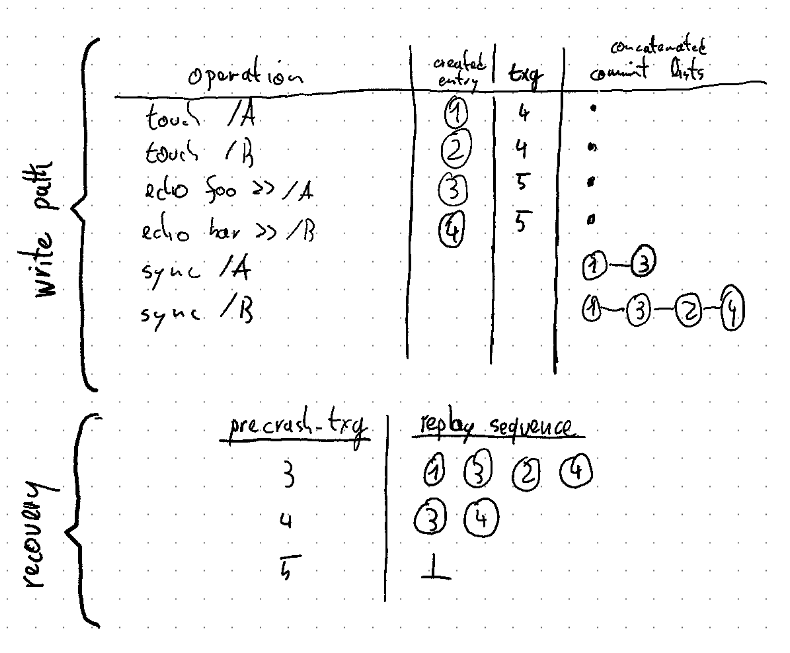
\includegraphics[trim=0cm 0.42cm 0cm 0.42cm]{fig/zil_writepath_and_replay_sequence_logical_level.pdf}
    \caption{
        Example log structure resulting from a series of VFS operations, and the corresponding replay callback invocations for different values of $precrash\_txg$.
        Note that \lstinline{fsync /A} not only logs \lstinline{create /A} and \lstinline{write to /A} but also \lstinline{create /B} since file creation is always placed on the itxg's \textit{sync list}.
        Second, note how records 1 and 2 are skipped during replay if $precrash\_txg = 4$.
        If they were not skipped, the replay callback would fail to create file /A when replaying record 1 because /A already exists in the on-disk state of txg 4.
    }
    \label{fig:zil_writepath_and_replay_sequence_logical_level}
\end{figure}

Note that replay only re-enacts the logical changes to the dataset but does not necessarily restore the exact physical state of the dataset that would have been synced in the absence of a crash.
For example, changes that would have been spread across transaction groups 23, 24, and 25 at write time may land in transaction groups 42 and 43 during replay.
Further, the system could crash again during replay.
For example, a power outage could cause txg 42 to be the last-synced txg whereas 43 was still in \textit{syncing} state.
Since the replay callbacks for the individual log records are \underline{\smash{not idempotent}}, the ZIL must ensure that, after a crash during replay, the changes that were already replayed in transaction group 42 are not replayed again.
For example, the second replay attempt could apply the remaining set of changes in transaction group 83.
(But it may also happen that they are spread over several txgs, e.g., 83 and 84).
The consequence for any ZIL implementation is that it needs to persist the following data:
\begin{description}[noitemsep,leftmargin=1.5cm,labelindent=1cm]
    \item[Precrash-txg] The \textit{precrash-txg} for open logs at the first time during pool import so that it can filter log records by that criterion, and
    \item[Replay progress] Information that tracks which log records have already been replayed so that replay can be resumed at the correct log record after a crash.
\end{description}

\subsection{ZIL(-LWB) Persistence}\label{ch:openzfs_background:zillwb_persistence}

The upstream ZIL implementation uses a singly-linked list of so-called \textit{log-write blocks} (LWBs) to represent the on-disk log structure.
The block pointer to the first LWB is stored in the \textit{ZIL header} structure of the filesystem's or ZVOL's object set.
Each LWB contains a contiguous sequence of the variable-length log records.
The basic structure is depicted in Figure~\ref{fig:zil_lwb__physical_structure_overview}.

\begin{figure}[H]
    \centering
    % make it fit on this page...
    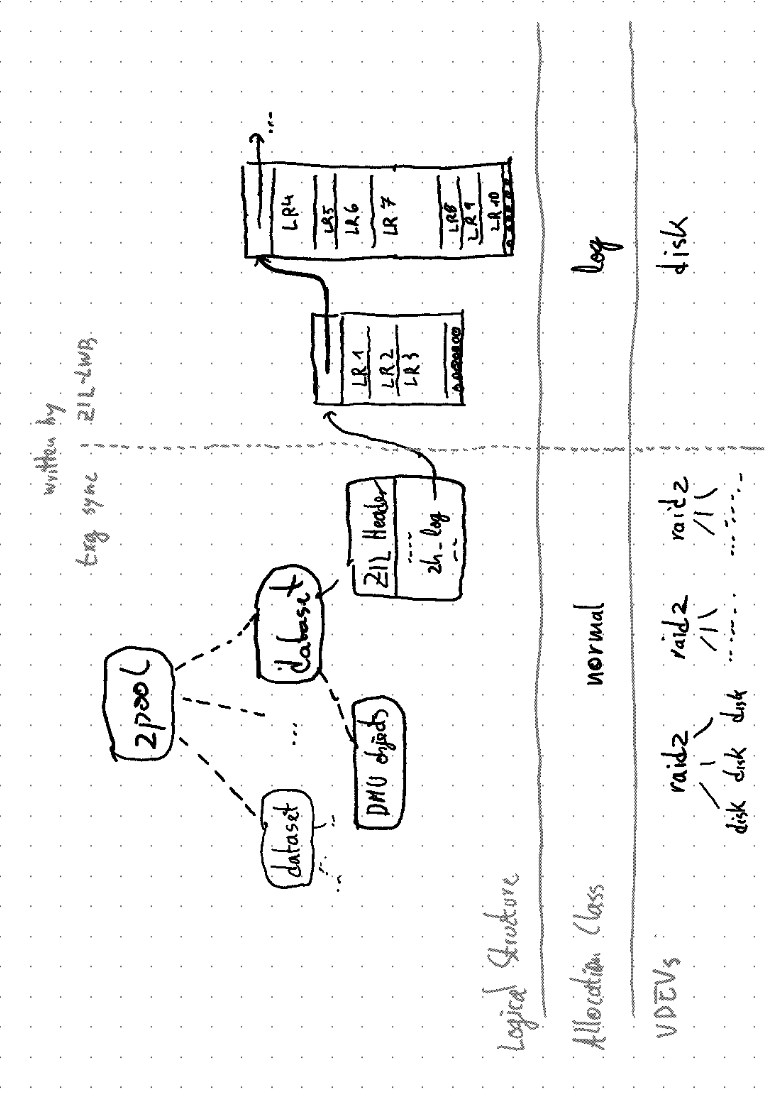
\includegraphics[trim=0cm 0.3cm 0cm 0.3cm, clip]{fig/zil_lwb__physical_structure_overview}
    \caption{On-disk structure of ZIL-LWB as described in the previous paragraph.}
    \label{fig:zil_lwb__physical_structure_overview}
\end{figure}

After \lstinline{zil_commit} has produced the commit list, it iterates over it and appends the log record representation of each ITX to an in-DRAM buffer that will become the new tail LWB in the chain.
Once this buffer is full, it is issued to disk in the background and the procedure continues with a new tail LWB.
The packing of $N$ log records on the commit list into $M$ fewer but larger LWBs has been advantageous in the past:
\begin{description}[noitemsep]
    \item[Latency Amortization]
        Under the assumption that disk latency ($lat_{disk}$) dominates overall synchronous IO latency, writing log records one-by-one would result in a total latency of $N * lat_{disk}$.
        In contrast, grouping records into $M << N$ LWBs reduces the latency to $M * lat_{disk}$
    \item[LWB Timeout / Group Commit]
        ZIL-LWB uses a \textit{timeout} mechanism to extend the amortizing effect of LWB packing.
        As explained above, when a thread $A$ packs log records into LWBs $L_1 \dots L_n$, it issues the IO operations for all but the last LWB $L_n$.
        A releases its lock on the LWB chain and goes to sleep, waiting for another thread $B$ to continue to fill $L_n$.
        If such a thread $B$ \lstinline{zil_commit}s to the same dataset within that time window, it might fill $L_n$ completely and issue it to disk, making $L_{n+1}$ the new tail LWB.
        The IO completion callback for $L_n$ then wakes up $A$ and which is now allowed to return from \lstinline{zil_commit} because the last entry on its commit list is now fully persisted.
        If no thread other threads picks up $L_n$, a timeout wakes up $A$ so that it can issue the IO operation itself.

        Without this mechanism, thread $B$ would need to wait for the last LWB of $A$ to be persisted, \textit{and} for its own LWBs to be persisted because $B$'s first LWB is pointed to by $A$'s last LWB.
        By sharing the last LWB of $A$ and $B$, up to $1 * lat_{disk}$ of waiting time can be avoided.
        Note that whereas ZFS refers to this mechanism as \textit{LWB timeout}, the technique is well-established in disk-oriented databases under the name \textit{group commit} or \textit{commit group}.

    \item[Space Efficiency]
        Log records are stored as a contiguous sequence within the LWB.
        This avoids fragmentation if the commit list consists of small log records because many such log records can be packed into the smallest LWB (4~KiB).
        However, the on-disk format does not allow for splitting of individual log records.
        If the log record cannot be split in software (\lstinline{WR_NEED_COPY}), the open LWB is issued with wasted space and a new LWB is allocated for the log record.
        Conversely, if the current LWB is large but only a few small entries need to be committed, a mostly empty LWB will be issued.
\end{description}

LWBs present a special case for ZFS's on-disk format because the LWB chain is \textit{rooted} in the tree structure that is written by txg sync but \textit{extended} independently by the ZIL.
The solution is to pre-allocate LWBs such that the first LWB's block pointer is stored in the ZIL so that the first LWB of the chain can be found during recovery.
The first LWB's content and any subsequent LWBs in the chain are written and allocated by the ZIL.
However, this represents a special case for the on-disk structure because, unlike all blocks written by \textit{txg sync}, an LWB's content and checksum is not known at the time that the block pointer is written to the ZIL header or the ancestor LWB in the chain.
Thus, instead of storing the checksum in the block pointer, it is stored in the LWB itself --- LWBs are \textit{self-checksumming}.
The full procedure for appending an LWB to the chain thus consists of the following steps:
\begin{enumerate}[noitemsep]
    \item Wait until the LWB is filled or the timeout triggers the LWB to be issued.
    \item Predict the best size for the next LWB based on a simple heuristic.
    \item Allocate the next LWB from the SPA, preferably from a SLOG (next section).
    \item Store the resulting block pointer in the current LWB so that it points to the next LWB.
    \item Compute the checksum of the current LWB.
    \item Repurpose the current LWB's block pointer field to store the computed checksum.
    \item Write out the current LWB.
\end{enumerate}
The checksum ensures crash-consistency of the append operation since a partially written block is assumed to have an invalid checksum.
And even in the case where no crash occurs, ZIL-LWB relies on an invalid checksum to detect the end of the LWB chain during recovery.
(It is assumed unlikely for an unwritten but allocated LWB to be mistaken for an already written LWB because of additional metadata repeated in each LWB that must match for all LWBs in a chain.)
For OpenZFS native encryption, the LWBs are not checksummed but encrypted and authenticated using an AEAD algorithm such as \lstinline{aes-256-gcm}.

LWB that only contain obsolete entries (their maximum txg $\le$ last synced txg) are garbage-collected by \textit{txg sync}.
Every time \textit{txg sync} visits the object set to construct the new version of the on-disk structure, it unlinks LWBs from the head of the chain whose maximum txg is $\le syncing\_txg$ until it reaches an LWB that contains at least one log record for a txg $> syncing\_txg$.
The unlinking updates the chain's head block pointer in the ZIL header but, due to the atomic nature of txg sync, the update only becomes visible on disk if $syncing\_txg$ successfully finishes syncing.
In that case, $syncing\_txg$ becomes the new $precrash\_txg$ txg and thus all entries in the freed LWBs are by definition obsolete.

We visualize both the append and garbage-collection operations in Figure~\ref{fig:zil_lwb__physical_structure_append}.

\begin{figure}[H]
    \centering
    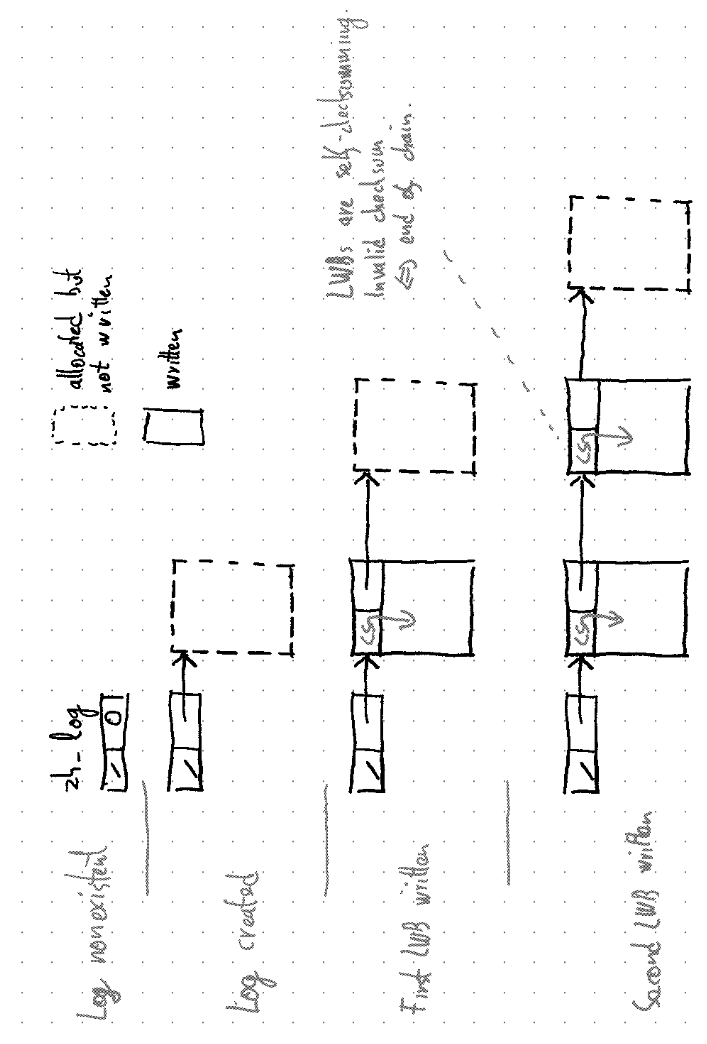
\includegraphics{fig/zil_lwb__physical_structure_append}
    \caption{Visualization of how the LWB chain is extended by the ZIL and garbage-collected by \textit{txg sync}.
    }
    \label{fig:zil_lwb__physical_structure_append}
\end{figure}

\subsection{Separate Log Devices (SLOGs) \& Allocation Classes}

By default, the SPA uses the same VDEVs for \textit{txg sync}'s tree blocks and the ZIL's LWB allocations.
However, it is possible to mark some of the pool's VDEVs as \textit{separate log devices} (SLOGs).
If a SLOG is present, the SPA uses it exclusively and preferentially for LWB allocations.
As hinted in Figure~\ref{fig:zil_lwb__physical_structure_overview}, a typical configuration is the use high-capacity HDDs in a space-efficient \textit{raidz} configuration for the main pool and a costlier but faster NVMe drive (\textit{disk} VDEV) as a SLOG.
Thereby, the advantages of both storage media are combined.
Note that SLOGs only need very limited capacity (tens of GiBs at most) since any LWB is guaranteed to be obsolete after three txgs.

SLOGs were the earliest cross-media capability added to ZFS.
They have recently evolved into a more general feature called \textit{allocation classes}~\cite{openzfsAllocationClasses}.
When VDEVs are added to a zpool, they are assigned to an allocation class.%
\footnote{
 Actually, allocation classes are implemented at the level of \textit{metaslab groups}, which are coarse chunks of VDEV space.
 However, from the user's perspective, allocation group assignment happens at the VDEV level.
}
Functions that allocate space from the SPA must also specify the desired allocation class.
If an allocation succeeds, the space is guaranteed to be located on a VDEV within the specified class.
The following classes exist in upstream ZFS:
\begin{description}[noitemsep,leftmargin=1.5cm,labelindent=1cm]
    \item[aux] A second-level victim cache for ZFS's primary in-DRAM cache or for hot spare devices.
    \item[special] A recently added class for small allocations (still $\ge$ block size).
    \item[dedup] Deduplication table data.
    \item[log] The allocation class used for LWBs.
    \item[normal] The default allocation class. Often used as a fallback if the preferred class has no available space.
\end{description}
Allocation classes are relevant for this thesis because we introduce a new allocation class called \textit{exempt} in Section~\ref{sec:zilpmemzilkind:spacereservation}.

\subsubsection{ZIO Pipeline}
% We briefly mentioned in an earlier section that all reads and writes to SPA-allocated space (DVAs) must go through the SPA to enforce decoupling of the DMU and the storage hardware.

The unified infrastructure for all IO performed by ZFS is the \textit{ZIO pipeline}.
As suggested by its name, ZIO implements a pipeline execution model to execute IO operations.
To issue IO operations, consumers of ZIO allocate a \lstinline{zio_t} object and annotate it with the pipeline stages that it needs to pass through.
Among others, there are pipeline stages that abstract DVA allocation, DVA resolution, checksum computation, compression, block-level deduplication, encryption, and VDEV IO.
The pipeline execution is heavily parallelized using \lstinline{taskq} which are comparable to the Linux kernel's work queues or a dynamically scaling thread pool in userspace.

The ZIO pipeline is relevant for the ZIL because it uses ZIO to write its LWBs.
Integrating LWB IO into the ZIO pipeline is also beneficial for the case where the pool does not have a SLOG configured because the latency-sensitive LWB operations can be prioritized over \textit{txg sync} which is purely throughput-oriented.
However, as we will show in the next chapter, ZIO comes with significant latency overhead, which results in sub-par performance of ZFS on low-latency storage devices such as PMEM.

\chapter{ZIL-LWB on PMEM}\label{ch:lwb_analysis}
Our motivation for this thesis is the significant overhead of the current ZIL implementation (ZIL-LWB) in 4k random synchronous write workloads compared to the performance of the raw PMEM hardware in the same workload.
In this chapter, we describe how we measured this overhead (Section~\ref{ch:lwb_analysis:setup}) and present the resulting data (Section~\ref{ch:lwb_analysis:results}).
In Section~\ref{ch:lwb_analysis}, we proceed with an analysis of the distribution of wall clock time among the different ZFS components under this workload.
Our findings, presented in Section~\ref{ch:lwb_analysis:breakdown}, show that approximately 80\% of the overall latency is spent on persisting LWBs, most of which is software overhead.
We conclude that ZIL-LWB's structure and the ZIO pipeline as its persistence mechanism are unfit to take advantage of PMEM-level performance, motivating the development of ZIL-PMEM.

\section{Benchmark Setup}\label{ch:lwb_analysis:setup}
Our main evaluation system has the following hardware configuration:
\begin{description}[noitemsep,leftmargin=1.5cm,labelindent=1cm]
    \item[CPU] 2 x Intel(R) Xeon(R) Silver 4215 CPU \@ 2.50GHz
    \item[Mainboard] Supermicro X11DPi-N(T)/X11DPi-NT, BIOS 3.1a 10/16/2019
    \item[DRAM] 16 x Micron 8GiB DDR4 2933MT/s (18ASF2G72PDZ-2G9E1), evenly distributed across sockets.
    \item[NVMe] 3 x Micron PRO 960GB NVMe, 512 byte namespace format (MTFDHBA960TDF)
    \item[PMEM] 4 x Intel Optane DC Persistent Memory, 128 GB, (NMA1XXD128GPS), two per socket.
\end{description}
We use the following software stack:
\begin{description}[noitemsep,leftmargin=1.5cm,labelindent=1cm]
    \item[Kernel] Linux 5.9, Debian buster (5.9.0-0.bpo.5-amd64)
    \item[Userland] Debian GNU/Linux (buster)
    \item[fio] fio-3.23-28-g7064
    \item[bpftrace] bpftrace v0.12.0
    \item[bcc] v0.16.0-11-ga74413b0
    \item[OpenZFS] Our tree of OpenZFS with support for \textit{ZIL kinds} (Section~\ref{ch:zilkinds}).
        For this experiment, we use the ZIL-LWB ZIL kind.
        Note that using our tree rather than upstream OpenZFS is (slightly) favorable to ZIL-LWB because our tree contains performance optimizations in the ITX code that are shared among all ZIL kinds.
\end{description}
We use the following system configuration:
\begin{itemize}[noitemsep]
    \item We leave SMT enabled, resulting in 16 hardware threads per socket.
    \item To rule out NUMA effects, we disable the entire second CPU in software using the \lstinline{isolcpus=8-15,24-31} kernel command line parameter.
    \item We configure all Optane DIMMs in \textit{AppDirectNotInterleaved} mode.
    \item We create a 40~GiB-sized \textit{fsdax} namespace on the region of the first DIMM on the first socket.
    \item We create a 40~GiB-sized \textit{devdax} namespace on the region of the first DIMM on the first socket.
    \item We partition each of the 3 NVMe drives into 10 equal-sized partitions each.
    \item We create a zpool called \texttt{dut} with the 30 partitions as top-level VDEVs, and the \textit{fsdax} namespace's /dev/pmem device as a SLOG.
        The reason for the large number of partitions is that we observed slightly improved txg sync performance, presumably due to a higher degree of parallelism towards the NVMe drives.
    \item We create 8 datasets in the zpool, named \lstinline{dut/ds$i}, mounted at \lstinline{/dut/ds$i}.
    \item For all datasets, we configure \lstinline{recordsize=4k} to match the fio workload and set \lstinline{compression=off} to avoid CPU overhead in the ZIO pipeline during txg sync.
\end{itemize}

We use \textit{fio}\todo{ref} to generate a workload of random 4KiB writes (\lstinline{blocksize=4k} and \lstinline{rw=randwrite}).
Each of 1--8 \lstinline{numjobs} threads performs random synchronous write system calls to a separate file per thread (\lstinline{ioengine=sync}, \lstinline{sync=1}, \lstinline{direct=0}, \lstinline{fsync=0}).
Each file has a size of \lstinline{size=100MiB} which means that the written data volume grows with \lstinline{numjobs}, but the amount of dirty data (max.~800~MiB) remains well below the NVMe drive's bandwidth limits.
To avoid scalability-bottlenecks in the ITX code, we place each thread's file onto a separate dataset using the option \lstinline{filename_format=/dut/ds$jobnum/fio_file}.
For each \lstinline{numjobs} value, we measure for one minute (\lstinline{time_based=1}, \lstinline{runtime=60}), with a ramp-up time of 2~seconds (\lstinline{ramp_time=2}), and set \lstinline{end_fsync=1}.
Before we run the benchmark, we prepare the job files using the \lstinline{create_only=1}.

We run this fio workload on the following storage configurations:
\begin{description}[noitemsep,leftmargin=1.5cm,labelindent=1cm]
    \item[zil-lwb] The zpool with ZIL-LWB ZIL kind as described above.
    \item[async] The same configuration as above, but with \lstinline{sync=disabled} set on all datasets.
        This setting effectively disables the ZIL (thereby violating the synchronous semantics) and serves as an upper bound for the performance that can be achieved by any ZIL implementation.
        The remaining work done by \textit{async} is only CPU- and/or DRAM-bound, i.e.,  DMU object modification and ITX allocation (ref. Figure~\ref{fig:zil_api_syscall_activity_diagrams}).
    \item[fsdax] The fio configuration above, applied directly to the /dev/pmem0 block device (\lstinline{direct=1} instead of \lstinline{direct=0}, and \lstinline{filename=/dev/pmem0} instead of \lstinline{filename_format=...}).
        This configuration demonstrates the performance of the Linux block device emulation around the PMEM hardware. It includes the syscall overhead.
    \item[devdax] The fio configuration above, with \lstinline{ioengine=dev-dax}, applied directly to the \texttt{/dev/dax} namespace (\lstinline{filename=/dev/dax0.1} instead of the \lstinline{filename_format} option).
        In this configuration, fio mmaps the PMEM namespace directly and thereby bypasses the kernel completely.
\end{description}

% \begin{description}
%     \item[ioengine] sync
%     \item[end_fsync] 1
%     \item[size] 100MiB
%     \item[blocksize] 4k
%     \item[rw] randwrite
%     \item[time\_based] 1
%     \item[runtime] 60 seconds
%     \item[ramp\_time] 2 seconds
%     \item[sync] 1
%     \item[direct] 0
%     \item[fsync] 0
%     \item[numjobs] We vary this variable from 1 to 8.
%     \item[group_reporting] 1
% \end{description}

\section{Results}\label{ch:lwb_analysis:results}

The following graphs show the achieved IOPS and per-thread latency by \lstinline{numjobs}.

\begin{figure}[H]
    \centering
    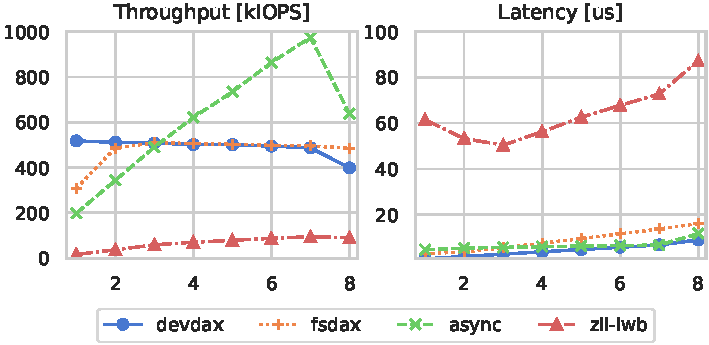
\includegraphics{fig/evaluation/fio4k__lwb_iops_and_lat.pdf}
    \caption{IOPS and latency ZIL-LWB compared to ZFS in async mode as well as the raw fsdax and devdax device.}
    \label{fig:lwbanalysis:iops_and_latency}
\end{figure}

ZIL-LWB only achieves approximately 10k IOPS at one thread and peaks at approximately 100k IOPS at seven threads.
In contrast, ZFS in \textit{async} mode starts with 200k IOPS with one thread and achieves over 900k IOPS at seven threads.
This exceeds the performance of the PMEM hardware which mostly stays at 500k IOPS and demonstrates that the ZIL is clearly the bottleneck in the \textit{zil-lwb} configuration.
A look at the per-IOP average latency emphasizes the vast overhead that ZIL-LWB adds compared to what is possible with the raw PMEM hardware.
Whereas ZFS in async mode only requires 5~us per IOP with \lstinline{numjobs=1}, and raw writes to fsdax require approximately 3~us, ZIL-LWB with the same PMEM hardware as SLOG takes more than 60~us per write.
The minimum latency achieved by ZIL-LWB is at \lstinline{numjobs=4} at approximately 50~us before it starts increasing to up to 85~us at \lstinline{numjobs=8}.
Note that we do not use the results from the \textit{dev-dax} as a baseline for PMEM hardware because the IOPS and latencies reported by fio do not match.
For example, fio reports less than 1~us of latency but only reports 550k IOPS for \textit{dev-dax} at \lstinline{numjobs=1} whereas $\frac{1}{1~us/IOP} = 10^6~\si{IOPS}$ would be anticipated at this latency and thread count.
Figure~\ref{fig:lwbanalysis:zoomed_latency} shows the same latency data as Figure~\ref{fig:lwbanalysis:iops_and_latency} above, albeit zoomed to a scale that allows us to distinguish \textit{dev-dax}, \textit{fsdax}, and \textit{async} latencies.

\begin{figure}[H]
    \centering
    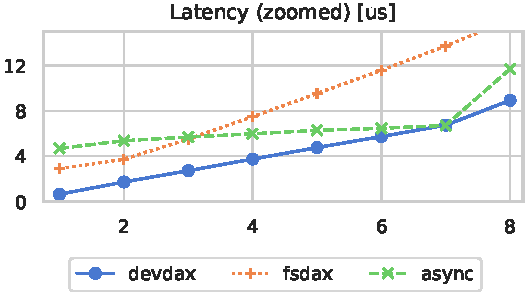
\includegraphics{fig/evaluation/fio4k__lwb_lat_zoomed.pdf}
    \caption{Zoomed section of the latency plot in Figure~\ref{fig:lwbanalysis:iops_and_latency}.}
    \label{fig:lwbanalysis:zoomed_latency}
\end{figure}

\section{Analysis}\label{ch:lwb_analysis:breakdown}

By comparing the numbers for \textit{async} and \textit{zil-lwb}, it is safe to assume that regardless of the value for \lstinline{numjobs}, ZIL-LWB adds at least 40~us of latency.
We want to determine where this time is spent.

We use dynamic instrumentation (eBPF via bpftrace\todo{ref}) to sum up the wall clock time spent in ZFS functions that are executed by the fio threads during a synchronous write operation.
We then use the model in Figure~\ref{fig:lwbanalysis:breakdown_model} to compute the time spent in the asynchronous part of the write operation, the ITX layer, and ZIL-LWB specific code.
We visualize the results as stacked bar charts in Figure~\ref{fig:lwbanalysis:breakdown_charts}.

\begin{figure}[H]
    \centering
    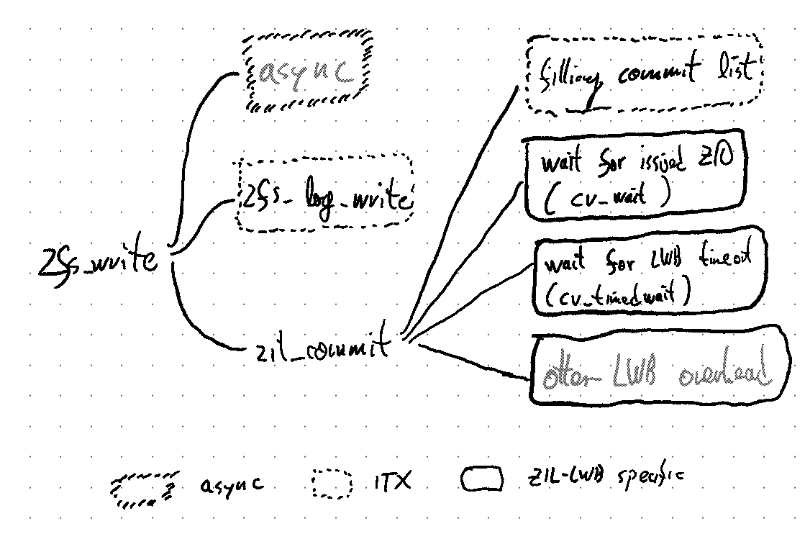
\includegraphics{fig/zil_lwb_latency_analysis__breakdown}
    \caption{Our model of the time spent in ZFS by a fio thread that performs a write system call.
    The different columns represent the different levels of the dynamic call graph.
    The nodes in each column describe all activity that happens at this level of the call graph.
    The wall clock time spent in activities with a solid border style is measured using eBPF instrumentation.
    A dashed border style indicates that the value was computed in post-processing by subtracting the sum of the column's instrumented activities from the parent's value in the column to the left.
    For example, to compute \textit{async}, we compute \lstinline{zfs_write_vnode_op - (zil_commit + zfs_log_write)}.
    The color indicates the subsystem to which we attribute the respective activity.
    }
    \label{fig:lwbanalysis:breakdown_model}
\end{figure}

\begin{figure}[H]
    \centering
    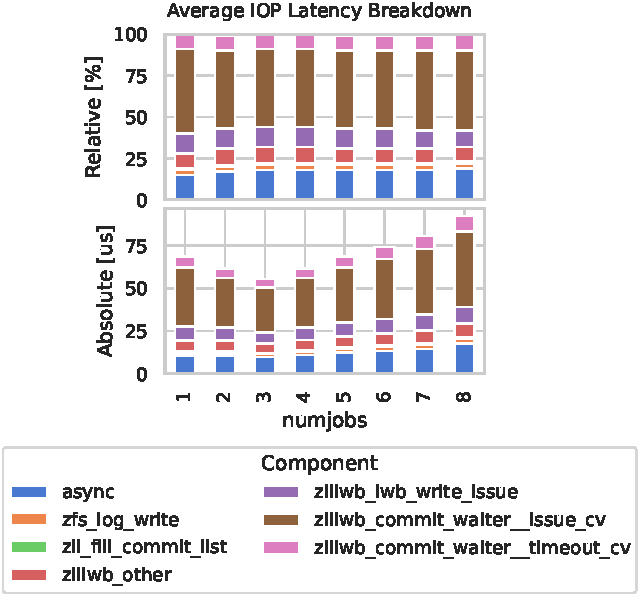
\includegraphics{fig/evaluation/zillwb_latency_analysis.pdf}
    \caption{The relative and absolute breakdown of latency by activity.
    The absolute breakdown is normalized by the number of write operations.
    We compared the latencies in the breakdown with the latencies observed by fio to ensure that our accounting is correct under the given model.
    }
    \label{fig:lwbanalysis:breakdown_charts}
\end{figure}

Our observations are as follows:
\begin{itemize}[noitemsep]
    \item The instrumentation overhead is 5--10~us per IOP. (We compared the latencies that fio reports for the instrumented and uninstrumented run.)
    \item The relative distribution of latency remains mostly unchanged for the different values of \lstinline{numjobs}.
    \item The \textit{async} part of the write path and the ITX layer together only amount to approximately 20\% of overall latency.
        The remaining 80\% are spent on LWB-specific activities.
    \item The LWB timeout mechanism amounts to 4\% of overall latency.
    \item At least 20\% of overall latency are spent on filling LWBs, issuing their corresponding ZIOs, and other LWB-related activities.
    \item 45--50\% of overall latency is spent waiting for the ZIO pipeline to persist the LWBs.
        In absolute numbers, the value ranges from 25--40~us.
        We have separately confirmed that ZIL-LWB uses 12~KiB LWBs which is the smallest possible LWB size allowed by the implementation.
        In our benchmarking setup (per-thread datasets), each LWB only holds a single 4~KiB write log record with 192~B of additional metadata.
        This amounts to write amplification of 3x.
        However, even with this increased data volume per IOP, the results from the previous experiment suggest that with a conservative estimate of 3~us per 4k write to the raw PMEM hardware, we should expect less than 9~us of PMEM write time per LWB.
        Thus, a major fraction of the 25--40~us that are spent waiting for ZIO is actually pure software overhead.
\end{itemize}

Our observations lead us to the following conclusions:

\textbf{First, we have reason to believe that the high overhead of ZIO is unlikely to be reduced} to a degree that allows for exploitation of PMEM-level latency, regardless of whether the hardware is actual PMEM or simply very fast NVMe drives.
The reason is that there is an inherent conflict of goals for ZIO:
whereas the ZIL is strictly latency-oriented, all other consumers (\textit{txg sync}, \textit{scrubbing}, \textit{zfs send/recv}) are throughput-oriented.
The pipeline-oriented, parallelized architecture of ZIO is important for throughput and provides great flexibility, but increases latency through context switches.
This problem is well known in the ZFS community, see \cite{openzfsZILPerformanceImprovements2020,ZFSSubredditRichardYaoCommentsOnPoorSynchronousWritePerformance,OpenZFSGithubIssueNVMeReadPerformanceZioPipeliningOverheadTimChaseComment}.

\textbf{Second, the persistent representation of the ZIL as a chain of LWBs poses a severe and unnecessary overhead on PMEM.}
For one, the latency amortization provided by LWBs and the timeout mechanism is unnecessary at PMEM-level latencies where it is cheaper to persist the log records on an individual basis than batching them in LWBs and coordinating with other threads on the matter.
And for another, since PMEM is byte-addressable, the persistent representation is no longer constrained by disk block sizes, opening up the possibility of better space efficiency.

\chapter{Design Overview}\label{ch:designoverview}
Given the insights described in the previous chapter, we propose an alternative ZIL implementation called \textbf{ZIL-PMEM} that exclusively targets PMEM SLOG devices.
In this chapter we define the project goals for ZIL-PMEM and provide a high-level overview of its design.
The subsequent two chapters then introduce the core data structure and our approach to integrating it into ZFS.

\section{Project Goals \& Scope}

\newcommand{\csgoal}[1]{\textbf{#1}}

\subsection{Requirements}\label{sec:requirements}

\csgoal{Coexistence}
ZIL-PMEM must coexist with ZIL-LWB in code and at runtime due to limited availability of PMEM hardware and the limitations of the ZIL-PMEM design.

\csgoal{Same Guarantees}
ZIL-PMEM must maintain the same crash consistency guarantees towards user-space as ZIL-LWB for both ZPL and ZVOL.

\csgoal{Simple Administration \& Pooled Storage}
Pooling of storage resources and simple administration are central to ZFS~\cite{bonwickZettabyteFileSystem2003}.
ZFS should automatically detect that a SLOG device is PMEM and, if so, use ZIL-PMEM for all of the pool’s datasets.
No further administrative action should be required to fully benefit from ZIL-PMEM.

\csgoal{Correctness}
In the absence of PMEM media errors and data corruption, ZIL-PMEM must be able to replay all data that it reported as committed.
The result must be the same as if ZIL-LWB had been used in lieu.
Specifically:
\begin{itemize}[noitemsep,beginpenalty=100000,midpenalty=100000]
    \item Replay must respect the logical dependencies between log records.
    \item Logging must be crash-consistent, i.e., the in-PMEM state must always be such that replay is correct.
    \item Replay must be crash-consistent, i.e., if the system crashes or loses power during replay, it must be possible to resume replay after the crash.
        Resumed replay must continue to respect logical dependencies of log records.
\end{itemize}

\csgoal{Data Integrity}
Data integrity is a core feature of ZFS~\cite{bonwickZettabyteFileSystem2003}.
ZIL-PMEM must detect corrupted log records using an error-detecting code.
Detected corruption must be handled \textit{correctly} (as outlined in the previous paragraph) and \textit{gracefully} with the following behavior as the baseline:
``Assume a sequence of log records $1 \dots N$ where log record $1$ does not depend on a log record and each record $i > 1$ depends on its predecessor $i-1$.
Data corruption in record $i \in 1 \dots N$ must not prevent replay of records $1 \dots i-1$".

\csgoal{Low Latency}
The latency overhead of ZIL-PMEM compared to raw PMEM device latency for the same data volume should be minimal for single-threaded workloads.
Multi-threaded workloads are addressed below.

\csgoal{Multi-Core Scalability}
Since PMEM is added as a pool-wide resource used by all of the pool's datasets, ZIL-PMEM should scale well to multiple cores.
Barring PMEM throughput limitations, the speedup in throughput (IOPS) achieved by parallelizing synchronous IO to multiple cores on a ZIL-PMEM system should be as follows:
{
\setlength{\parskip}{0pt}
\begin{description}[topsep=0pt, noitemsep, leftmargin=1cm, labelindent=1cm, widest=1 private dataset per thread]
    \item[1 private dataset per thread] Always near-linear speedup.
    \item[1 shared dataset] \mbox{}
          \begin{description}[noitemsep, leftmargin=1cm, labelindent=1cm, widest=ZPL filesystem]
              \item[ZPL filesystem] No speedup.
              \item[ZVOL] No speedup in standard mode, potentially sub-linear speedup in bypass mode (Section~\ref{sec:itxgbypass}).
          \end{description}
\end{description}
}

\csgoal{Maximum Performance On Intel Optane DC Persistent Memory}
We develop and evaluate ZIL-PMEM exclusively for/on Intel Optane DC Persistent Memory since it is the only broadly available non-volatile main memory product on the market.
Whereas supercapacitor-backed persistent memory modules (NVDIMM-N) should be usable with ZIL-PMEM, our goal is to design a system that makes optimal use of the Optane hardware.

\csgoal{CPU-Efficient Handling Of PMEM Bandwidth Limits}
If the maximum write bandwidth to any kind of storage device is exceeded, the IO stack must somehow apply back-pressure to avoid losing in-flight data.
With PMEM, the IO stack is the CPU microarchitecture and the back-pressure manifests as stalling instructions.
However, from the OS thread scheduler's perspective, threads whose instructions stall because they wait for PMEM are indistinguishable from actually busy threads.
\citeauthor{yangEmpiricalGuideBehavior2020} have shown that a single Optane DIMM's write bandwidth can be exhausted by one CPU core at 2~GB/s and that write bandwidth decreases to 1~GB/s at ten or more CPU cores.
% In contrast, DRAM shows a near-linear increase in bandwidth to 60~GB/s at 15~threads.~\cite[fig.4]{yangEmpiricalGuideBehavior2020}
Since ZIL-PMEM shares PMEM among all datasets in a zpool, we expect bandwidth exhaustion to be a phenomenon that wil happen in practice.
ZIL-PMEM should thus provide a mechanism to shift excessive PMEM IO wait time off the CPU.

\csgoal{Testability}
ZIL-PMEM must be architected for testability.
The core algorithms must be covered by unit tests.
Further, ZIL-PMEM should be integrated into the ztest user-space stress test as well as the SLOG tests of the ZFS Test Suite.

\subsection{Out Of Scope For The Thesis}
The following features were omitted to constrain the scope of the thesis.
We believe that our design can accommodate them without major changes.

\csgoal{Support For OpenZFS Native Encryption}
The ZIL-PMEM design presented in this section does not address OpenZFS native encryption.
Intel Optane DC Persistent Memory supports transparent hardware encryption per DIMM at zero overhead\todo{cite spec}.
In contrast, OpenZFS native encryption is per dataset and software-based.
Given these significant differences in data and threat model, ZIL-PMEM cannot rely on Optane hardware encryption.
Instead, ZIL-PMEM would need to invoke OpenZFS native encryption and decryption routines when writing or replaying log entries.

\csgoal{Protection Against Scribbles}
Scribbles are software bugs that cause accidental overwrites of PMEM, e.g., due to incorrect address calculation or out-of-bounds access in any piece of kernel code.
PMEM-specific filesystems such as PMFS and NOVA-Fortis have already introduced mechanisms to protect against scribbles~\cite{dulloorSystemSoftwarePersistent2014,xuNOVAFortisFaulttolerantNonvolatile2017}.
We believe that these mechanisms can be applied to our design as well.

\subsection{Limitations}
The following features are deliberately not addressed by our design.
More experimentation and experience with ZIL-PMEM will be necessary to determine which features are useful in practice, how they can be realized, and how they interact with the existing requirements.

\csgoal{No NUMA Awareness}
\citeauthor{yangEmpiricalGuideBehavior2020} recommend to ``avoid mixed or multi-threaded accesses to remote NUMA nodes. [...]  For writes, remote Optane’s latency is 2.53x (ntstore) and 1.68x higher compared to local"~\cite{yangEmpiricalGuideBehavior2020}.
We do not account for this behavior in the design and do not evaluate ZIL-PMEM in a NUMA configuration.\todo{future work}

\csgoal{No Data Redundancy}
ZIL-PMEM provides data integrity protections but does not provide a mechanism for data redundancy.\todo{future work}

\csgoal{Only Works With SLOGs}
Our approach to integrate ZIL-PMEM into ZFS is only applicable to PMEM SLOGs and does not work for a zpool that uses PMEM as main pool VDEVs.
Such pools continue to use ZIL-LWB.

\csgoal{No Software Striping}
Our design only supports a single PMEM SLOG device.
Users may wish to use multiple PMEM DIMMs to increase log write bandwidth.
With Intel Optane DC Persistent Memory, multiple PMEM DIMMs can be interleaved in hardware with near-linear speedup~\cite{yangEmpiricalGuideBehavior2020}.
Whereas software striping would be the natural approach to ZFS, it will be non-trivial to achieve the same speedup as hardware-based interleaving.

\csgoal{No Support For \lstinline{WR_INDIRECT}}
ZIL-LWB writes the data portion of large write log records directly to the main pool devices.
The ZIL record then only contains metadata such as \lstinline{mtime} and a block pointer to the location in the main pool.
This technique avoids double-writes which is particularly advantageous if the pool does not have a SLOG, which in turn is a use case that ZIL-PMEM does not address (see above).
Further, if a SLOG is available, \lstinline{WR_INDIRECT} log record write latency is likely to be dominated by the main pool's IO latency if it consists of regular block devices.
If the main pool's IO latency were acceptable, a fast NVMe-based ZIL-LWB SLOG or no SLOG at all would likely be sufficient for the setup in question.

\csgoal{Space Efficiency}
ZIL-PMEM is allowed to trade PMEM space for time and simplicity when presented with the option.
Our justification is twofold.
First, PMEM capacities are significantly higher than DRAM.
For example, the smallest Intel Optane DC Persistent Memory DIMM offered by Intel is 128~GiB.
Second, the maximum amount of log entry space required from any ZIL implementation is a function of the maximum amount of dirty data allowed in the zpool.\todo{ref background section? this sentence should remain, though}
For ZIL-LWB, small SLOG devices of \SI{16} to 32~GiB are sufficient in practice \cite{OpenZFSDocsWorkloadTuningSynchronousIO}.
Thus, there is sufficient headroom for PMEM space usage in ZIL-PMEM.

\section{Design Overview}\label{sec:designoverview}
We add the concept of \textit{ZIL kinds} to ZFS.
A zpool's ZIL kind is a pool-scoped variable that determines its strategy for persisting the ZIL to stable storage.
The ZIL's record format, logical structure, and code that creates and replays log records remains shared among all ZIL kinds.
The default ZIL kind is \textit{ZIL-LWB}, but if a zpool has exactly one SLOG and that SLOG is Persistent Memory, its ZIL kind is \textit{ZIL-PMEM}.
ZIL-LWB uses the SPA to allocate log-write blocks (LWBs) from the storage pool with a bias towards SLOG devices (ref. Section~\ref{ch:openzfs_background:zillwb_persistence}).
For ZIL-PMEM, we exempt the PMEM SLOG's allocatable space from block allocation to use directly for \textit{PRB/HDL}, our PMEM-specific data structure.

We partition the PMEM space into fixed-size contiguous segments called \textit{chunks}.
We develop a data structure called PRB that consumes these chunks and exposes the abstraction of an unordered persistent storage layer for \textit{log entries}.
A log entry is the unit of data that can be written to and read from PRB.
It consists of the ZIL's log record and PRB-specific metadata.
PRB scales to many concurrent writers and features a mechanism to avoid excessive on-CPU waiting for PMEM~IO.
Log entries that are stored in PRB are automatically garbage-collected when they become obsolete after their transaction group has been synced out.

PRB provides a pool-wide storage substrate for log entries but does not define any structure.
This is the role of the \textit{HDL} abstraction which implements a mostly sequential log structure on top of PRB.
Each dataset in the zpool has a separate HDL to which it writes log entries.
The HDL adds metadata to its entries to enable reconstruction of the log's logical structure.
After a system crash, each HDL scans PRB for entries that need to be \textit{replayed} for recovery of the respective dataset's committed state.
Replay happens in a deterministic sequential order and is crash-consistent.
Loss of entries, e.g., due to data corruption, is handled as gracefully as possible under the constraints of the logical dependencies encoded in the log structure.

The role of the ZIL-PMEM ZIL kind is to integrate PRB/HDL into ZFS by
hooking into the SPA to construct the PRB,
synchronizing HDL and dataset lifecycles, and
adapting between the ZIL and the HDL domain.
Figure~\ref{fig:zilpmem_architecture} visualizes the resulting system architecture.

The next two chapters describe our design in detail.
Chapter~\ref{ch:prbhdl} describes our main contribution --- the PRB/HDL data structure.
The integration of PRB/HDL into ZFS is then presented in Chapter~\ref{ch:zilpmem}.

\begin{figure}[H]
    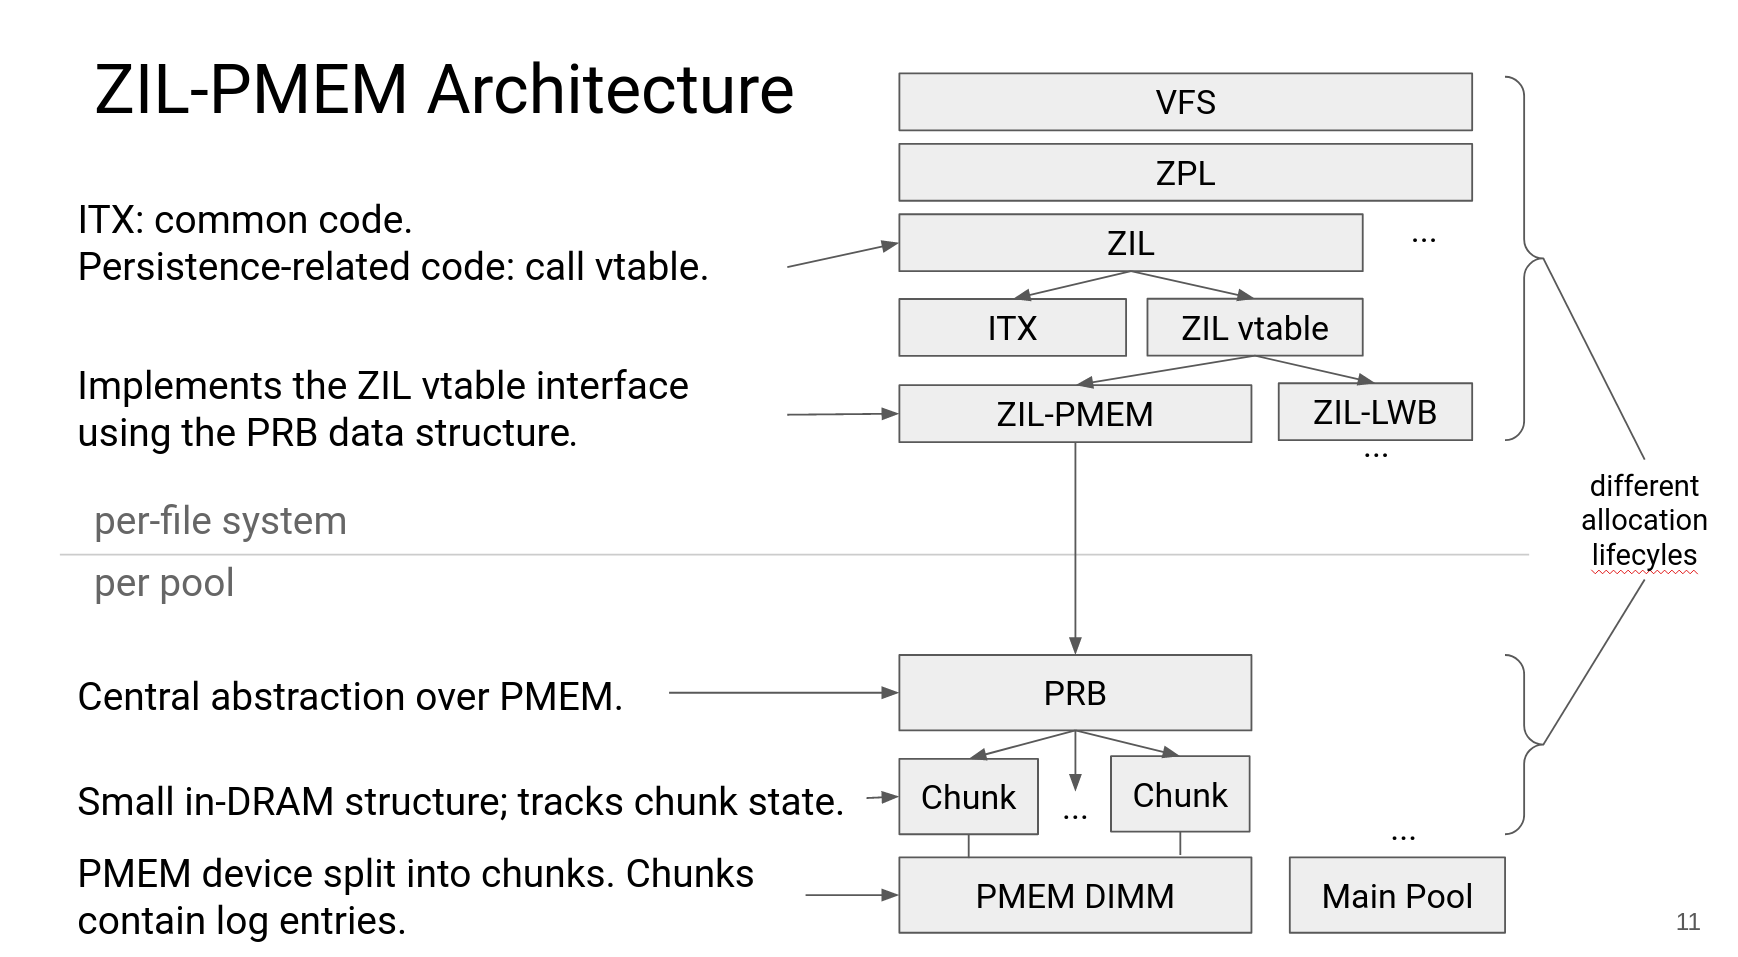
\includegraphics{fig/zilpmem_architecture_overview}
    \caption{Overview of the system architecture as described in this section.}
    \label{fig:zilpmem_architecture}
\end{figure}

\chapter{The PRB/HDL Data Structure}\label{ch:prbhdl}

In this chapter we describe the PRB/HDL data structure.
PRB consumes chunks of PMEM and provides a scalable storage substrate for an arbitrary number of HDLs which in turn provide the abstraction of a persistent, garbage collected log.
In Chapter~\ref{ch:zilpmem}, we then present how we integrate PRB/HDL into ZFS as the ZIL-PMEM ZIL kind.

We present the design and implementation of PRB in a top-down manner.
In Section~\ref{di:prb:analysis} we isolate the requirements that ZIL-PMEM puts on PRB by recapitulating how the ZIL fits into ZFS's overall architecture.
Afterwards, in Section~\ref{di:prb:approach}, we give a high-level overview of our design.
Section~\ref{di:prb:logstructure} presents the virtual log abstraction that is exposed by HDL and Section \ref{di:prb:replayapproach} describes the high-level approach for replay.
Sections \ref{di:prb:deptrack}, \ref{di:prb:modeldatacorruption}, and \ref{di:prb:ccrecovery} then progressively refine our understanding of replay and explain how data corruption and crash-consistency is addressed by HDL.
Subsequently, we describe PRB which is the storage substrate that the HDLs use for persistence:
Sections~\ref{di:prb:dramdatastructure} and \ref{di:prb:pmemdatastructure} present the data structures that we use for PMEM space management and log entry storage.
In Section~\ref{di:prb:traversal} we describe the algorithm that traverses the in-PMEM data structure during log recovery.
Section~\ref{di:prb:gc} explains how garbage collection removes obsolete from PRB.
The low-latency and CPU efficient design of the write path is then presented in Section~\ref{di:prb:write}.
Finally, Section~\ref{di:prb:api} provides a walkthrough of the API that is consumed by ZIL-PMEM.

\section{Context \& Requirements}\label{di:prb:analysis}

Remember from Section~\ref{sec:openzfs_background} that all ZPL filesystem state is represented as DMU objects.
When a filesystem call modifies DMU objects, it must do so from within a DMU transaction $T_i$ that belongs to a transaction group $T_{i_{txg}}$.
After the system call handler has completed the DMU transaction by calling \lstinline{dmu_tx_commit(T_i)}, the logical change $C_i$ made in $T_i$ is not yet persisted to stable storage.
Instead, the DMU accumulates the changes from many DMU transactions in DRAM as so-called \textit{dirty state}, grouped by the transaction's transaction group (txg).
This dirty state is eventually persisted to ZFS's on disk state in a procedure that, through copy-on-write techniques, is atomic at the granularity of txgs (\textit{txg sync}).

The ZIL bridges the gap between txg syncs so that synchronous VFS operations can return to userspace, even though their DMU transaction's txg has not yet been synced to disk.
For that purpose, each VFS operation summarizes each logical change $C_i$ that it makes per DMU transaction $T_i$ as an \textit{intent log transaction}~(ITX).
Before completing the DMU transaction through \lstinline{dmu_tx_commit}, it \textit{assigns} the ITX to the ZIL.
Synchronous VFS operations call \lstinline{zil_commit} before returning to userspace to append the ITXs that are relevant to the operation to a sequential persistent log.

In upstream OpenZFS, the only available implementation of this persistent log is the chain of \textit{log write blocks} (LWBs) which we described in Section~\ref{ch:openzfs_background:zillwb_persistence}.
With the introduction of ZIL kinds (details in \ref{ch:zilkinds}), the persistence layer becomes pluggable:
whereas the shared \textit{itxg} data structure continues to determine the \textit{commit list} that describes which ITXs need to be persisted in what order, the ZIL kind is free to represent the log structure however it sees fit.

Regardless of the persistence strategy, all ZIL kinds must implement the same interface to recover committed state (\lstinline{zil_replay}).
The ZPL invokes \lstinline{zil_replay} during the mounting procedure of a filesystem.
It provides a callback that the ZIL kind must invoke for precisely those log records (= encoded ITXs) whose changes $C_i$ were lost in the crash.
(Their txg $T_{i_{txg}} > precrash\_txg$ where $precrash\_txg$ is the last synced transaction group before the system crashed.)
The callback re-applies the change encoded in the log record, thereby recovering the committed state.

The reader should remember that the set and order of log records for which the callback is invoked is not necessarily intuitive because
a) ITXs may be reordered by the ITXG structure and b) the log records must be filtered by $precrash\_txg$.
We refer to Figure~\ref{fig:zil_writepath_and_replay_sequence_logical_level} in Section~\ref{openzfs:the_zil_api} to an example and more details.


We derive the following abstract view of \textbf{what} needs to be stored \textbf{per log}:
\begin{itemize}[noitemsep,beginpenalty=100000,midpenalty=100000]
    \item The log records themselves.
    \item The transaction group of the DMU transaction that the log record encodes.
    \item Structural information that defines replay order and/or logical dependencies between log records that replay must respect.
    \item For replay, the precrash txg to discern replayable from obsolete log records (see previous section).
    \item For replay, some representation of \textit{replay progress} to enable resumption of replay if the system crashes during replay.
        (The log record format and replay callbacks are not idempotent.)
\end{itemize}

For ZIL-PMEM, we put the following requirements on the PRB/HDL:
\begin{itemize}[noitemsep,beginpenalty=100000,midpenalty=100000]
    \item On the write path, the overhead added to the raw log record write time should be minimal.
    \item It must scale well on a multicore system since many datasets write their log records in parallel.
        This scalability requirement includes efficient use of CPU time in case the PMEM write bandwidth is exceeded.
    \item It must garbage-collect log records after they are obsoleted by \textit{txg sync} and/or finished replay.
    \item It must provide the replay interface described above.
    \item It must detect data corruption using checksums. (Repair and redundancy are out of scope for this thesis, see Section~\ref{sec:requirements}.)
\end{itemize}

\section{Approach}\label{di:prb:approach}
We introduce the pool-wide \textit{PRB} object which abstracts a set of contiguous segments of PMEM (\textit{chunks}) as a persistent, unordered set of \textit{log entries}.
A log entry is a ZIL log record and associated metadata.
More abstractly, a log entry encodes a logical change to a dataset that was applied in a single DMU transaction.
PRB provides facilities for adding log entries to the set and for iterating over its contents.
It automatically garbage-collects entries after they become obsolete after their transaction group has been synced out.

Log entries are not written directly to PRB but instead to the \textit{HDL} object of the dataset that they affect.
A HDL is a virtual log built on top of PRB that organizes the entries for a single dataset in a mostly sequential structure.
After a system crash, the HDL provides a replay facility that recovers the replayable entries, orders them according to their logical dependencies, and handles missing entries.

At any time, there exists one HDL for each head dataset in the pool.
They are set up early during pool import and torn down late during export.
If a dataset is created or destroyed, the corresponding HDL is set up or torn down as well.
HDL is stateful.
Its internal states represent the different phases that a dataset goes through with regard to the ZIL.

\begin{figure}[H]
    \centering
    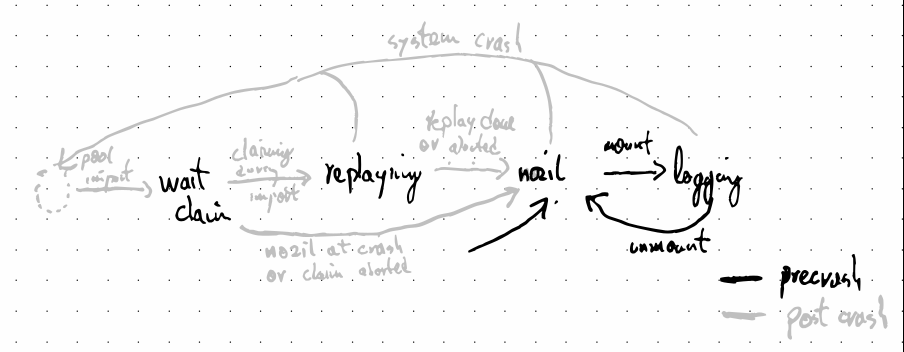
\includegraphics[height=5cm]{fig/prb_hdl_runtime_states}
    \caption{The runtime states of a HDL.}
\end{figure}

When the HDL is created, it does not have a log and is in state \textit{nozil}.
When the dataset is mounted, the HDL allocates a \textit{log GUID} and persists it to the ZIL header.
The log GUID uniquely identifies the log's entries in the PRB.
The HDL is now in state \textit{logging} and threads can write entries to it.
If the dataset is unmounted, the log GUID is discarded and the log transitions back to state \textit{nozil}.
Otherwise, the HDL remains in state \textit{logging} until the system crashes.

When a zpool is imported, the import procedure examines the ZIL header of each dataset to recover the HDL's runtime state from before the crash.
If the HDL state was \textit{nozil}, there is nothing to do and the HDL transitions to that state.
If the HDL state was \textit{logging} or \textit{replaying}, it must be claimed before txg sync starts.
For HDLs in state \textit{logging}, the claiming procedure saves the zpool's \textit{last synced} txg as the \textit{precrash-txg} and transitions the HDL and ZIL header to state \textit{replaying} in the initial replay position.
If the HDL was already in state \textit{replaying} at import time, the precrash-txg and replay position are recovered from the ZIL header.
At this point, all HDLs are either in state \textit{nozil} or \textit{replaying} but claiming is not yet complete.
For every HDL in state \textit{replaying}, the claiming procedure scans the PRB for log entries that need to be held back for replay.
Entries that are held back by at least one HDL are exempt from PRB's garbage collection.
After this scanning step is complete, the claiming phase is over and the txg sync thread starts.
HDLs are not replayed until their dataset is mounted by the user. %which can be deferred indefinitely by the user, might not happen for several zpool import/export cycles, or system crashes.
After replay is complete, the HDL discards the log GUID and transitions to state \textit{nozil}.
At this point, the mount procedure behaves as if log replay had not happened and starts a new log with a new log GUID, thereby closing the circle.
Note that the HDL (and PRB) are able to recovery from system crashes in all states.
We describe how we handle this issue in Section~\ref{di:prb:ccrecovery}.

\section{HDL: Log Structure}\label{di:prb:logstructure}
The structure of the virtual log that each HDL represents is defined by metadata stored with each entry that is written to PRB.

We \textbf{attribute} entries to a given HDL's log through the \textit{log GUID}:
\begin{description}[noitemsep,leftmargin=1.5cm,labelindent=1cm]
    \item[Log GUID] A 128 bit random identifier stored in the HDL's ZIL header and repeated in every entry written through that HDL.
\end{description}

The following pieces of metadata define the structure of the log.
\begin{description}[noitemsep,leftmargin=1.5cm,labelindent=1cm]
    \item[Transaction Group (txg)] The transaction group in which the change encoded in the entry was or would have been synced out by txg sync.
    \item[Generation Number (gen)] The log is a sequence of generations, each of which contains many log entries.
        The generations encode logical dependencies between entries.
        Entries within the same generation do not depend on each other.
        Entries from newer generations unconditionally depend on all entries in all previous generations.
        We represent generations as unsigned 64-bit non-zero integers.
    \item[Generation-Scoped ID (gsid)] Within a generation, we identify entries by another by the $gsid$, another unique unsigned 64-bit non-zero integer.
        As the name suggests, the $gsid$ only needs to be unique within a generation.
\end{description}
Note that the tuple $(gen, gsid)$ uniquely identifies an entry within a log.

We visualize the structure of the log in a grid.
The rows represent the transaction group ($txg$) and the columns represent the generation ($gen$).
For readability, we represent entries not by $(gen, gsid)$ but by a single unique letter.
The projection of entries onto the horizontal axis shows the dependency relationship encoded by the generations.
The projection of entries onto the vertical axis shows the sets in which entries are garbage-collected.

\begin{figure}[H]
    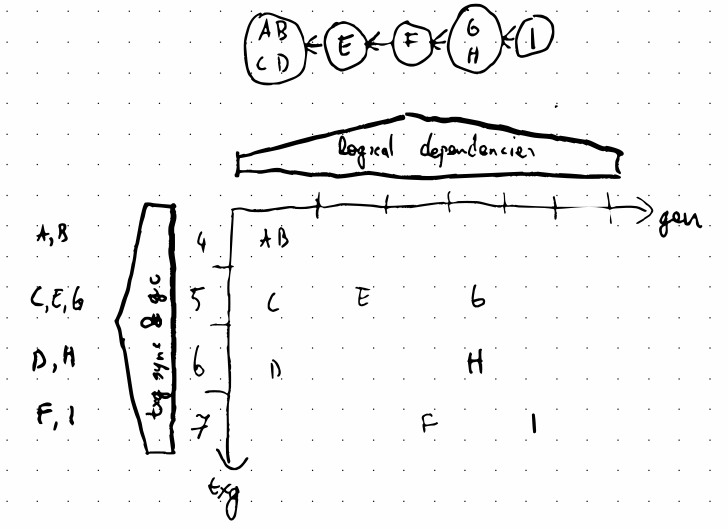
\includegraphics{fig/prb_hdl_log_structure_example}
    \caption{Structure of a single HDL's log as described in the previous paragraph.}
    \label{fig:prb_hdl_log_structure_example}
\end{figure}

\section{HDL Replay: Basic Approach}\label{di:prb:replayapproach}
Replay must apply the changes that were successfully logged to the HDL but whose DMU transaction did not sync before the system crashed.
To accomplish this task, it scans the PRB for entries that belong to the HDL and determines a \textit{replay sequence} $S$.
\begin{align*}
    & \text{Entry}~E_i \in S \\
    \Leftrightarrow & E_i.log\_guid = HDL.log\_guid \wedge E_i.txg > precrash\_txg
\end{align*}
$S$ is sorted in \textit{replay order}, which is the order in which the changes encoded in the entries need to be applied.
Given two entries $E_a$, $E_b \in S$ for the same HDL, the replay order is a total order defined by
\begin{align*}
    & E_a <_{replay} E_b \\
    \Leftrightarrow &  (E_a.gen, E_a.gsid) <_{lexicographical} (E_b.gen, E_b.gsid) \\
    \Leftrightarrow & E_a.gen < E_b.gen \vee (E_a.gen = E_b.gen \wedge E_a.gsid < E_b.gsid) \\
\end{align*}
For our example in Figure~\ref{fig:prb_hdl_log_structure_example}, this results in the following replay sequences, depending on the value of $precrash\_txg$.


\begin{figure}[H]
    % https://www.tablesgenerator.com/#
    % fig_src/static/prb_hdl_log_structure_example__replay.tgn
    \centering
        \begin{tabular}{r|l|l|l|l|l|l|l|l|l|}
        \multicolumn{1}{l|}{}              & \multicolumn{9}{c|}{Replay Sequence} \\
        \multicolumn{1}{c|}{precrash\_txg} & A  & B  & C  & D & E & F & G & H & I \\ \hline
        3                                  & x  & x  & x  & x & x & x & x & x & x \\
        4                                  &    &    & x  & x & x & x & x & x & x \\
        5                                  &    &    &    & x &   & x &   & x & x \\
        6                                  &    &    &    &   &   & x &   &   & x \\
        7                                  &    &    &    &   &   &   &   &   &   \\ \cline{2-10} 
    \end{tabular}
    \caption{Replay sequences for the log depicted in Figure~\ref{fig:prb_hdl_log_structure_example}, by $precrash\_txg$. }
    \label{fig:prb_hdl_log_structure_example__replay}
\end{figure}

We use a total order so that we can precisely encode replay progress by storing the last-replayed $(E.gen, E.gsid)$.
This is necessary for crash consistency because log entry replay is not idempotent.
We revisit this topic in Section~\ref{di:prb:ccrecovery}.

Note that the definition of the replay order does not account for overflows of $gen$ or $gsid$ --- entries written after the overflow would be incorrectly ordered as ``$<_{replay}$'' entries written before the overflow.
Overflows could be handled in software, e.g., by temporarily destroying the log of the dataset and creating a new one with a fresh log GUID.
However, our implementation has no such provisions because even with the (absurdly) conservative value of 1~ns write time per log entry, the first overflow event would only occur in 584~years if $gen$ starts at~$1$.

\section{HDL Replay: Dependency Tracking}\label{di:prb:deptrack}
% \begin{description}
    %     % \item[Garbage Collection] After a txg $t_{synced}$ has been synced, PRB garbage-collects all entries $\mathcal{E}_{gc} := { E : E.txg \le t_{synced}}$.
    %     %     This does not interfere with replay because, if the system crashes, it is guaranteed that $precrash\_txg \le t_{synced}$ and hence $\mathcal{e}_{gc}$ would never be part of a replay sequence.
    %     \item[Loss of Entries] If such a missing entry $E_m$ with $E_m.txg > precrash\_txg$ is missing, any entry $E_d$ that logically depends on $E_m$ ($E_m < E_d$) and is for an unsynced txg ($E_d.txg > precrash\_txg$) must no longer be replayed.
        % However, all entries $E_p$ that do not depend on $E_m$ ($E_p \le E_m$) and need replay ($E_p.txg > precrash\_txg$) should still be replayed.
    % \end{description}
Replay is complicated by the fact that the entries that were stored in the PRB can be lost.
For example, bitflips in PMEM might corrupt the entry's log GUID or PRB-internal metadata.
If an entry $E_m$ with $E_m.txg > precrash\_txg$ is missing, any entry $E_d$ that logically depends on $E_m$ ($E_m < E_d$) must no longer be replayed.
However, all entries $E_p$ that do not depend on $E_m$ and need replay should still be replayed (their $E_p \le E_m \wedge E_p.txg > precrash\_txg$).

We detect missing entries through a set of counters that we store in the metadata of each entry.
For an entry $E$, the counter $E.C_{ctxg_i}$
\begin{gather*}
    E.C_{ctxg_i} := \#\{ D : D.gen < E.gen \wedge D.txg = ctxg_i\}
\end{gather*}
stores the number of entries that were written to the log since its inception, for a DMU transaction with txg $ctxg_i$, until generation $E.gen$.
During replay, we first construct the replay sequence (example in the previous section, Figure~\ref{fig:prb_hdl_log_structure_example__replay}).
Then, we re-compute and compare the counters for each entry in the replay sequence.
If an entry $E_m$ has been lost, the counters of any dependent entry $E_d$ (their $E_d.gen > E_m.gen$) will not match, causing replay to stop with $E_d$ as a \textit{witness}.
Missing entries in the last generation (the ``tail'' of the log) cannot be detected with this scheme.

The per-txg scoping of the counters is critical to accommodate garbage collection.
Suppose we only used a single sequence counter for all log entries of a HDL.
After a txg $t_{synced}$ has been synced, PRB garbage-collects all entries $\mathcal{S}_{gc}$ that are obsolete:
\begin{align*}
    \mathcal{S}_{gc} := \{ E : E.txg \le t_{synced}\}
\end{align*}
These entries no longer show up when the claiming or replay procedures scan the PRB for entries with the HDL's log GUID.
If we used a single sequence counter to check for missing entries, we would be unable to discern garbage-collected entries from missing entries.

It is sufficient to include only those counters $E.C_{txg_i}$ in the entry metadata whose transaction groups $txg_i$ had not yet been synced at the time that $E.gen$ started.
The reason is that a) the replay sequence only contains entries in unsynced txgs and b) $E$ only depends on entries $D$ with $D.gen < E.gen$.
Since there are only three possible unsynced txgs at any time (\textit{open}, \textit{quiescing}, \textit{syncing}), we only need to store three $(txg_i, C_{txg_i})$ tuples per log entry.
In fact, since txgs never skip a number, we only store the value of $txg_{open}$ and recompute
\begin{align*}
    txg_{quiescing} & = txg_{open} - 1 \\
    txg_{sycing} & = txg_{open} - 2
\end{align*}
\todo{compact encoding is just an idea, not in impl yet}

We use the same algorithm to compute the counters on both the write and recovery path.
This works because the write path must use monotonically increasing generation numbers, and the entries in the replay sequence are sorted in that order.
The counters are stored in a table called \textit{live table}.
It has four rows $R_i := (txg, ctr), i \in \{0,1,2,3\}$.
When an entry $E$ is written or visited, it modifies the counter in the row with index $I_T := T \bmod 4$ where $T := E.txg$.
We distinguish the following conditions:
\begin{itemize}[noitemsep]
\item If $R_{I_T}.txg = T$, we simply increment $R_{I_T}.ctr$ and are done.
\item If $T > R_{I_T}.txg$, we can infer that txg $R_{I_T}.txg$ must have been synced out because there are only three unsynced txgs at any given time but four array entries that are reused circularly, courtesy of indexing by $T \bmod 4$.
In that case, we can discard the state in the row and reuse it for $T$ by setting $R_{I_T} \leftarrow (T, 1)$.
\item Conversely, if $T < R_{I_T}.txg$, we can infer that the entry we are writing is for an already synced txg and hence obsolete.
In that case, we do not change the \textit{live table} and turn the entry write operation into a no-op.
Hence, the condition cannot occur during replay. If it does, the write path implementation is incorrect.
\end{itemize}
Note that the use of 4-ary arrays allows the use of \textit{bitwise-and} for indexing, which is a common ZFS idiom (\lstinline{table[txg&3]}).

To detect the start of a new generation, and support resumable replay after a crash (Section~\ref{di:prb:ccrecovery}), we maintain a separate variable $E_{last} := (gen, gsid)$.
When an entry $E$ is written or visited, we compare it to $E_{last}$ using the following rules:
\begin{description}[noitemsep,leftmargin=1.5cm,labelindent=1cm]
\item[$E < E_{last}$] This case is prohibited for writers because the API contract for log writers is that generation numbers must be monotonically increasing.
  During replay, we skip all entries $\le_{replay} E_{last}$ because $E_{last}$ marks the last-replayed entry.
\item[$E.gen = E_{last}.gen$] The writer did not start a new generation and we leave the \textit{last table} unmodified.
\item[$E.gen > E_{last}.gen$] We create a copy of the \textit{live table}. We refer to this snapshot as \textit{last table}.
\end{description}
Regardless of whether a new generation was started or not, we always update $E_{last} \leftarrow E$ and increment the counter in the \textit{live table} as described in the previous paragraph after evaluating the rules above.

The counters $E.C_{txg_i}$ have the same value for all entries in generation $E.gen$  because, by definition, they only count entries written up to but not including $E.gen$.
Hence, we compute them from the \textit{last table} once and cache the results until the next generation is started:
\begin{enumerate}[noitemsep]
    \item Determine row index $i_{max} := \max_{i \in \{0,1,2,3\}} R_i.txg$ where $R_i \in \text{last table}$.
    \item Invariant: $R_{i_{max}}.txg$ is the highest potentially unsynced txg in generations $< open\_gen$.
        We make the most conservative assumption that $R_{i_{max}}.txg$ was the \textit{open txg} in generation $open\_gen - 1$.
    \item Find the counters for \textit{quiescing} and \textit{syncing txg}.
        We scan the \textit{last table} twice to find counters for transaction groups $R_{i_{max}}.txg - 1$ and $R_{i_{max}}.txg - 2$.
        If the \textit{last table} does not contain those counters, we use a value of zero.
\end{enumerate}

Figure~\ref{fig:prb_counters_table__computation_and_encoding} contains an illustration of the process that converts the \textit{last table} into the counters table.
We provide an extensive example in Figure~\ref{fig:prb_counters_table__example}.

\begin{figure}[H]
    \centering
    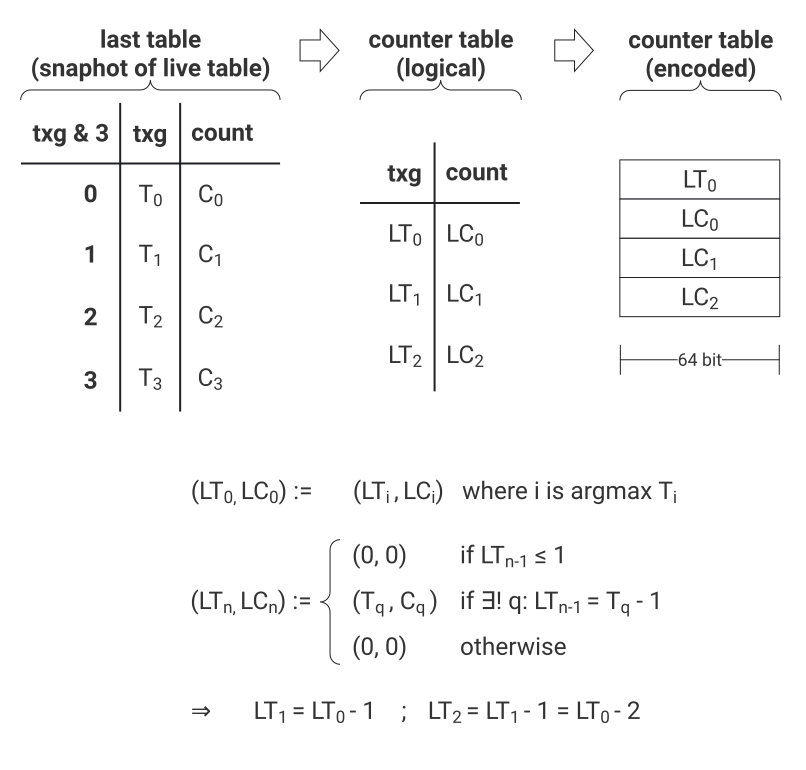
\includegraphics{fig/prb_counters_table__computation_and_encoding}
    \caption{
        Visualization of how the counters table is computed from the \textit{last table} structure.
    }
    \label{fig:prb_counters_table__computation_and_encoding}
\end{figure}

\begin{figure}[H]
    \centering
    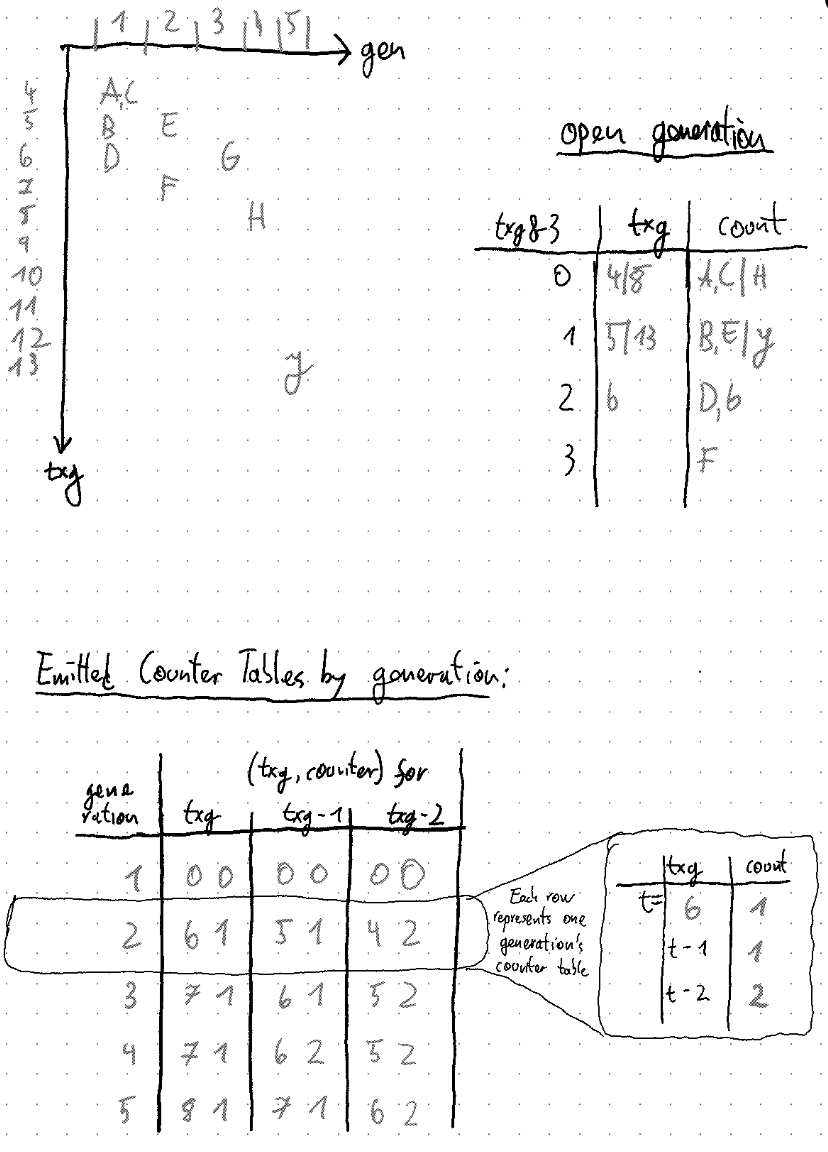
\includegraphics{fig/prb_counters_table__example}
    \caption{
        Example for the computation of the counters that are stored in the entry.
        The following entries are written to the log:
        A,B,C,D in generation 1; E,F in generation 2; G in generation 3; H in generation 4; J in generation 5.
        Note that their txgs differ sometimes but stay in a corridor of at most three txgs.
        The table at the bottom shows the counter values in the entry headers:
        each row represents the counter table that is stored in the entry headers of one generation.
        The table at the upper right shows the \textit{live table}'s content over time.
        Instead of counters, we show the entries that would cause the specific counter to be incremented.
        We visualize row-reuse by separating new row content with a ``\lstinline{|}" symbol in each cell of the reused row.
    }
    \label{fig:prb_counters_table__example}
\end{figure}

\section{HDL: Model For Data Corruption}\label{di:prb:modeldatacorruption}
The use of counters to validate that no log entries are missing during replay relies on the assumption that random data corruption is incapable of ``forging'' new log entries.
If this were possible, a forged entry could compensate a lost entry in the counter table.
The loss of the entry would go unnoticed and the replay of the forged entry would likely corrupt the dataset.

We believe that it is sufficiently unlikely for random data corruption to accidentally forge an entry.
A forged entry would have to fulfill the following requirements to affect counter validation for a given log $L$:
\begin{itemize}[noitemsep]
    \item It must have been correctly added to PRB's data structures such that a scan of PRB will find it during recovery.
        (We address the PRB's data structure in Section~\ref{di:prb:pmemdatastructure}.)
    \item Its \textit{log GUID} value must match log $L$'s log GUID.
    \item Its $(gen, gsid)$ must not collide with the original entries.
        Such a collision would be noticed when constructing the replay sequence.
        (Our implementation uses a b-tree that identifies and sorts nodes by $(gen, gsid)$).
    \item Its \textit{txg} value must be in the correct corridor of unsynced txgs and generation.
        If the txg is too old or too young, the forged entry would be noticed by the dependency tracking code when re-computing the counters.
\end{itemize}

Apart from random data corruption, we have considered the following scenarios and concluded that they are out of scope for ZIL-PMEM:
\begin{itemize}[noitemsep]
\item Implementation errors on the write path.
\item Firmware bugs, e.g., in the Optane DIMM's wear-leveling layers, that could make old entries re-appear.
\item Deliberate injection of log entries by a malicious party with write access to PMEM.
    This needs to be part of the threat model if ZIL-PMEM is extended to support OpenZFS Native Encryption.
    Forged entries should be trivially detectable by cryptographically authenticating the entry header, e.g. using the AEAD ciphers that are already in use for the encryption feature.
\item Accidental reuse of \textit{log GUIDs}.
    If two HDLs use the same log GUID to write their entries, the HDLs will each claim their and the other HDL's entries.
    This scenario is very unlikely because we generate log GUIDs as 128 bit random numbers and check for collisions with other HDLs.
\end{itemize}

\section{HDL: Replay Crash-Consistency}\label{di:prb:ccrecovery}

The PRB and its HDLs must be able to tolerate a system crash at any time in their lifecycle.
With regard to recovery, this means that claiming must be restartable and replay resumable across crashes.
Further, the restarted or resumed recovery procedure must be able to handle online and offline loss of entries due to data corruption.

Crash-consistency for claiming is trivial because it runs during pool import before txg sync starts.
Thus, all changes made by claiming are accumulated in DRAM and atomically persisted by the first transaction group that is synced after pool import.
From the perspective of HDLs that are in state \textit{logging}, this first transaction group is $precrash\_txg + 1$.
If the system crashes before that txg is synced, a subsequent import attempt restarts from the same state as the previous one.
HDLs that are already in state \textit{replaying} make no modifications during claiming --- they only build up DRAM state, i.e., the set of entries held back for replay.

Replay is complicated by two additional aspects:
\begin{itemize}[noitemsep]
    \item Replay of an individual log entry is not idempotent. This is a property of the ZIL log record format and its logical structure and thus a hard constraint.
    \item Replay is spread across several transaction groups and hence not atomic.
        (See this chapter's Section~\ref{openzfs:the_zil_api} on OpenZFS background.)
\end{itemize}
Our solution is to externalize all state of the replay algorithm, including the counters used for dependency tracking, to a structure called \textit{replay state}.
Whenever we replay an entry, we checkpoint \textit{replay state}.
We store the latest checkpoint in the ZIL header every time we replay an entry.
If the system crashes, we recover \textit{replay state} from the checkpoint in the ZIL header.

The following variables are stored in \textit{replay state}:
\begin{description}[noitemsep,leftmargin=1.5cm,labelindent=1cm]
    \item[$\mathbf{(gen_{last}, gsid_{last})}$] The $(E.gen, E.gsid)$ of the last entry $E$ that was replayed. (Corresponds to $E_{last}$ in Secion~\ref{di:prb:deptrack}.)
    \item[Live Table] The \textit{live table} at the time the entry was replayed, i.e., $R_i$ with $i~\in~{0,1,2,3}$.
    \item[Last Table] The \textit{last table} at the time the entry was replayed.
    \item[$E_{seal}$] An artificial entry header that is used to detect lost entries at the end of the log structure.
\end{description}
The crash-safe replay procedure performs the following steps:
\begin{enumerate}[noitemsep,beginpenalty=100000,midpenalty=100000]
    \item \label{ccReplay:claimscan} Claiming reads the log GUID from the ZIL header, then scans the PRB and holds back the log's entries from garbage collection.
    \begin{itemize}[noitemsep,beginpenalty=100000,midpenalty=100000]
        \item \label{ccReplay:transitionToReplaying} If the HDL is in state \textit{logging}, claiming transitions the ZIL header to \textit{replaying} and initializes the \textit{replay state} checkpoint in the ZIL header.
            \begin{itemize}
                \item $(gen_{last}, gsid_{last})$ is $(0, 0)$.
                \item \textit{live table} and \textit{last table} are zeroed out.
                \item $E_{seal}$ is determined as follows.
                \begin{enumerate}
                    \item Construct a temporary replay sequence \\ \mbox{$S_{tmp} = \{E_s : s \in 1, \dots, n\}$}.
                    \item In DRAM, append an artificial entry $E_{n+1}$ to $S_{tmp}$. \\
                        \mbox{$E_{n+1}.gen = E_{n}.gen + 1$}, \mbox{$E_{n+1}.gsid = 1$}, and \\
                        \mbox{$E_{n+1}.txg = E_{n}.txg$}.
                    \item Iterate over $S_{tmp}$ and compute the counter tables.
                        Validate the tables for $E_{1,\dots,n}$.
                        When arriving at $E_{n+1}$, assign the expected table to $E_{seal}$.
                \end{enumerate}
            \end{itemize}
        \item If the HDL is already in state \textit{replaying}, the ZIL header is not modified.
    \end{itemize}
    \item Replay recovers its \textit{replay state} from the checkpoint $C$ in the ZIL header.
    \item \label{ccReplay:construct_sequence} Replay constructs a replay sequence $S$ from the held back entries.
    \item While replaying $S$, the following happens for each entry $E_s \in S$:
        \begin{enumerate}[noitemsep,beginpenalty=100000,midpenalty=100000]
            \item \label{ccReplay:skipreplayed} Skip $E_s$ if it has already been replayed, i.e., \\
            \mbox{$(E_s.gen, E_s.gsid) \le (C.E_{last}.gen, C.E_{last}.gsid)$}. \\
            Otherwise:
            \item Create a backup checkpoint $C_b$ of \textit{replay state}.
            \item Perform dependency tracking as described in the previous section.
            \item Create a checkpoint $C_{E_s}$.
            \item In one DMU transaction, replay $E_s$ and store $C_{E_s}$ in the ZIL header.
            \item If replay fails or the DMU transaction fails, abort the transaction and roll back the in-DRAM version of \textit{replay state} to $C_b$.
    \end{enumerate}
\end{enumerate}

Note that steps~\ref{ccReplay:claimscan}~and~\ref{ccReplay:construct_sequence} construct a \textit{new} replay sequence on every pool import, based on a new scan of PRB.
This allows for handling of offline data corruption in PRB.
Assume that we lose an entry $E_m$ while the system is offline.
If \mbox{$E_m.txg \le precrash\_txg$}, the loss of the entry is unnoticed because $E_m$ is by definition not part of the replay sequence.
If $E_m$ is skipped by step~\ref{ccReplay:skipreplayed}, the loss of the entry might be worth reporting but does not affect replay because it has already been replayed.
Otherwise, dependency tracking will eventually detect that $E_m$ is missing if, and only if, any other entry depends on it.
$E_{seal}$ is an artificial dependency to ensure that lost entries in the last generation are detected.
\todo{this is not yet implemented}

We handle online data corruption as follows.
Claiming and replay only operate on DRAM-buffered copies of the entry metadata called \textit{replay node}.
When replaying an entry, the replay callback is forced to use a special function that attempts to read the entry from PRB and buffers it in DRAM.
Before allowing access to the entry, it ensures that the entry metadata still matches the data in the \textit{replay node}.
If either the read from PRB fails (e.g., due to checksum errors) or if the metadata does not match, we know that the entry has been corrupted since the PRB scan.

Note that the last generation $E_{seal}.gen - 1$ of the log structure is not protected against re-appearing log entries.
Assume that during initial claiming, entries $(42,1)$ and $(42,3)$ in generation $42$ are observed as the last entries of the replay sequence.
Then $(E_{seal}.gen, E_{seal.gsid)}$ is $(43,1)$ and the counter table of $E_{seal}$ only accounts for these two entries, and all previous generation's entries.
Now assume that another entry $(42,2)$ had been written but was temporarily invisible during initial claiming, e.g., due to temporary data corruption.
If for some reason $(42,2)$ becomes visible again, and we start replaying, then $(42,2)$ will be replayed even though it was not visible during claiming.
And if $(42,2)$ were to replace $(42,1)$ or $(42,3)$, we would not even notice the counter mismatch when arriving at $E_{seal}$.
This behavior seems desirable in the sense that replay recovers as much committed data as possible.
However, in combination with WR\_INDIRECT ZIL log records, it can lead to pool corruption.
ZIL-PMEM does not currently support WR\_INDIRECT records due to this problem as well as another WR\_INDIRECT-related issue that also affects ZIL-LWB which we discovered during this thesis~\cite{OpenZFSGithubIssueZilLeaksClaimedBlocksInSeveralEdgeCases}.
Our proposed solution in the \mbox{OpenZFS} issue tracker could be used by ZIL-PMEM to properly detect changes to the last generation after claiming, and to support WR\_INDIRECT if desired.

\section{PRB: DRAM Data Structure}\label{di:prb:dramdatastructure}
After the description of HDL in the previous sections, we now move down to the level of PRB.
The central requirements for PRB are
\begin{itemize}[noitemsep]
    \item persistence of log entries in PMEM,
    \item parallel insertion of log entries from multiple threads and HDLs,
    \item garbage collection of obsolete log entries,
    \item measures to detect data corruption, and
    \item prevention of excessive on-CPU waiting for PMEM IO.
\end{itemize}

Our design is built around the \textit{chunk} abstraction.
A chunk is a contiguous segment of PMEM that acts as an insert-only container for log entries.
PRB's role is to mediate access between HDLs and chunks.
When a thread writes an entry to the conceptual \textit{set of entries} that is the PRB, it actually inserts the entry into one of the PRB's chunks.
Once a chunk is full, PRB lets it sit unmodified until all entries in it are obsolete.
Garbage collection then removes all entries in those obsolete-only chunks and makes them available for reuse by writers.
The PRB scanning done by claiming and replay is implemented as an iteration over the entries in all chunks of the PRB.
If a chunk contains at least one candidate entry for replay, the claiming HDL holds the chunk back from the write path and/or garbage collection.
Note that this design fully decouples storage location (chunk) from log structure (encoded in entry metadata, see previous sections).

Each chunk is represented by a DRAM object that holds the following values:
\begin{description}[noitemsep]
    \item[PMEM location] The chunk's start and end address in PMEM. These values do not change for the lifetime of the chunk.
    \item[Claim refcount] The number of HDLs that claimed at least one entry in the chunk for replay.
        Chunks with non-zero claim refcount are exempt from garbage collection and the write path.
    \item[Max txg] The maximum transaction group of the entries that were written to this chunk.
        This value is used by garbage collection to determine when all entries in the chunk are obsolete.
    \item[Write position] The PMEM address where the next entry will be written.
        We discuss the PMEM layout of the chunk in more detail in Section~\ref{di:prb:pmemdatastructure}.
\end{description}

We move chunks between the following data structures to keep track of their current role within PRB.
\begin{description}[noitemsep]
    \item[Commit Slots]
    PRB maintains a roster of \textit{commit slots}, each of which has an associated \textit{open chunk}.
    When a thread writes an entry through a HDL, the thread first \textit{acquires} a commit slot to gain temporary exclusive access to its \textit{open chunk}.
    Then, it writes the entry to the open chunk and immediately releases the slot so that other threads can acquire it.
    \item[Free List]
    The \textit{free list} holds empty chunks.
    Their \textit{claim refcount} and \textit{max txg} is zero and their write position is reset to the chunk's start address.
    A log writer that needs a new chunk for its commit slot puts the commit slot's current open chunk on the \textit{full list} (see below) and gets a new chunk from the \textit{free list}.
    \item[Full Lists]
    The \textit{full lists} contains chunks that wait for garbage collection.
    PRB maintains one full list for each unsynced txg $T_i$. The \textit{full list} for $T_i$ contains exactly those (full) chunks whose \textit{max txg} is $T_i$.
    After $T_i$ has been synced, garbage collection empties the chunks on $T_i$'s \textit{full list} and moves them to the \textit{free list}.
    Note that it is sufficient to maintain three full lists at any given time --- one for each of the three unsynced transaction groups \textit{open}, \textit{quiescing}, and \textit{syncing}.
    The three lists can be represented as an array of three lists that is indexed by $T_i \bmod 3$.
    The lists are cyclically reused as new transaction groups are born.
    Our implementation follows the common ZFS idiom of using four lists that are indexed by \lstinline{T_i&3} where \lstinline{&} is the \textit{bitwise and} operation.
    \item[Wait Replay List]
    During the claiming phase, all of the PRB's chunks are on the \textit{wait replay list}.
    The HDLs scan the chunks on this list.
    If a chunk contains at least one entry that needs to be held back for replay, the HDL increments the chunk's \textit{claim refcount}.
    Once claiming is done and \textit{txg sync} triggers the first garbage collection cycle, any chunk on this list that has a zero refcount is emptied and moved to the \textit{free list}.
    The list is also scanned for zero refcounts during all future garbage collection cycles to garbage-collect chunks that are no longer held by any HDL because they finished replay.
    Note that it is critical for replay crash consistency to defer garbage collection until \textit{after} the last txg of replay of the last HDL that held the chunk has synced.
    If we garbage-collected entries before the last holding HDL's ZIL header has transitioned to state \textit{nozil} on disk, and crashed in between, the garbage-collected entries might be missing when resuming replay.
\end{description}

Figure~\ref{fig:prb_chunk_ownership_cycle__transitions} visualizes transitions of the chunks over their lifetime.
Figure~\ref{fig:prb_chunk_ownership_cycle__example} provides a corresponding example.

\begin{figure}[H]
    \centering
    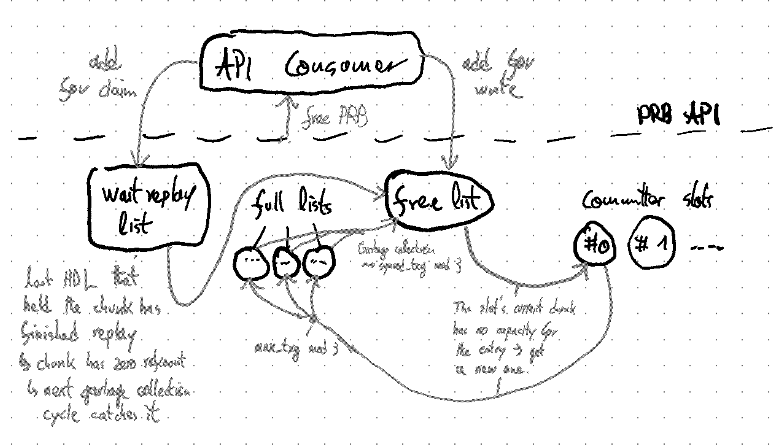
\includegraphics{fig/prb_chunk_ownership_cycle__transitions}
    \caption{The different owners of a chunk and the events that cause transitions of ownership.}
    \label{fig:prb_chunk_ownership_cycle__transitions}
\end{figure}

\begin{figure}[H]
    \centering
    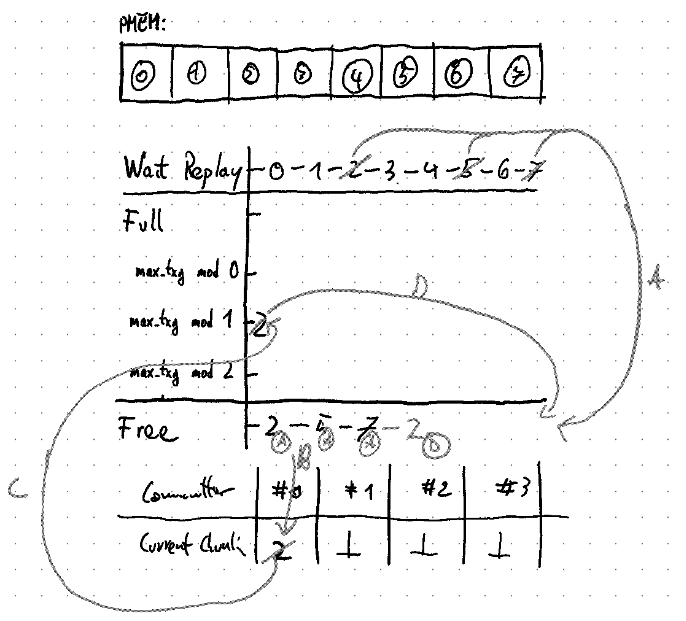
\includegraphics{fig/prb_chunk_ownership_cycle__example}
    \caption{
        Example for transitions of chunk ownership.
        The PRB is constructed with all eight chunks added as \lstinline{_for_claim}.
        Claiming (\textit{A}) determines that chunks 0, 1, 3, 4, and 6 need to remain on the \textit{wait replay list} because they contain entries for HDL logs that need replay.
        Chunks 2, 5, and 7 only contain obsolete entries and move to the \textit{free list}.
        We do not replay any of the logs.
        However, a log writer starts writing a new log in \textit{B}.
        It finds that its commit slot (\#0) has no active chunk.
        Thus, it and moves the first chunk on the \textit{free list} (i.e., chunk 2) to the commit slot.
        After writing the entry to chunk 2 the log writer releases the commit slot.
        Another log writer acquires commit slot \#0 and writes entries to it.
        Chunk 2's capacity is insufficient to hold the last entry (\textit{C}).
        The thread places chunk 2 on the correct \textit{full list} for chunk 2's \textit{max txg} and finds a new chunk on the free list for the commit slot (not shown).
        Eventually \textit{txg sync} triggers garbage collection for the txg that is chunk 2's \textit{max txg} which resets chunk 2's in-PMEM and in-DRAM sequence and subsequently places it back onto the free list.
    }
    \label{fig:prb_chunk_ownership_cycle__example}
\end{figure}

\section{PRB: PMEM Data Structure}\label{di:prb:pmemdatastructure}
As explained in the previous section, PRB is built on top of contiguous segments of PMEM which we call \textit{chunks}.
However, PRB only consumes the chunks, it does not create them.
Chunk allocation is the responsibility of the PRB consumer, i.e., ZIL-PMEM.
This design improves modularity and testability because it decouples the following two concerns:
\begin{description}[noitemsep,leftmargin=1.5cm,labelindent=1cm]
    \item[Resource Acquisition] The PRB consumer is responsible for integrating PMEM SLOG VDEV into the zpool, discovering its memory mapping, and partitioning the PMEM space into chunks.
    \item[PMEM Data Structure] PRB implements the persistent data structure that actually stores entries inside the chunks.
\end{description}
With regard to persistent data structure, this separation of concerns relieves PRB from the need to define structures to track the partitioning of PMEM space into chunks.
It is the consumer's responsibility to provide the PRB with the same set of chunks every time the PRB is constructed.
However, since we do not store absolute addresses, the mapping of each chunk in the virtual address space is allowed to change between PRB constructions.
% Our implementation of ZIL-PMEM uses a simplistic partitioning scheme.
% It uses a hard-coded chunk size of 128~MiB\todo{check} and partitions as an array the allocatable into contiguous segments of that size.
% However, future work 
% \todo{future work: dynamically add and remove chunks}

% When the PRB is constructed, i.e., when the PMEM SLOG VDEV is added to the pool, the consumer initializes the PMEM structure in each chunk before passing them to PRB.
% At all subsequent times when the PRB is constructed, the consumer must pass the same PMEM chunks to PRB's constructor function.
% More precisely, the start addresses of the PMEM chunks are allowed to change but their effective PMEM address range must be the same every time the PRB is constructed.

Entries are variable-length records and are stored within chunks in a contiguous sequence.
Each entry is represented as a fixed-length 256 byte sized header and a variable-length body.
The first entry starts at the chunk's start address which must be aligned to 256 bytes.
The space after each entry is zero-padded to the next multiple of 256 bytes.
The next entry starts after the padding.
The sequence is terminated either explicitly by an invalid entry header or implicitly if the last entry has filled the chunk completely.
Figure~\ref{fig:prb_physical_data_structure__chunklayout} provides an example chunk layout.
Note that the ordering of entries within the chunk has no semantic value as the logical view on the chunk is that of a \textit{set} of entries.

The entry body is a verbatim copy of an opaque byte slice provided by the log writer.
(In ZIL-PMEM, this byte slice is the ZIL log record structure that is shared among all ZIL kinds.)
The entry header's contents are managed by the PRB and HDL.
Its contents are as follows:
\begin{description}[noitemsep,leftmargin=1.5cm,labelindent=1cm]
    \item[HDL-scoped metadata] The metadata required for attribution of a log entry to a HDL and subsequent replay.
    \begin{itemize}
        \item Log GUID
        \item Generation
        \item Generation-Scoped ID
        \item Encoded Counters for dependency tracking.
    \end{itemize}
    \item[Body Length] We store the exact body length in bytes.
    The zero padding in the chunk sequence is not considered part of the entry itself.\todo{fix that?}
    \item[Body Checksum] Fletcher checksum of the body data.
    \item[Header Checksum] Fletcher checksum of the header to ensure data integrity of the metadata.
    If the header checksum is corrupted then none of the other header fields can be trusted.
    \item[Zero Padding] The unused bytes in the header have the defined value of zero.
    Their value is part of the header checksum.
\end{description}

Chunks must be sufficiently large to hold at least one entry because there is no mechanism to split an entry across multiple chunks.
The smallest chunk's size determines the maximum entry size that can be written to PRB.
However, for multicore-scalability, it is advisable to use chunk sizes that are much larger than a single average entry, as we will elaborate on in Section~\ref{di:prb:write}.
%The choice of chunk size is a trade-off between PMEM space-efficiency (fragmentation at the end of the chunk), the acceptable blast radius\todo{this is a common ops term but not sure if academic enough...} of data corruption (traversal, see Section~\ref{di:prb:traversal}), and multi-core scalability on the write path (see Section~\ref{di:prb:write}).

\begin{figure}[H]
    \centering
    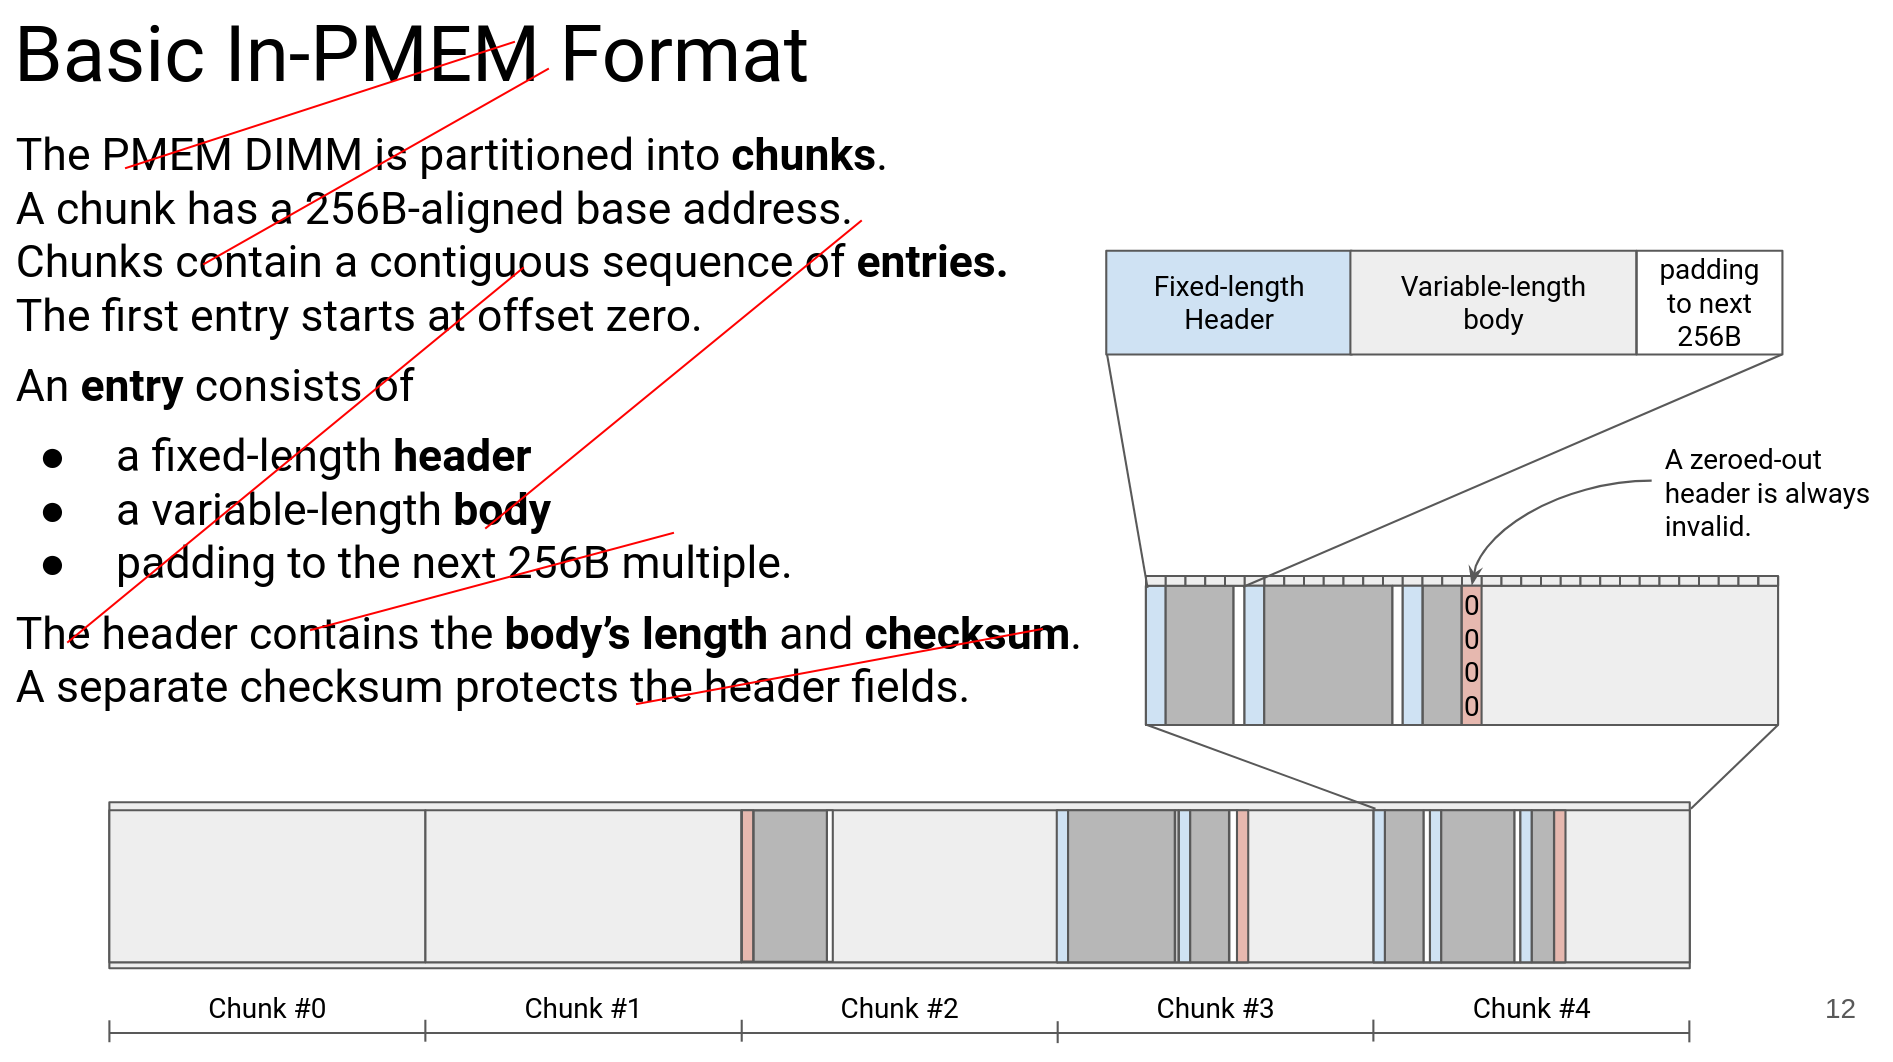
\includegraphics{fig/prb_persistent_structure__chunklayout}
    \caption{Example chunk layout. Note that although we partition the PMEM space very regularly in this example, the PRB consumer is free to use variable-sized chunks.
        Also, it is not required that any two chunks are positioned contiguously, e.g., there could also be a gap between chunk \#2 and \#3.}
    \label{fig:prb_physical_data_structure__chunklayout}
\end{figure}


\section{PRB: Chunk Traversal}\label{di:prb:traversal}
HDLs scan the PRB during claiming to put their holds on chunks that contain replayable log entries.
During replay, the HDLs scan their held chunks again to construct the replay sequence.
The building block for both procedures is the iteration over the entries of a chunk.
We call this iteration process \textit{chunk traversal} and present the algorithm in this section.

As a reminder, the data layout within the chunk is as follows:
\begin{itemize}[noitemsep]
    \item The first entry header starts at chunk offset zero. Its size is fixed (256 bytes).
    \item The variable-length body starts immediately after the header. Its length is stored in the header.
    \item The body is followed by zero padding to the next 256 byte multiple.
    \item The next entry's header starts there.
    \item An invalid header marks the end of the chain.
        A header is invalid if its header checksum is invalid, or if the log GUID is invalid.
        The (128 bit) log GUID is invalid if at least the upper or lower 64 bits are zero.
    \item Entries are never split between chunks.
\end{itemize}

In the absence of data corruption in PMEM, chunk traversal visits each valid entry in the sequence and stops at its end.
For the case where PMEM is corrupted, we distinguish the following conditions:
\begin{description}
    \item[Machine check exception (MCE)] If the PMEM hardware detects uncorrecta\-ble data corruption, it raises an MCE.
        The Linux kernel's \lstinline{memcpy_mcsafe} API provides a memcpy-compatible interface that converts MCEs into error return values.
        We always use this API to buffer PMEM contents in DRAM before accessing them.
        The error handling for MCE errors is the same as for invalid checksums in entry header and body, which we describe below.
        (See Section~\ref{sec:background:pmemprogrammingmodel} for details on MCEs.)
    \item[Header: Detected Data Corruption]
        If the header checksum validation fails, the header was either corrupted or never completely written.
        The latter case is critical for crash consistency on the write path as we will elaborate on in Section~\ref{di:prb:write:crashconsistency}.
        Regardless of the cause, an invalid header's values cannot be trusted, and thus the traversal stops.
    \item[Header: Undetected Data Corruption]
        If the header checksum does not detect data corruption in the header, the behavior is implementation defined.
        Our implementation ensures that that memory accesses are constrained to the chunk's bounds.
    \item[Data corruption in the body]
        The traversal algorithm does not read the body but instead returns a closure that can be invoked for this purpose.
        The closure reads the body into DRAM using \lstinline{memcpy_mcsafe}, then validates the body checksum stored in the header.
        Validation failures are returned as an error.
        The caller can decide whether they want to iterate further or propagate the error up the call stack.
        Note that in our C implementation, the closure is replaced by the opaque struct \lstinline{zilpmem_replay_node_t} and function \lstinline{prb_replay_read_replay_node}.
    \item[Data corruption in the padding]
        We require that the padding in the space that follows the body to the next 256 byte multiple consists only of zero.
        We validate this property in the closure that reads the body.
        Validation failure results in a distinguished error being returned from the closure.
        Such an error is indicative of data corruption or an incorrect implementation on the write path.
        The caller of the traversal algorithm should surface it to the administrator, but may choose to proceed.
\end{description}

The following listing provides the pseudo-code for chunk traversal.
\begin{lstlisting}[style=figurepseudocode]
Algorithm: iter_chunk() - Iterate over the entries in a chunk.

Inputs:

    ch_base    chunk's base address
    ch_len     chunk's length

Procedure:
    assert ch_base % 256 == 0
    assert sizeof(entry_header_t) == 256
    assert ch_len >= 256
    assert ch_len % 256 == 0

    e := ch_base
    while (e < ch_base + ch_len) {
        entry_header_t eh;

        // read header with a function that handles MCEs
        memcpy_mcsafe(&eh, e, sizeof(eh))?;

        // invalid hdr checksum or id terminate the sequence
        validate_header_checksum(eh)?;
        if eh.log_guid's upper or lower 64 bits are zero {
            return None;
        }

        body_ptr := e + sizeof(eh);

        if body_ptr + eh.body_len > ch_base + ch_len {
            return Err("""
              entry out of chunk boundary:
                a) writer implementation error
                b) undetected header corruption
            """);
        }
        e += sizeof(eh) + body_len;
        e = roundup_to_next_256byte_multiple(e);

        padding_ptr := body_ptr + eh.body_len
        padding_len := e - padding_ptr

        read_body := |buffer: *u8| {
            memcpy_mcsafe(buffer, body_ptr, eh.body_len)?;
            validate_body_checksum(eh, buffer, eh.body_len)?;
            pmem_is_zero(padding_ptr, padding_len)?;
            return Ok(());
        };
        yield Some((eh, read_body))
    }

Example:

    for (entry_header, read_body) in iter_chunk(...) {
        if entry_header.txg <= precrash_txg {
            continue;
        }
        buf := buffer of size entry_header.body_len
        read_body(buf)?;
        ...
    }
\end{lstlisting}

\section{PRB: Garbage Collection}\label{di:prb:gc}
We already covered the essence of garbage collection in Section~\ref{di:prb:dramdatastructure}:
if the capacity of an acquired commit slot is insufficient, the log writer puts it on the \textit{full list} for the chunks' \textit{max txg} and gets a new chunk from the \textit{free list}.
After \textit{txg sync} has written out that \textit{max txg}, it triggers garbage collection, which removes all entries in the chunks on the \textit{full list} for \textit{max txg}.

We remove all entries in a chunk in $O(1)$ time by zeroing the first entry header in the chunk (location: offset zero).
This is sufficient to prevent any farther traversal of the chunk by the algorithm presented in the previous section because a zero log GUID is defined as a sequence terminator.
\todo{need explicitly impl log guid 0}

\section{The Write Path}\label{di:prb:write}
A thread that writes an entry to a HDL needs to perform the following tasks:
\begin{itemize}[noitemsep]
    \item Find a target chunk using the \textit{commit slot} mechanism (Section~\ref{di:prb:write:chunksel}).
    \item Determine the HDL-scoped metadata, i.e., log GUID, txg, gen, gsid, and counters.
    \item Compute header and body checksums.
    \item Insert the entry into the target chunk in a crash-consistent manner.
\end{itemize}
Our goal is a design with low write latency, good multicore-scalability, and CPU efficiency.
We identify the following factors as particularly relevant:
\begin{description}[noitemsep]
    \item[Checksumming] Checksumming adds latency but does not concern multicore scalability since no coordination is required between writers.
        Our implementation uses ZFS's optimized implementations of the Fletcher checksum.
    \item[Dependency Tracking Counters] We must update the dependency-tracking counters on every entry write operation.
        Since the counters are HDL-scoped, this only presents a scalability concern if a single HDL is written from multiple threads.
        Parallel writes to the same HDL do not happen in ZIL-PMEM proper but are relevant for our ZVOL-specific ITXG bypass (Section~\ref{sec:itxgbypass}).
    \item[Commit Slot Acquisition \& Chunk Replacement]
        Both the commit slots and chunk lists are shared among all HDLs.
        All threads that write to any HDL of the PRB compete for these resources, making it a multi-core scalability challenge.
    \item[Optane Characteristics] We develop and evaluate ZIL-PMEM for/on Intel Optane DC Persistent Memory.
        The performance characteristics of Optane DIMMs are significantly different from regular DRAM.
        \citeauthor{yangEmpiricalGuideBehavior2020} have established that the Optane PMEM hardware is organized in units of 256 bytes.
        For example, the access granularity and kind of store and cache flush instruction have significant impact on the achievable write bandwidth.
        For size of log entries written by ZIL-PMEM, the use of  AVX-512 non-temporal store instructions is recommended for highest possible performance.~\cite{yangEmpiricalGuideBehavior2020}.
    \item[PMEM Bandwidth Limits \& Multicore Scalability]
        It is inherent to the programming model for persistent memory that wait time for PMEM IO is spent on-CPU.
        For example, instructions that architecturally depend on a preceding store+cacheflush+sfence to PMEM will stall until the flushed cache line reaches the power-fail protected domain of the CPU~\cite{Scargall2020}.
        This is problematic from a CPU utilization perspective:
        if multiple threads attempt to write at higher bandwidth than PMEM can sustain, they still appear busy towards the OS thread scheduler and waste CPU time that could be used more productively by other threads in the system.
        \citeauthor{yangEmpiricalGuideBehavior2020} have shown that a single Optane DIMM's write bandwidth can be exhausted by one CPU core at 2~GB/s.
        Write bandwidth decreases to 1~GB/s at ten or more concurrently writing CPU cores ~\cite{yangEmpiricalGuideBehavior2020}.
        Whereas excessive on-CPU waiting might be the right trade-off in certain userspace applications of PMEM, a kernel file system such as ZFS cannot make assumptions about the system's overall CPU priorities.
        We expect that PMEM write bandwidth can be exhausted in real-world use cases for ZIL-PMEM.
        Our design must therefore find a way to limit concurrent access to PMEM and shift PMEM wait time off the CPU.
\end{description}

\subsection{Commit Slots}\label{di:prb:write:chunksel}
Commit slots are our abstraction to enable multiple threads to write entries concurrently.
The goal is to grant up to \lstinline{ncommitters} parallel writers temporary exclusive access to a chunk into which they can write their log entry.
For this purpose, a thread that wants to write an entry has to \textit{acquire a commit slot}~\mbox{$S \in {0, 1, \dots, ncommitters-1}$}.
Each thread that is simultaneously committing gets a different commit slot.
If no commit slot is available, the function to acquire the commit slot blocks.
Associated with each commit slot is a PMEM chunk which we refer to as \textit{open chunk}.
A thread that has acquired a commit slot is allows to write its entry to the slot's \textit{open chunk}.

The limitation to \textit{ncommitters} parallel writers is desirable to avoid excessive on-CPU waiting on PMEM.
Let us make the simplifying assumption of a fixed maximum write bandwidth of $B_\text{max} [byte/s]$ to PMEM before latency increases dramatically due to queuing.
Then an equal distribution of that bandwidth yields $\frac{B_\text{max}}{\text{ncommitters}} [byte/s]$ of write bandwidth per writer.
Assuming that writers do not exceed this limit, we can derive latency guarantees for writing entries, dependent on entry size.

We implement commit slots using a semaphore initialized to \textit{ncommitters} and a bitmask with \lstinline{ncommitters} bits.
The thread that acquires a commit slot first enters the semaphore and then finds and flips a zero bit in the bitmask.
The zero bit's index is the commit slot number.
We use opportunistic spinning to find and flip the bit.
The following pseudo-code explains the acquisition and release procedures.

\begin{lstlisting}[style=figurepseudocode]
Procedure For Commit Slot Acquisition:
  Input:
      sem     semaphore
      bm      pointer to PRB-wide bitmask with ncommitters bits
  Output:
      The commit slot number.
  Steps
    Enter semaphore.

    my_bm   <-  atomic_load(bm, SeqCst)
  'retry:
    idx     <- find first set bit index in (~my_bm)
    if idx == 0:
        panic: idx=0 indicates there is no free bit,
               but the semaphore guarantees that
    idx -= 1
    if idx >= ncommitters:
        panic: semaphore guarantees that there are
               free commit slots

    my_bm = my_bm | (1<<idx)
    if compare_and_swap(bm, &my_bm, SeqCst):
        // we won the race => return the commit slots
        return idx
    else:
        // we lost the race with another committer
        // => retry
        // (my_bm contains the actual value of bm)
        goto retry

---

Procedure For Commit Slot Release:

  Input:
      cslot     The commit slot number returned on acquisition.
  Steps:
    Atomic bitwise and of bm with ~(1<<idx)
    Exit Semaphore
\end{lstlisting}

The procedure above is all the PRB-wide coordination that is required for writing a log entry, iff the acquired slot's \textit{open chunk}'s capacity is sufficient.
If capacity is insufficient, the writing thread replaces the full \textit{open chunk} with a new one.
To accomplish that, it puts the current \textit{open chunk} on the correct \textit{full list} and gets a new \textit{open chunk} from the \textit{free list}.
Access to the PRB's lists is protected by a PRB-wide mutex.
The potential contenders for this mutex are up to \textit{ncommitters} writer threads and the txg sync thread that performs garbage collection.

Getting a new chunk from the \textit{free list} fails if the free list is empty.
The log writer can choose whether to block and wait or fail the log entry write operation with an error.
Block-and-wait is implemented through a condition variable that is signalled by garbage collection for every chunk that it puts back on the \textit{free list}.
If the log writer chooses to block and wait during chunk replacement, it must guarantee that it does not prevent \textit{txg sync} from making progress in order to avoid a pool-wide deadlock.
In practice, this means that the log writer must not hold a DMU transaction open when writing an entry.
Note that this is the case for ZIL-PMEM proper because \lstinline{zil_commit} is called after the DMU transactions have finished or failed.
However, for the ITXG bypass for ZVOLs (Section~\ref{sec:itxgbypass}), we write log entries from within the DMU transaction and thus need to use the non-blocking mode.

Sharing the slots (and thus chunks) among all threads and HDLs in the PRB is of ambiguous value from perspectives other than bandwidth limitation:
\begin{description}
    \item[Space Efficiency]
        Sharing chunks causes entries to be packed into a small number of chunks, even more so if we implemented some form of \textit{best fit} selection scheme for commit slots.
        Packing is beneficial for space efficiency because the \textit{spread} between minimum and maximum txg of the entries in a chunk is small, enabling timely garbage collection.
    \item[Blast Radius]
        However, the concentration of entries in a chunk also increases the blast radius of data corruption due to the chunk's physical data structure which we discussed in Section~\ref{di:prb:pmemdatastructure}.
        In particular, data corruption within the entry metadata of one HDL's entry can render another HDL's entry unreachable during PRB scan if they are stored in the same chunk.
    \item[Cache Efficiency] Our acquisition procedure deterministically picks the lowest available commit slot.
        It is thus very likely that chunks bounce around CPU cores, resulting in low temporal locality.
        Note that, due to the use of non-temporal store instructions when writing log entries to PMEM, this only impacts the chunk DRAM object.
        We briefly experimented with per-core commit slots during development and found no noticeable performance difference to the approach presented above on a non-NUMA system with a single non-interleaved Optane DIMM.
        This topic should be revisited for NUMA support and interleaved Optane configurations.
\end{description}

\subsection{HDL-Scoped Metadata}\label{di:prb:write:hdlscoped}
We have already addressed the algorithm to compute the HDL-scoped entry metadata (Log GUID, txg, gen, gsid, Counters Table) in Section~\ref{di:prb:deptrack}.
This subsection only addresses multi-threading and scalability concerns.

HDL-scoped metadata does not pose a scalability concerns if entries are written sequentially.
This is the case for ZIL-PMEM proper which uses a mutex to serialize \lstinline{zil_commit} calls.
(Remember from Section~\ref{openzfs:the_zil_api} that the ZIL's shared itxg structure defines the sequential \textit{commit list} model.)
However, for the ITXG bypass for ZVOLs (Section~\ref{sec:itxgbypass}), the ZVOL dataset's HDL can be written in parallel.

Multiple threads are allowed to write to a single HDL simultaneously iff they do not start a new generation.
Threads that start a new generation must wait for all threads that wrote entries to the previous generation to finish writing.
The reason is that the new generation's entry logically depends on the previous generation's entry.
Note that it would be sufficient to prevent the \textit{function calls} from returning out of dependency order while allowing the new generation's entry to be written in parallel with the old entries.
Such a system is used by ZIL-LWB's \textit{commit ITXs} which uses condition variables to wake \lstinline{zil_commit}ting threads up when the last LWB that contains one of their commit list's records has been written.
However, we could not use \textit{commit ITX} in ZIL-PMEM because its implementation is too closely tied to the concept of LWBs.

For the ITXG bypass, we (ab)use a read-write-lock which we elaborate on in Section~\ref{sec:itxgbypass}.

Within the HDL, we use a spinlock to serialize access to the state used for dependency tracking (\textit{live table}, \textit{last table}).

\subsection{Crash-Consistent Insert}\label{di:prb:write:crashconsistency}
After the commit slot has been acquired, a target chunk been selected, and the HDL-scoped metadata determined, we are ready to insert the entry into the chunk.
Remember from Section~\ref{di:prb:pmemdatastructure} that the chunk is a sequence of entries that is terminated by an invalid entry header.
To insert the entry into the chunk, we must append the entry to the sequence in a way that is crash-consistent with regard to the traversal algorithm (Section~\ref{di:prb:traversal}):
\begin{displayquote}
    Appending an entry $E_{n+1}$ to a chunk $C$ that contains a sequence of entries $E_1,~\dots,~E_n$ must be atomic from the perspective of traversal.
    After a system crash or power failure during the append operation, traversal of $C$ must either find $E_1,~\dots,~E_n$ or $E_1,~\dots,~E_n,~E_{n+1}$.
\end{displayquote}
The following algorithm describes the procedure and invariants during the append operation.
Figure~\ref{fig:prb_writepath_crashconsistent_append} contains a step-by-step visualization.
\begin{lstlisting}[style=figurepseudocode]
Inputs:
    ch  The chunk into which we append
    e   The entry that we append to ch's sequence.
Procedure:
  Invariant 1: Traversal will stop at ch.pos because
               either: ch.pos points to PMEM space that
                       is an invalid header
               or: there is no space left in the chunk

  Phase 1:
    Write e.body to address ch.pos + 256
    Write trailing zero padding
    If there is still space in the chunk at
      address ch.pos + 256 + e.body_len + padding_len:
        Assert that the space is at least 256 bytes.
        Write an invalid follow header (256 zero bytes)
          to that address.
    Cacheflush + Sfence

  Corrolary 1: Neither body nor follow header
               will be visited by traversal
               because traversal still stops
               at address ch.pos (Invariant 1).

  Phase 2:
    Write e.header (256 bytes) to address ch.pos
    Cacheflush + Sfence

  Corrolary 2: Traversal visits the entry written
               to ch.pos and stops at the follow
               header.
\end{lstlisting}
Invariant 1 can be proven by induction:
if the entry being written is the first entry in the sequence (base case) the chunk was fetched from the \textit{free list} which is defined to only contain chunks that are \textit{empty}.
(\textit{Empty} means that the write position (\lstinline{ch.pos}) is at the chunk's base address and that the PMEM at the write position is an invalid header.)
% The induction step is that if invariant 1 holds for a sequence with entries $E_1~\dots~E_n$, it also holds for a sequence with entries $E_1~\dots~E_{n+1}$.
The induction step is that if an entry $E_{n+1}$ is appended to an existing sequence $E_n$, invariant 1 holds as well.
This is true because the space occupied by $E_{n+1}$ contains an invalid follow header written by phase 1 when $E_n$ was appended to the sequence.
Stores made in Phase 1 for $E_n$ are guaranteed to be persistent before any store for $E_{n+1}$ happens due to the \lstinline{cacheflush+sfence} at the end of Phase 1.
Note that we do not need to address the case where the chunk is full because we cannot append $E_{n+1}$ to a full chunk.

The first \lstinline{sfence} in phase 1 is required for correctness iff we do not trust the body checksum to detect partial writes.
If we omitted the \lstinline{sfence} in phase 1, it would be possible that the entry header written in phase 2 reaches PMEM completely but the body written in phase 1 does not.
In that case, after a crash, the traversal algorithm would observe a valid header but a body space with undefined content.
We would rely fully on the body checksum to detect the partially written body.
If the checksum is too weak, the replayer's interpretation of the undefined body contents determines subsequent behavior.
Corruption of the dataset is a likely consequence.

The \lstinline{sfence} (phase 2) is required for correctness  because we must conservatively assume that the log writer's subsequent store instructions (in program order) depend on the entry having reached stable storage.

\begin{figure}[H]
    \centering
    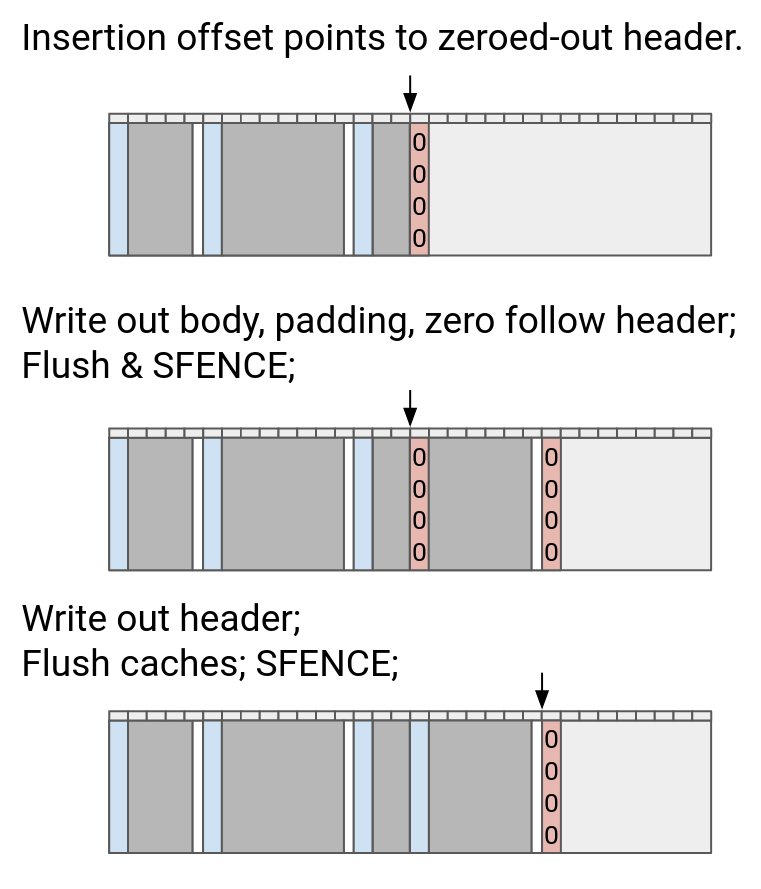
\includegraphics[trim=0cm 0.5cm 0cm 0.5cm,clip]{fig/prb_writepath_crashconsistent_append}
    \caption{
        The crash-consistent append operation to a PMEM chunk.
        The traversal algorithm reaches the existing entries at all times and reaches the new entry only after its body and header have been written completely.
    }
    \label{fig:prb_writepath_crashconsistent_append}
\end{figure}

The following implementation details of the append operation are relevant for latency and efficient use of CPU time:
\begin{itemize}[noitemsep]
    \item For ZIL-PMEM, the use of \lstinline{sfence} in phase 1 came with negligible impact on overall latency during development.
        We assume that this is because the wait time added by the \lstinline{sfence} is negligible compared to the write time for the entry body.
        For example, the entry body and zero padding for a 4k sync write is $sizeof(\mathtt{lr\_write\_t}) + data + padding = 4096 + 192 + 64 = 4352$ bytes large.
        Assuming 2~GiB/s write bandwidth for a single Optane DIMM~\cite{yangEmpiricalGuideBehavior2020}, the write time for the entry body is ca.~2~us.
        In contrast, the derived latency for a 256 byte write at that rate is ca.~0.12~us.
        If we use this value as an approximation for the cost of the \lstinline{sfence}, its latency contribution is only $\frac{0.12}{0.12 + 2} = 5.6\%$.
    \item All writes to PMEM happen in multiples of 256 bytes because 256 bytes is Optane's internal write unit size.
        Writes below this size cause read-modify-write cycles in the hardware and thus cost performance~\cite{yangEmpiricalGuideBehavior2020,zhangChameleonDBKeyvalueStore2021}.
    \item We use AVX-512 non-temporal store instructions (\lstinline{movnt}) instead of regular stores and cache flushes.
        Again, this addresses established performance properties of Intel Optane DC Persistent Memory~\cite{yangEmpiricalGuideBehavior2020}.
    \item We also use ZFS's optimized implementation of the Fletcher checksum to compute body and header checksums.
        Whereas the best implementation is chosen by benchmark dynamically at runtime, it is safe to assume that some SIMD ISA extension such as AVX-512 will be used if available.
    \item OpenZFS cannot rely on the Linux kernel's interface for saving FPU state due to licensing issues~\cite{LinuxCompatSIMD}.
        Unless the FPU is used by a dedicated kernel thread, ZFS must temporarily disable preemption, mask local interrupts, and manually save FPU state.
        PRB is written directly from the task that calls \lstinline{zil_commit} and thus incurs this overhead.
        We refactor ZFS's FPU state management abstraction so that FPU context is only saved once for both checksum computation and writing to PMEM.
        The time that is spent in this suboptimal state is bounded by the maximum log entry size.
        \todo{we have no evaluation on impact of interrupt masking, future work}
\end{itemize}

%Note that a fully sequential chain of entries is sufficient for today's ZIL since the commit list assembled by the ITX code\todo{ref} is already sequential.
%However, as pointed out by the example in the previous paragraph, full sequentiality is not always semantically necessary.
%This observation has already led to a prototype design for ZIL-LWB that allows for more parallel IO if the entries in written LWBs are not interdependent~\cite{openzfsZILPerformanceImprovements2020}.
%We interpret these findings as indicators that ZIL-PMEM --- and thus PRB --- should support parallelism on the write path in the form of diamond chains.
%We present an application of diamond chains to ZVOLs in Section~\ref{sec:itxgbypass} and evaluate it in Section~\ref{ch:eval}\todo{precise}.

%A generation is identified by its \textit{generation number} which is positive integer.
%An entry is always associated with exactly one generation but a generation can contain many entries.
%Entries within the same generation are identified through an \textit{id field} which is a positive integer.
%Given entries $a$ and $b$, $a \text{depends on} b \Leftrightarrow a.gen > b.gen$ where $x.gen$ denotes the generation of entry $x$.

\section{API Overview}\label{di:prb:api}
In this section, we briefly discuss the API of PRB/HDL that is consumed by the ZIL-PMEM ZIL kind.
In the implementation, most types and functions are prefixed with \lstinline{zilpmem_} or \lstinline{zilpmem_prb_t} which we omit for brevity.

\subsection{PRB Setup}
\begin{lstlisting}
prb_t* prb_alloc(size_t ncommitters);
void prb_free(prb_t *b, bool free_chunks);

chunk_t* chunk_alloc(uint8_t *pmem_base, size_t len);
void chunk_free(chunk_t *c);

void prb_chunk_initialize_pmem(chunk_t *c);
void prb_add_chunk(prb_t *prb, chunk_t *chunk);
\end{lstlisting}

The zpool import procedure allocates the PRB using the \lstinline{prb_alloc} function.
The returned \lstinline{prb_t} is owned by the caller which is responsible for freeeing it using \lstinline{prb_free} during pool export.

The PRB consumer allocates the chunk objects using \lstinline{chunk_alloc}.
It adds the chunk to the PRB using \lstinline{prb_add_chunk}.
The PRB assumes ownership of the chunks that are added to it.
When the PRB is constructed for the first time, the PRB consumer must call \lstinline{prb_chunk_initialize_pmem} to reset the PMEM sequence to an empty state.

The \lstinline{free_chunks} argument to \lstinline{prb_free} determines whether the PRB should free the chunks objects that were added to it, or whether the ownership moves back to the caller.
Note that freeing the chunk object (\lstinline{chunk_free}) does not alter the chunk's PMEM state.

\subsubsection{HDL Setup}\label{di:prb:api:hdl}
\begin{lstlisting}
void zil_header_pmem_init(zil_header_pmem_t *zh);
hdl_t* prb_setup_hdl(prb_t *prb, const zil_header_pmem_t *hdr);
void prb_teardown_hdl(hdl_t *hdl,
    bool abandon_claim, zil_header_pmem_t *upd);
\end{lstlisting}

HDLs recover their DRAM state from the ZIL header (\lstinline{zil_header_pmem_t}).
The setup \lstinline{prb_setup_hdl} function takes a constant pointer to the last-synced header.\todo{update impl}
The pointer is not internalized in HDL --- the pointee's lifetime may be as short as the function call.
The PRB consumer instantiates all dataset's HDLs during pool import or whenever a new dataset is created.
For new datasets, the initial value for the ZIL header (state \textit{nozil}) is set by \lstinline{zil_header_pmem_init}.

When the head dataset is destroyed or the pool is exported, the PRB consumer calls \lstinline{prb_teardown_hdl} to destroy the HDL.
The PRB must only be freed after all of its HDL's have been torn down.

\subsubsection{Claiming}\label{di:prb:api:claiming}

\begin{lstlisting}
check_replayable_result_t prb_claim(
    hdl_t *hdl, uint64_t pool_first_txg,
    zil_header_pmem_t *upd);
\end{lstlisting}
% NOTE: we omitted the whole claimstore stuff from the thesis because we rule out WR_INDIRECT support in the 'requirements' section.

After the PRB is constructed and HDLs are set up, we must \textit{claim} the log entries of all datasets' HDLs.
The corresponding function \lstinline{prb_claim} is invoked by the pool import procedure for each HDL.
The \lstinline{pool_first_txg} is the pool's first new transaction group.
For HDLs in state \textit{logging}, \lstinline{pool_first_txg - 1} becomes the $precrash\_txg$.

\lstinline{prb_claim} returns an update to the ZIL header through the \lstinline{upd} out-parameter.
We employ this pattern throughout the entire PRB API.
It is always the API consumer's responsibility to ensure that the update is correctly persisted in the correct transaction group.

Claiming can fail, e.g., if the procedure detects a missing entry for the HDL (claiming performs a dry-run of replay internally).
The API consumer defines the error handling policy.
It can either abort pool import or choose to abandon the log.
To abaondon the log, the API consumer must first tear down the HDL using \lstinline{prb_teardown_hdl(..., abandon_claim=true, ...)} to release claims made during \lstinline{prb_claim}.
Then, the API consumer can reset the ZIL header content using \lstinline{zil_header_pmem_init} and re-instantiate the HDL using \lstinline{prb_setup_hdl}.
The re-instantiated HDL is in state \textit{nozil}.
\todo{need third option to retry with an override flag that discards the unreplayable part of the log}

After all HDLs have been claimed the pool import procedure starts \textit{txg sync} which writes out the header updates made by claiming in the \lstinline{pool_first_txg}.
From that point on there is no need to coordinate HDL operations between different datasets.

% Remember from Section~\ref{bg:zfs:logreplay} that ZIL replay can be deferred for an indefinite amount of pool import/export cycles and system shutdowns.
% Claiming scans the PMEM chunks that were added with \lstinline{zilpmem_prb_add_chunk_for_claim} for log entries that need to be replayed.
% Chunks that contain unreplayed log entries are not considered when writing new entries.

\subsection{Replay}\label{di:prb:api:replay}

\begin{lstlisting}
typedef struct { ... } replay_result_t;

replay_result_t
prb_replay(hdl_t *hdl, replay_cb_t cb, void *cb_arg);

typedef struct replay_node replay_node_t;
typedef int (*replay_cb_t)(void *rarg,
    const replay_node_t *rn,
    const zil_header_pmem_t *upd);

typedef enum {
	READ_REPLAY_NODE_OK,
	READ_REPLAY_NODE_MCE,
	READ_REPLAY_NODE_ERR_CHECKSUM,
	READ_REPLAY_NODE_ERR_BODY_SIZE_TOO_SMALL,
} read_replay_node_result_t;

read_replay_node_result_t
prb_replay_read_replay_node(
    const replay_node_t *rn,
    uint8_t *body_out, size_t body_out_size,
    size_t *body_required_size);

void prb_replay_done(
    hdl_t *hdl, zil_header_pmem_t *upd);

\end{lstlisting}

When a dataset is mounted the mounting procedure must always call \lstinline{prb_replay}.
If the HDL is in state \textit{nozil}, the call is a no-op.
If the HDL is in state \textit{replaying}, the function invokes the provided replay callback for each log entry that needs to be replayed in replay order.
The callback must perform the following steps for crash-consistent replay for each replayed entry $E$.
\begin{enumerate}[noitemsep]
    \item Start a DMU transaction $tx$.
    \item Load the entry $E$ into a DRAM buffer using \lstinline{prb_replay_read_replay_node}.
    \item Apply the change encoded in $E$ to the dataset.
    \item Update the ZIL header to the value of \lstinline{*upd}.
    \item \lstinline{dmu_tx_commit(tx)} the DMU transaction.
\end{enumerate}

Note that the callback must use \lstinline{prb_replay_read_replay_node} function because \lstinline{replay_node_t} is an opaque type in the PRB API.
The function forces the API consumer to do DRAM buffering and protects against online and offline data corruption internally, as discussed in Section~\ref{di:prb:ccrecovery}.

\lstinline{prb_replay} can fail either due to an error returned by the callback, due to an error in the scanning phase, or due to log corruption.
If the error is due to missing log entries, the struct returned by the API contains the \textit{witness} log entry (see Section~\ref{di:prb:deptrack}).
The caller decides whether to retry replay or abandon the remaining unreplayable part of the log\todo{retry with an override flag that discards the unreplayable part of the log}.
End of replay must be acknowledged explicitly by calling \lstinline{prb_replay_done}.
Abandoning the log is done using \lstinline{prb_destroy_log} (next section).

%The invocation order corresponds to the order in which the entries were written.
%Entries that were written in parallel (\lstinline{needs_new_gen == false}) are replayed in a deterministic order to allow for resumability.

\subsection{Writing Entries}\label{di:prb:api:write}

\begin{lstlisting}
bool prb_create_log(hdl_t *hdl, zil_header_pmem_t *upd);
void prb_destroy_log(hdl_t *hdl, zil_header_pmem_t *upd);

int prb_write_entry(hdl_t *hdl,
    uint64_t txg, bool needs_new_gen,
    size_t body_len, const void *body_dram);
\end{lstlisting}

After successful replay, the HDL is always in the unwritable state \textit{nozil}.
The log writer must use \lstinline{prb_create_log} to create a new log idempotently.
If the HDL is in state \textit{nozil}, the function allocates a log GUID and transitions the HDL to state \textit{logging}.
Otherwise, the HDL must already be in state \textit{logging} and the call is a no-op.
If a new log was created, the caller must ensure that the transaction group that persists the ZIL header update has synced to disk before starting to write log entries.
The caller distinguishes the cases based on the function's return value.

Log writers use the \lstinline{prb_write_entry} function to write log records to the HDL.
The log record is treated as an opaque blob.
PRB does not provide facilities to version different version of the encoding.\todo{should we? future work}
In addition to the body (\lstinline{body_dram}, \lstinline{body_len}), the log writer must provide two pieces of metadata:
\begin{description}[noitemsep,leftmargin=1.5cm,labelindent=1cm]
    \item[txg] The transaction group $T_{i_{txg}}$ of the DMU transaction $T_i$ whose changes $C_i$ are encoded in the log entry.
        Note: for ZIL-PMEM, this value is always the same as the log record's \lstinline{lrc_txg} field.
    \item[needs\_new\_gen] Indicates whether a new generation should be started for this log entry.
        It is the responsibility of the caller to serialize the start of a new generation as described in Section~\ref{di:prb:write:hdlscoped}.
        If a thread writes an entry with \lstinline{needs_new_gen} is \lstinline{true}, that thread must be the only thread executing \lstinline{zilpmem_prb_write_entry} for the given HDL.
        The contrary is not true: if \lstinline{needs_new_gen} is \lstinline{false}, multiple threads may write entries in parallel to the same HDL.
        Note that writers for different HDLs do not need to coordinate at all.
\end{description}

\subsubsection{Garbage Collection}

\begin{lstlisting}
void prb_gc(prb_t *prb, uint64_t synced_txg);
\end{lstlisting}

Whenever \textit{txg sync} has finished syncing a txg $T$ to the main pool it must call \lstinline{prb_gc} with \lstinline{synced_txg = T}.
Note that unlike writing or recovering an individual log, garbage collection is a PRB-level operation.
Synchronization is handled internally.

% \subsubsection{ZIL header}\label{di:prb:persistent:zilheader}
% The ZIL header (\lstinline{zil_header_pmem_t}) is the persistent representation of the HDL state.
% Not every aspect of the runtime state of HDL is reflected in it, but only the information needed for claiming and replay.
% The ZIL header has the following states, some of which have associated data:
% \begin{description}[noitemsep,leftmargin=1.5cm,labelindent=1cm]
%     \item[nozil] There is no log for this dataset. (No associated data.)
%     \item[logging] The log has been created and entries might have been written to PMEM.
%         Claiming has never been attempted or never been completed.
%         The log remains in this state for the entire time until it is destroyed or the system crashes. Associated data: \textit{Log GUID}.
%     \item[replaying] The log has been claimed and replay is ongoing. Associated data: \textit{Log GUID} and \textit{serialized replay algorithm state}.
% \end{description}
% The diagram in Figure~\ref{fig:prb_persistent_structure__header_states_plus_example} visualizes the state transitions that the ZIL header goes through as the log is created, written and recovered.

% \begin{figure}
%     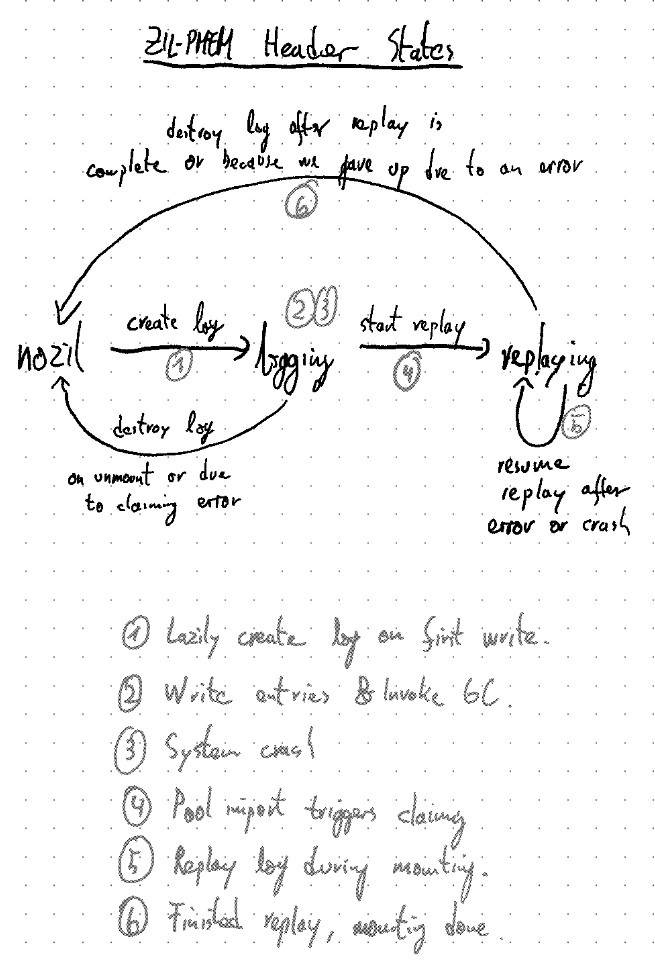
\includegraphics[height=15cm]{fig/prb_persistent_structure__header_states_plus_example}
%     \caption{
%         The states of \lstinline{zil_header_pmem_t} and the events that cause state transitions.
%         The grey annotations illustrates the path from log creation to finished recovery.}
%     \label{fig:prb_persistent_structure__header_states_plus_example}
% \end{figure}

% We use the following C structure to encode the ZIL header state.
% The \lstinline{zhpm_st} field is always valid and is one of \lstinline{ZHPM_ST_NOZIL}, \lstinline{ZHPM_ST_LOGGING}, or \lstinline{ZHPM_ST_REPLAYING}.
% The \lstinline{zhpm_guid_} fields are only valid in states \lstinline{ZHPM_ST_LOGGING} and \lstinline{ZHPM_ST_REPLAYING}.
% The \lstinline{zhpm_replay_state} is only valid in state \lstinline{ZHPM_ST_REPLAYING}.
% Hence we will describe its contents in Section~\ref{di:prb:recovery}.
% \begin{lstlisting}
% typedef enum zil_header_pmem_state {
%     ZHPM_ST_NOZIL,
%     ZHPM_ST_LOGGING,
%     ZHPM_ST_REPLAYING,
% } zil_header_pmem_state_t;

% typedef struct zil_header_pmem {
%     uint64_t zhpm_st; /* zil_header_pmem_state_t */
%     uint64_t zhpm_guid_1;
%     uint64_t zhpm_guid_2;
%     zilpmem_replay_state_phys_t zhpm_replay_state;
% } zil_header_pmem_t;
% \end{lstlisting}





% \subsubsection{Replay Sequence Algorithm}
% The basis for claiming and replay is the \textit{replay sequence algorithm}.
% Its inputs are the HDL's log GUID, a set of \lstinline{prb_chunk_t} references, and a callback.
% The algorithm consists of a \textit{scanning phase} and an \textit{iteration phase}.
% The scanning phase uses the traversal algorithm (Section~\ref{di:prb:traversal}) to search for log entries that have the HDL's \textit{log GUID} in all chunks that are provided as input.
% It wraps each of these candidate entries in a \textit{replay node} and collects the nodes in a b-tree.
% In the \textit{iteration phase}, the algorithm \textit{visits} each replay node by iterating over the b-tree.
% For each node, it checks whether the corresponding entry still needs to be replayed and if so, invokes the provided callback.

% The \textit{replay node} stores the following metadata about an entry:
% \begin{description}[noitemsep,leftmargin=1.5cm,labelindent=1cm]
%     \item[Generation (gen)] The entry's generation.
%     \item[Generation-Scoped ID (gsid)] The entry's generation-scoped ID.
%     \item[PMEM Address] The start address of the entry in PMEM.
%     \item[Transaction Group (txg)] The entry's transaction group.
%     \item[Counter Table] The counter table stored in the entry.
%     \item[Pointer To Chunk (chunk\_ref)] A pointer to the \lstinline{prb_chunk_t} that contains the entry.
% \end{description}
% The replay nodes of a well-formed HDL log are uniquely identified by $(gen, gsid)$.
% %The b-tree identifies and sorts replay nodes by $(gen, gsid)$ in element-wise ascending order.
% The lexicographical ordering of that tuple is the replay ordering, and also the ordering used in the b-tree.
% For example, the replay nodes $(2,1), (1,1), (1,3)$ are visisted in order $(1,1), (1,3), (2,1)$.

% \begin{samepage}
% The iteration phase iterates over the replay nodes in the b-tree in the order defined above.
% It maintains the following state variables and executes the subsequently listed steps for each visisted replay node $N$:
%  \begin{description}[noitemsep,leftmargin=1.5cm,labelindent=1cm]
%     \item[precrash-txg] The last txg that finished syncing out before the system crashed.
%     \item[$\mathbf{(gen_{last}, gsid_{last})}$] The $gen$ and $gsid$ of the last replay node that was visited.
%         A value of $(0,0)$ means that no replay node has been visited yet.
%     \item[validating counter tables] A \textit{live} and \textit{last} table; same layout as used on the write path (see Section~\ref{di:prb:write:logstructureencoding}).
% \end{description}
% % The following rules determine whether the callback is invoked for a replay node $N$:
% % Remember that $E$ for generation $E.gen$ depends on all entries in all generations $gen < E.gen$.
% % Also remember that $E$ must only be replayed if the changes of its transaction group $E.txg$ have not been applied to the dataset.
% Steps per node $N$:
% \begin{enumerate}[noitemsep]
%     \item \label{replayStep:skiptxg} Skip $N$ if its $N.txg \le precrash\_txg$.
%     \item \label{replayStep:skipreplayed} Skip $N$ if $(N.gen,N.gsid) \le (gen_{last}, gsid_{last})$.
%     \item \label{replayStep:validate} Compare the validating \textit{last table}'s counters to the Counters Table stored in $N$.
%         We only compare counters for $txg > precrash\_txg$.
%         Proceed iff the counters match. Otherwise, stop the iteration, and return $N$ as a \textit{witness} for log corruption.
%     \item \label{replayStep:bump1} If $N.gen \neq gen_{last}$, compute a new validating \textit{last table} from the validating \textit{live table}.
%     \item \label{replayStep:bump2} Increment the validating \textit{live table}'s counter for txg $N.txg$.
%     \item \label{replayStep:bump3} Update $(gen_{last}, gsid_{last}) = (N.gen, N.gsid)$.
%     \item \label{replayStep:invoke} Invoke the callback provided by the algorithm's consumer, passing $N$ as an argument.
%         If the callback returns an error, rollback the update to $(gen_{last}, gsid_{last})$ and the counter tables, stop the iteration, and return.
%         Otherwise, proceed to the next replay node.
% \end{enumerate}
% \end{samepage}
% Step~\ref{replayStep:skiptxg} filters out entries whose changes had already been synced to the pool before the system crashed.
% Step~\ref{replayStep:skipreplayed} filters out entries for which the callback has already been invoked.
% Comparing the counters in step~\ref{replayStep:validate} ensures that no entries in generations $gen < N.gen$ and $txg > precrash\_txg$ have been lost.
% These are precisely the entries that $N$ logically depends on (Section~\ref{di:prb:structure}).
% Steps~\ref{replayStep:bump1} and \ref{replayStep:bump2} then ensure that step \ref{replayStep:validate} will pass for entries in later generations, their $(gen, gsid) > (N.gen, _)$ unless later entries have been lost.
% And \ref{replayStep:bump3} ensures that $N$ is going to be skipped by step~\ref{replayStep:skipreplayed} in the future and thus will not be double-counted by steps~\ref{replayStep:bump1} and \ref{replayStep:bump2}.

% The iteration phase has a number of important properties (no proof):
% \begin{enumerate}[noitemsep]
%     \item If no entries are missing, the callback is invoked exactly once for each replay node whose log entry needs to be replayed.
%         The invocation order is the replay order (= lexicographical order of $(gen, gsid)$).
%         Thus, the logical dependencies of each entry for which the callback is invoked are expected.
%     \item If a log entry is missing in generation $gen_l$, we still invoke the callback for all other entries within $gen_l$.
%         If step~\ref{replayStep:validate} finds a witness $(gen_w, \_)$ for a missing entry, it is guaranteed that th $gen_w > gen_l$.
%         This behavior correct and desirable because by definition, entries within a generation have no logical dependency on each other.
%     \item The previous property is particularly important for parallel logging to the same HDL:
%         if multiple threads write entries to a HDL's open generation in parallel, any entry that finished writing before the system crashes will be replayed, even if other threads had not finished writing before the crash.
%     \item Loss of entries at the tail of the logical log cannot be detected because there is no record of their existence in prior log entries.
%         Note that this is the status quo with ZIL-LWB as well, both with and without OpenZFS Native Encryption.
%     \item The iteration phase correctly handles \textit{online} data corruption in PMEM, i.e., data corruption while the iteration is running.
%         The reason is that we operate on DRAM-buffered copies of the entry metadata in the replay node, and force the callback to use the \lstinline{prb_replay_read_replay_node} function to access the entry.
%         The function copies the entry to PMEM using \lstinline{memcpy_mcsafe}, revalidates the checksums, and esnures that the entry metadata still matches the replay node.
%     \item The iteration phase can be checkpointed by snaphotting its state variables from within the callback invocation for a replay node $N_{cp}$.
%         The replay sequence algorithm can be restarted from the checkpointed state by re-executing the \textit{scanning phase} and restoring the iteration state variables from the checkpoint.
%     \item The restarted algorithm behaves exactly as if the callback invocation for $N_{cp}$ had returned without error.
%         All of the properties above hold for the for the restarted aI.e., all of the already replayed entries are skipped in step~\ref{replayStep:skipreplayed}, including $N_{cp}$.
%     \item All properties listed above hold for across resume from checkpoints.
%         \begin{itemize}
%             \item Loss of entries $N_{l} \le N_{cp}$ does not affect the behavior of the restarted algorithm.
%             \item Loss of entries $N_{l} > N_{cp}$ affects the behavior the same way as without checkpointing.
%         \end{itemize}
%         \item Data corruption in entries that would be skipped, their $(gen, gsid) <= (gen_{last}, gsid_{last})$ does not 
%         Loss of entries $ \le N_{cp}$ does not affect the behavior of the restarted algorithm.
%         \item Loss of entries $N_{l} > N_{cp}$ affects the behavior the same way as without checkpointing.
%     \end{enumerate}
% We provide examples for counter table validation in Figure~\ref{todo}.

% The iteration phase can be checkpointed by snaphotting the state variables from within the callback.
% Restarting the iteration from the checkpointed state causes all replay nodes for which the callback had already been invoked to be skipped.
% Replay relies on this feature for crash-tolerance: for every invocation of the replay callback, it both applies the change encoded in the log entry and persists the checkpointed iteration state to the ZIL header.
% By performing these changes in the same DMU transaction, the effect of the change and the checkpoint are persisted to the main pool atomically.
% If the system crashes and replay restarts from the checkpointed state, it skips exactly all changes that have already been applied.

% The replay sequence algorithm is resilient against random \textit{online} data corruption in PMEM, i.e., data corruption while the algorithm executes.
% The reason is that both phases only operate on DRAM-buffered copies of the entry metadata in the replay node.
% Further, if the callback needs to read the entry, our API forces it to use DRAM-buffering as well:
% it does not receive a pointer into PMEM but a pointer to the (opaque) replay node struct.
% To copy the entry into a DRAM buffer, it must use the \lstinline{prb_replay_read_replay_node} function which
% \begin{itemize}[noitemsep]
%     \item handles machine-check exceptions (MCEs) through \lstinline{memcpy_mcsafe},
%     \item validates the header and body checksums of the entry, and
%     \item ensures that the metadata cached in the replay node did not change since the scanning phase.
% \end{itemize}

% \subsubsection{Claiming}
% The claiming phase during pool import (\lstinline{zilpmem_prb_claim}) uses the \textit{replay sequence algorithm} to find the set of chunks that contain entries of the log that is being claimed.
% This set of chunks is stored in DRAM inside the HDL for later use by replay.
% We refer to it as the HDL's \textit{claimset}.

% The set of chunks that claiming provides as input are the chunks on the \textit{wait replay list} which was filled by \lstinline{zilpmem_prb_add_chunk_for_claim} during PRB construction (Section~\ref{prb:di:chunkownership}).
% The claiming callback performs the following steps for each replay node $N$ for which it is invoked:
% \begin{enumerate}[noitemsep]
%     \item Add the chunk $N.chunk\_ref$ to the HDL's claimset.
%         If the chunk was not yet included in the set, increment the chunk's \textit{claim refcount} (Section~\ref{prb:di:chunkownership}).
%     \item Check for PMEM corruption by reading the log entry from PMEM using \lstinline{prb_replay_read_replay_node}.
% \end{enumerate}
% If log corruption is detected by the replay sequence algorithm or the callback, we fail the pool import operation.
% In that case, the \textit{claim refcount}s are decremented during HDL teardown.
% \todo{in the impl, we currently panic on error because we'd need to change how import works. It's just a bunch of engineering work, not relevant for the thesis.}
% Otherwise, if no errors have occured, the HDL transitions into a state where it waits for replay.

% Claiming is responsible for transitioning the ZIL header from \textit{logging} to \textit{replaying} when the log is first claimed after a crash.
% It initializes the associated \lstinline{zilpmem_replay_state_phys_t} value which contains the checkpointed iteration state used by replay.
% The value for $precrash\_txg$ is the pool's first transaction group that will be synced once txg sync starts.
% $(gen_{last}, gsid_{last})$ is $(0, 0)$.
% All rows in the \textit{validating counter tables} are invalidated by setting their $txg$ to $0$.

% Note that the transition of the ZIL header from \textit{logging} to \textit{}only occurs once for every log.
% If the system crashes and we claim we claim 
% If the ZIL header is already in state \textit{replaying} when c the checkpointed iteration state is simply restored to DRAM.

% \subsubsection{Replay}
% % reconstructs replay sequence, only scans HDL's held chunks list
% % explain how replay stores its state in a struct
% % state is serialized and passed replay callback for DMU transaction
% % explain how crash during replay and resume works
% Replay (\lstinline{zilpmem_prb_replay}) uses the replay sequence algorithm to recover dataset state.
% Remember from Section~\ref{di:prb:api:replay} that \lstinline{zilpmem_prb_replay} itself receives a callback $C_{consumer}$ from the API consumer.
% The API contract states that $C_{consumer}$ receives the replay node and an updated version of the ZIL header as arguments.
% It must, in one DMU transaction, replay the change encoded in the replay node's entry and apply the ZIL header update.
% This makes \lstinline{zilpmem_prb_replay} is a thin wrapper around the replay sequence algorithm.
% The set of chunks to be traversed by the algorithm is the \textit{claimset} that the claiming procedure stored in the HDL.
% A thin wrapper callback $C_{wrapper}$ translates from the replay sequence algorithm's limited view on replay to the HDL-wide view of the replay API.
% $C_{wrapper}$ receives the replay node $N$ as an argument. It performs the following steps:
% \begin{enumerate}
%     \item Compute the new ZIL header $H_{new}$ from the HDL state.
%         The replay sequence algorithm already updated the replay state before invoking the callback, thus $H_{new}$ will contain the updated \lstinline{zilpmem_replay_state_phys_t}.
%     \item Invoke $C_{consumer}(N, H_{new})$ and return its return value.
% \end{enumerate}

% Our solution is to externalize all of the iteration phase's state into the \lstinline{zilpmem_replay_state_t} structure.
% The \lstinline{zilpmem_replay_state_t} is the dirty in-DRAM copy of the on-disk \lstinline{zilpmem_replay_state_phys_t} which is stored in the ZIL header (Section~\ref{di:prb:persistent:zilheader}).
% It is the responsibility of claiming and replay to keep the two in sync.
% After a system crash during claiming or replay, the HDL setup routine recovers the in-DRAM state from the last-synced on-disk state in the ZIL header.
% The replay sequence algorithm is thus unaware of the crash.

% This is necessary when the algorithm is used by replay: the callback provided by replay persists the iteration phase's state to the ZIL header.


\chapter{Integration into ZFS}\label{ch:zilpmem}
In this chapter we describe how we integrate PRB/HDL into ZFS in three steps.
First, in Section~\ref{ch:zilkinds}, we describe how we re-architect ZFS to support different ZIL implementations (\textit{ZIL Kinds)} at runtime (Section~\ref{ch:zilkinds}).
Then, in Section~\ref{sec:pmemspavdev}, we present our approach to make ZFS's device management layer (VDEV) aware of persistent memory devices.
Finally, in Section~\ref{sec:zilpmemzilkind}, we describe how we combine PRB/HDL and PMEM SLOG VDEVs into the new \textit{ZIL-PMEM} ZIL kind.

\section{ZIL Kinds}\label{ch:zilkinds}
Coexistence with the existing ZIL and preservation of ZFS's crash consistency guarantees are two requirements for ZIL-PMEM (see Section~\ref{sec:requirements}).
Our solution to both of these problems is to re-architect ZFS to support different persistence strategies for the ZIL while sharing all code and data structures that ultimately define crash consistency semantics.
In order to make the integration of ZIL-PMEM seamless to the end user (goal: simple administration), the persistence strategy is the same for all datasets in a pool.
The variable that determines the pool's persistence strategy is its \textit{ZIL kind}.
The following sub-sections present how we refactor ZFS to support ZIL kinds.
The existing ZIL, which uses LWBs for persistence (cf. Section~\ref{ch:openzfs_background:zillwb_persistence}) becomes the first ZIL kind called \textit{ZIL-LWB}.
Note that some listings and figures in this section already mention ZIL-PMEM.
However, in our implementation, all refactoring steps presented in this section are separate commits that precede the introduction of the ZIL-PMEM ZIL kind.

\subsection{On-Disk State}\label{sec:di:zil_header}
ZIL-LWB keeps its state in the ZIL header which is stored in the \lstinline{objset_phys_t} structure.
For ZIL kinds, we change the ZIL header to be a tagged union that uses the new \lstinline{zh_kind_t} enum as a discriminant.
The existing ZIL-LWB header fields are moved into the \lstinline{zil_header_lwb_t} type.
ZIL-PMEM's ZIL header, which we describe in Section~\ref{ch:zilpmem}, is the second member of that union.
Figure~\ref{lst:zil_header_before_and_after} shows the relevant C structures before and after the changes described in this paragraph.

\begin{figure}[H]
\begin{subfigure}[t]{0.45\textwidth}
\begin{lstlisting}[basicstyle=\scriptsize\ttfamily]
typedef struct zil_header {
  uint64_t zh_claim_txg;
  uint64_t zh_replay_seq;
  blkptr_t zh_log;
  uint64_t zh_claim_blk_seq;
  uint64_t zh_flags;
  uint64_t zh_claim_lr_seq;
  uint64_t zh_pad[3];
} zil_header_t;
\end{lstlisting}
\end{subfigure}
\hfill
\begin{subfigure}[t]{0.5\textwidth}
\begin{lstlisting}[basicstyle=\scriptsize\ttfamily]
typedef enum {
  ZIL_KIND_UNINIT,
  ZIL_KIND_LWB,
  ZIL_KIND_PMEM,
  ZIL_KIND_COUNT
} zh_kind_t;

typedef struct zil_header_lwb {
  /* fields of zil_header_t,
   * without zh_pad */
} zil_header_pmem_t;

typedef struct zil_header_pmem {
  /* introduced later */
} zil_header_pmem_t;

typedef struct zil_header {
  union {
    zil_header_lwb_t zh_lwb;
    zil_header_pmem_t zh_pmem;
  };
  uint64_t zh_kind;
  uint64_t zh_pad[2];
} zil_header_t;

\end{lstlisting}
\end{subfigure}
\caption{The ZIL header structs (in DRAM and on disk) before and after the introduction of ZIL kinds. Note that we carve out the space for \lstinline{zh_kind} from \lstinline{zh_pad[3]} which is guaranteed to be zeroed.}
\label{lst:zil_header_before_and_after}
\end{figure}

\subsubsection{Compatibility}

We register ZIL kinds as a \textit{zpool feature} flag.
Feature flags are OpenZFS's mechanism for expressing variants of the on-disk format.

Whenever we access the ZIL header, we first check the activation status of the feature flag.
If the feature is not active, we implicitly know that the ZIL kind is ZIL-LWB and always access \lstinline{zh_lwb}.
If the feature is active, we use the \lstinline{zh_kind} discriminant field to determine the ZIL kind.

ZIL kind implementations only access their sub-structure within the ZIL header.
For example, ZIL-LWB only operates on the \lstinline{zil_header_lwb_t} structure, not the full \lstinline{zil_header_t}.
Hence, there is no difference to the ZIL-LWB implementation whether ZIL kinds are enabled or not.

The migration path for activating ZIL kinds is simple since all ZIL headers in the pool are guaranteed to be ZIL-LWB before the migration.
The only change is to set \lstinline{zh_kind = ZIL_KIND_LWB} for all ZIL headers.
(We found the \lstinline{ZIL_KIND_UNINIT} variant, which is the zero value, to be very helpful in catching initialization bugs and would not want to miss it.)

New ZIL kinds, such as ZIL-PMEM, will require their own \textit{zpool feature}s that are marked as dependent on the ZIL kinds feature.
However, this is not a solution for decentralizing the assignment of new \lstinline{zh_kind_t} enum variants to identify ZIL kinds in \lstinline{zh_kind}.
We have not yet come to a satisfying solution for this problem.

\subsection{Runtime State}\label{sec:zil_kinds:runtime}
In upstream ZFS, the ZIL runtime state is kept in the per-dataset \lstinline{zilog_t} object.
\lstinline{zilog_t} holds the \textit{itxg} structure that is used to track uncommitted ITXs.
\lstinline{zil_commit} drains the ITXs into the \textit{commit list} and proceeds by packing their encoded representation (log records) into LWBs.
(See Section~\ref{openzfs:the_zil_api} and \ref{ch:openzfs_background:zillwb_persistence} for details.)

We observe the following properties of the upstream ZIL code:
\begin{itemize}[noitemsep]
    \item The \textit{itxg} data structure defines the framework for ZFS's crash consistency semantics.
          Whereas ZPL and ZVOL code create the ITXs, the organization by \lstinline{itxgs} and the code that assembles the commit list constraints what can be expressed in them.
    \item ITXs and even the commit list are independent of the LWB chain that is ultimately written to disk.
          The commit list merely defines the set and order of ZIL records that need to be persisted to some form of sequential log.
    \item The interface between the ITX- and LWB-related code is limited to the \textit{commit list} and its contents.
        The responsibilities are thus already (conceptually) separated.
\end{itemize}
Given these insights we refactor the ZIL implementation (\textit{zil.c}) as follows:
\begin{enumerate}[noitemsep]
    \item Move all non-ITX functions into a separate module \textit{zil\_lwb.c} and prefix them with \lstinline{zillwb_}.
          If the function was part of the public ZIL API, add a wrapper function with the original name to \textit{zil.c} that forwards the call to the \lstinline{zillwb_} function in \textit{zil\_lwb.c}.
    \item Virtualize calls to \lstinline{zillwb_} functions in \textit{zil.c}:
          \begin{itemize}
              \item Define a struct \lstinline{zil_vtable_t} that contains function pointers with the type signature of each of the \lstinline{zillwb_} functions called from \textit{zil.c}.
              \item Define \lstinline{zillwb_vtable} as an instance of \lstinline{zil_vtable_t} that uses \lstinline{zillwb_} functions as values for the respective function pointer members.
              \item Add a member \lstinline{zl_vtable} to \lstinline{zilog_t} that is pointer to a \lstinline{zil_vtable_t}.
              \item Replace all calls to \lstinline{zillwb_FN()} in \textit{zil.c} with indirect calls through the vtable, i.e., \lstinline{zilog->zl_vtable.FN()}.
          \end{itemize}
    \item Make non-ITX state private to \textit{zil\_lwb.c} by turning it into a sub-object.
          \begin{itemize}
              \item Move the \lstinline{zilog_t} members that are only used by the functions in \textit{zil\_lwb.c} into a separate structure called \lstinline{zilog_lwb_t} that is private to \textit{zil\_lwb.c}.
              \item Embed \lstinline{zilog_t} as the first member in \lstinline{zilog_lwb_t}.
              \item Add member \lstinline{zlvt_alloc_size} to \lstinline{zl_vtable_t} that indicates the amount of memory to be allocated when allocating a \lstinline{zilog_t}.
              \item Add a \textit{downcast} step to the start of each \lstinline{zillwb_} functions that casts the \lstinline{zilog_t} pointer into a \lstinline{zilog_lwb_t} pointer.
                The cast is safe because \lstinline{zilog_t} is embedded as the first member of \lstinline{zilog_lwb_t}.
                The majority of \lstinline{zillwb_} functions operate only on the \lstinline{zilog_lwb_t}-private state without accessing the embedded \lstinline{zilog_t}.
              \item Add constructor and destructor methods to the vtable that are called after allocating the \lstinline{zlvt_alloc_size}d \lstinline{zilog_t}.
                The \lstinline{zillwb_} constructor and destructors initialize and deinitialize the private members of \lstinline{zilog_lwb_t}.
          \end{itemize}
\end{enumerate}
The end result ist best described in the terminology of object-oriented programming:
\textbf{\lstinline{zilog_t} is an abstract base class} that implements the public ZIL interface as well as ITX-related functionality and defines abstract methods for persisting log records.
These abstract methods must be implemented by concrete subclasses.
\lstinline{zilog_lwb_t} is such a subclass that implements the LWB-based persistence strategy.
For ZIL-PMEM, the \lstinline{zilog_pmem_t} struct which we introduce in Section~\ref{ch:zilpmem} implements persistence directly to PMEM.
Which subclass is instantiated at runtime is determined by the \lstinline{zh_kind} field in the ZIL header.
Figure~\ref{fig:zilog_splitup_viz} illustrates the changes described in this section.

\begin{figure}[H]
    \centering
    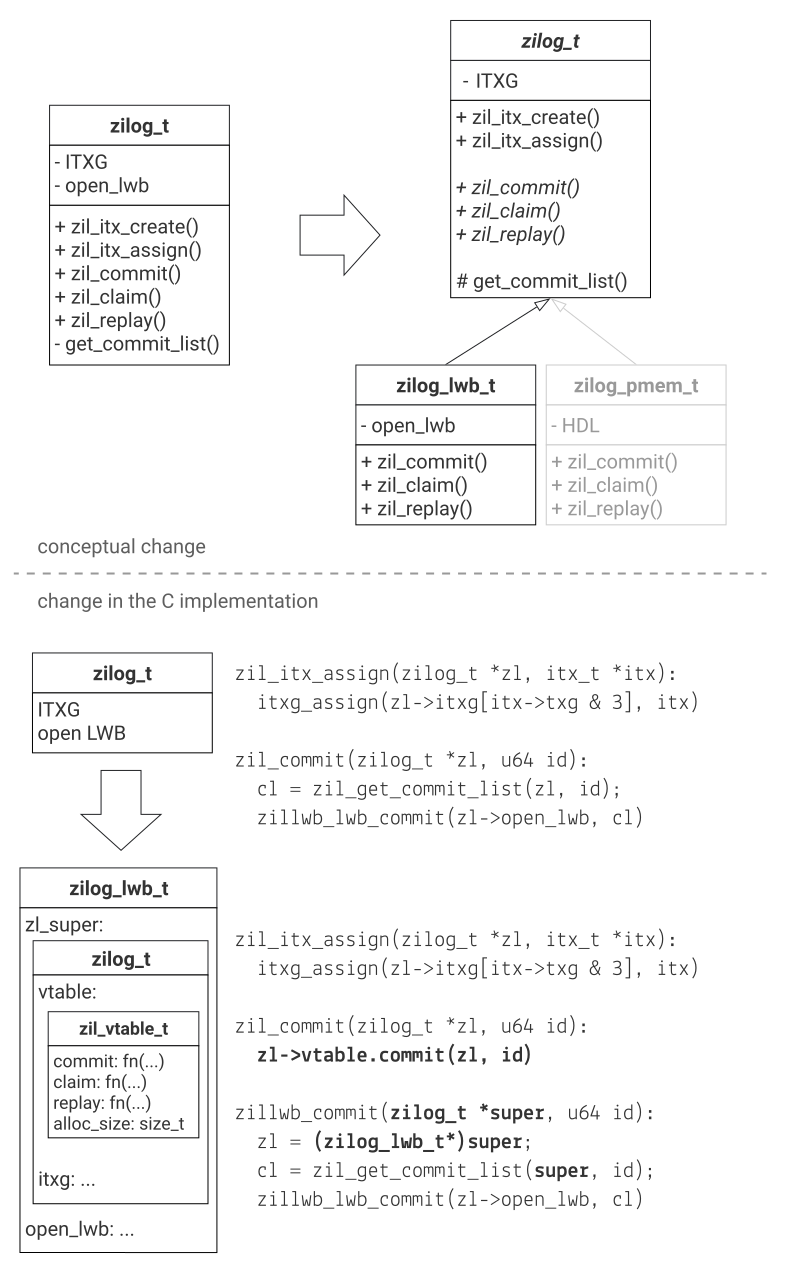
\includegraphics{fig/zilog_splitup_viz}
    \caption{\lstinline{zilog_t} before and after the introduction of ZIL kinds by example of the \lstinline{zil_itx_assign()} and \lstinline{zil_commit()} APIs.}
    \label{fig:zilog_splitup_viz}
\end{figure}


\subsection{Changing ZIL Kinds}\label{sec:zil_kinds:change}
%The following steps must happen in the same transaction group as the SLOG addition or removal that triggers the change of ZIL kind:
A zpool's ZIL kind can be changed by atomically switching over the \lstinline{zh_kind} of every ZIL header in the pool.
The following procedure enables online switching of the ZIL kind:
\begin{enumerate}[noitemsep]
    \item Ensure that all dataset's ZILs have been replayed. If not, cancel the procedure unless the caller specified to drop unreplayed logs.
    \item Stop use of the ZIL API and wait until all active API calls to it have finished.
    \item Wait for all ZIL entries to become obsolete by waiting for the current open txg to be synced.
    \item Free all dataset's \lstinline{zilog_t} instances.
    \item \label{changezilkinds:switchheaders} Set all datasets' ZIL headers to the new ZIL kind's default value.
        The default value is the ZIL state that encodes the absence of log entries, e.g., \textit{nozil} for ZIL-PMEM.
    \item Allocate the new \lstinline{zilog_t} instances and bring them into a usable state.
        The allocation routine uses \lstinline{zh_kind} to select the (new) vtable, allocates \lstinline{zlvt_alloc_size} bytes for the new \lstinline{zilog_KIND_t} and runs the ZIL kind specific constructor.
    \item Re-allow use of the ZIL API.
\end{enumerate}
Step~\ref{changezilkinds:switchheaders} must happen atomically for all ZIL headers in the pool.
Otherwise, a crash could result in a pool with mixed ZIL kinds.

Due to time constraints we have \textbf{not yet implemented} the procedure outlined above.
As a stop-gap solution, we instead implemented a simplified scheme where a zpool's ZIL kind is determined on pool creation time by a kernel module parameter (\lstinline{zil_default_kind}).
On subsequent pool imports, we derive the pool's ZIL kind from the root dataset's ZIL kind.
We prevent attempts to switch the ZIL kind by preventing any changes to the SLOG VDEV config in a ZIL-PMEM pool.

% DON'T point out that the design alternative is to have internal polymorphism within zilog_t. It's trivial to see from an implementor's perspective.

\subsection{ZIL-LWB Suspend \& Resume}\label{sec:zil_kinds:suspend_resume}
The ZIL API provides the \lstinline{zil_suspend} and \lstinline{zil_resume} functions.
\lstinline{zil_suspend} halts all ZIL activity and waits until all log entries are obsolete before returning to the caller.
\lstinline{zil_resume} reverts the state to normal operation.
Compatibility code for versions of ZFS prior to the \textit{fast snapshots} feature rely on ZIL suspend \& resume for taking snapshots.
For newer pool versions, the only consumer is \lstinline{spa_reset_logs}: when removing a SLOG from the pool, the ZIL is temporarily suspended to ensure that the SLOG does not contain valid log entries.
After the SLOG is removed, the ZIL is resumed and the SPA uses the remaining SLOGs or the main pool devices to allocate LWBs.

With regard to ZIL kinds, only the \lstinline{spa_reset_logs} use case is relevant since ZIL kinds require a more recent pool version than the \textit{fast snapshots} feature.
Our design for changing ZIL kinds (Section~\ref{sec:zil_kinds:change}) requires suspension of all ZIL activity and thus subsumes the ZIL-LWB specific \lstinline{zil_suspend} and \lstinline{zil_resume}.
However, the compatibility code for pools before \textit{fast snapshots} needs to be maintained in a way that does not depend on the ZIL kinds feature.
Due to time constraints, we were \textbf{unable to address suspend \& resume in our design}.
We expect that the solution will be highly dependent on implementation-level constraints.

\subsection{ZIL Traversal \& ZDB}\label{sec:zil_kinds:traversal}
Whereas ZIL writing and replay are abstracted away by the \lstinline{zilog_t} refactoring, there are several cases where the raw ZIL-LWB chain is traversed directly using the \lstinline{zil_parse} function.
\lstinline{zil_parse} exposes several ZIL-LWB specific implementation details to its callers such as blockpointers and the concept of LWBs.
This is problematic for ZIL kinds because not every conceivable ZIL kind uses these concepts --- ZIL-PMEM being the obvious example.
We investigate all users of the ZIL traversal code and come to the conclusion that there is no need for a generalized interface that every ZIL kind needs to implement.
The basis for this decision is a manual audit of all \lstinline{zil_parse} callers:
\begin{description}[noitemsep]
    \item[dmu\_traverse] This code module implements a callback-based traversal of the zpool's data structures.
    It is used to implement many ZFS features, e.g., \mbox{\textit{zfs send}}.
    If a dataset is traversed that is a head dataset and its LWB chain has been claimed, the LWBs are included in the traversal.
    (In the previous sentence, ``claimed'' refers to ZIL-LWB's claiming, not ZIL-PMEM's.)
    \item[dsl\_scan\_zil] During a \textit{zpool scrub} (data integrity check of the entire pool), this function traverses claimed LWB chains.
    \item[spa\_load\_verify] During pool import this function uses \textit{dmu\_traverse} to validate data structures that were modified in the last synced transaction groups.
    \item[zdb\_il.c] The \textit{ZFS debugger} interprets the ZIL header of head datasets, traverses their LWB chain, and dumps its contents to stdout.
\end{description}
Most consumers of \textit{dmu\_traverse} operate on snapshots, not head datasets, and therefore do not trigger ZIL chain traversal.
The \textit{dsl\_scan} and \textit{spa\_load} code only traverses the ZIL but does not access its data --- the data integrity checks that are done for validation are implemented transparently in the ZIO read pipeline that is used to load the LWBs in the ZIL chain.
One compatibility code path (\lstinline{old_synchronous_dataset_destroy}) uses \lstinline{dmu_traverse} to free the ZIL blocks, but can be replaced with a more recent API (\lstinline{zil_destroy_sync}).
\textit{zdb} is an exception since its whole purpose is to interpret the ZIL chain for debugging purposes.

Given this analysis, we conclude that a generic ZIL traversal API is not necessary in practice.
Hence, the ZIL vtable does not include such an API.
To maintain pre-ZIL-kinds behavior, we make the following changes as a precursor to the refactoring of \lstinline{zilog_t} which we described in Section~\ref{sec:zil_kinds:runtime}.
We change the \lstinline{zil_parse} API to work directly on a \lstinline{zil_header_lwb_t*} instead of \lstinline{zilog_t}.
We also rename the function to \lstinline{zillwb_parse_phys} to reflect the fact that it is specific to ZIL-LWB and does not affect runtime state.
We change the \textit{dmu\_traverse} API so that callers must be explicit about ZIL-LWB traversal.
To avoid ZIL-LWB specifics in the DMU traversal callback, we change \lstinline{old_synchronous_dataset_destroy} to use \lstinline{zil_destroy_sync} instead of DMU traversal.

It is our impression that traversal of the ZIL-LWB chain for the purpose of data integrity checking is moot.
The reason is that ZIL-LWB cannot distinguish data corruption from the end of the LWB chain because it relies on invalid checksums to detect the end of the chain.
It is conceivable that, for claimed-but-not-replayed LWB chains, lost LWBs could be detected and surfaced as errors to the user.
However, the current ZIL implementation suggests that this case has never been a top priority of the ZIL design.
For example, losing a claimed-but-not-replayed log entry can leak space in the main pool or cause a crash during \mbox{pool import \cite{OpenZFSGithubIssueHandlingOfLostClaimedNotReplayedLogRecords,OpenZFSGithubIssueFailingDebugAssertionWhenLosingClaimedNotReplayedLWBs}}.

Other ZIL kinds, or a future revision of ZIL-LWB, might be able to detect the loss of log entries and handle such situations more gracefully.
In that case, an abstract integrity check method that must be implemented by each ZIL kind might be advisable.

\subsection{ZIL-LWB-Specific Callbacks}\label{sec:zil_kinds:callbacks}
There are several callbacks in the ZIL API that are necessary for ZIL-LWB.
They need to be considered for our ZIL kind refactoring.
\begin{description}
    \item[zil\_lwb\_add\_txg] Necessary to keep the in-DRAM representation of an LWB alive when writing \lstinline{WR_INDIRECT} blocks.
    \item[zil\_lwb\_add\_block] Necessary for an optimization that minimizes the amount of flush commands that are sent to the SLOG device.
    \item[zil\_bp\_tree\_add] During a ZIL traversal with \lstinline{zil_parse}, this API was used to avoid doing operation more than once for a given blockpointer.
    It is an implementation detail of ZIL-LWB that is only a public ZIL API because it is used by \textit{zdb}'s ZIL traversal code.
\end{description}
None of them are necessary for ZIL-PMEM nor are they likely to be for other ZIL kinds.
Therefore, we prefix the callback functions with \lstinline{zillwb_} and move them to \textit{zil\_lwb.c}.
The original call sites are unreachable with ZIL-PMEM which allows us to ignore them for the remainder of this thesis.
We recommend that future work replace these statically dispatched callbacks with dynamic callbacks through function pointers to enforce decoupling.

\subsection{Reflection \& Alternatives}\label{sec:zil_kinds:alternatives}
The general concept of ZIL kinds and the vtable-based implementation add complexity to the ZIL code.
In this section we discuss the alternatives that we considered for supporting multiple ZIL implementations at runtime.

\textbf{Alternative \#1}: We considered to move the level at which we dispatch into ZIL kind specific code one API layer upwards.
This would make \lstinline{zilog_t} and ITX a private implementation detail of ZIL-LWB.
The API layer at which the virtual dispatch would take place are the \lstinline{zfs_log_OP} and \lstinline{zvol_log_OP} helper functions which create and assign ITXs for ZPL and ZVOL operations.
The sequence diagram in Figure~\ref{fig:zfs_log_write_sequence_diagram} provides an example of how they are used by a \lstinline{write} system call.
Declaring this API layer the interface for ZIL kinds would allow ZIL implementations to choose freely how they want to represent log records in DRAM and on stable storage.
This additional freedom could be used by future ZIL kinds to implement a different log structure with better scalability or more fine-grained crash consistency guarantees.
For example, an earlier design for ZIL-PMEM used a graph-based log structure where log entries for a file in the same dataset could be written in parallel.
However, the additional freedom also has significant drawbacks that ultimately led us to the design presented in the previous subsections:
\begin{enumerate}[noitemsep]
    \item The \lstinline{zfs_log_OP} family of functions only addresses the ZIL write path.
        There are no equivalent abstractions that wrap the \lstinline{zilog_t} APIs for ZIL replay or traversal.
        In order to have a single clean abstraction at the level of \lstinline{zfs_log_OP}, it would be necessary to extend this API so that \lstinline{zilog_t} could be hidden as an implementation detail of ZIL-LWB.
        We were not confident in our ability to design this API extension without the risk of introducing a leaky abstraction.
    \item ZIL kind specific functions for logging would also require ZIL kind specific replay functions.
        In ZIL-LWB this is a non-trivial amount of code.
        ZIL kinds such as ZIL-PMEM that only need to implement a different persistence strategy would have to duplicate this code, pointlessly increasing maintenance cost.
    \item We find it undesirable to allow ZIL-kinds to implement different crash consistency guarantees, in particular if ZIL kinds switch automatically depending on SLOG configuration as proposed later in this chapter (Section~\ref{sec:zil_kinds:change}).
        Centralizing the ITX code and forcing every ZIL kind to fit into the ITX model is the best way to ensure that crash consistency guarantees are the same across ZIL kinds.
\end{enumerate}

\begin{figure}[H]
    \centering
    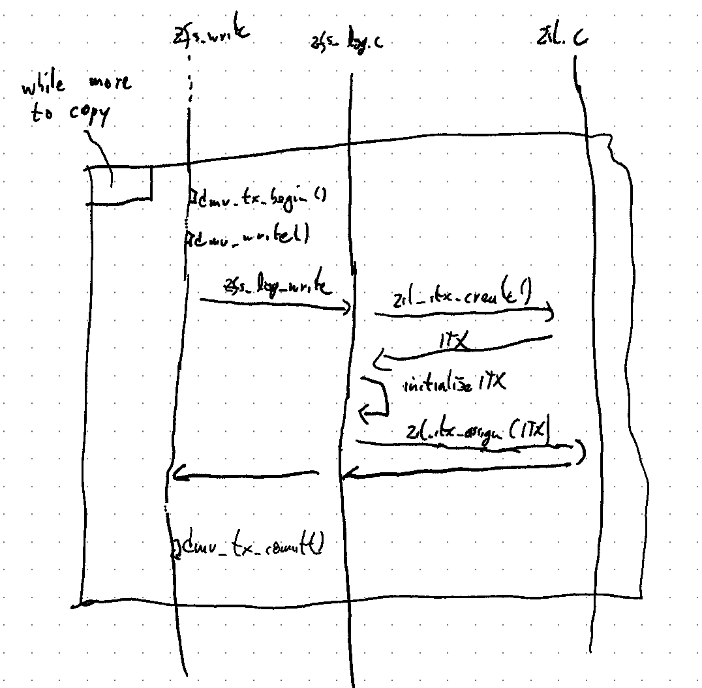
\includegraphics[height=8cm]{fig/zfs_log_write_sequence_diagram}
    \caption{Sequence diagram of the APIs involved in creating the ITXs for a \lstinline{write} system call.}
    \label{fig:zfs_log_write_sequence_diagram}
\end{figure}

\textbf{Alternative \#2}: Since we identified the ZIO pipeline as the most dominant contributor of latency in ZIL-LWB (Chapter~\ref{ch:lwb_analysis}), we considered to share LWBs as a concept between all ZIL kinds.
In that scenario, the ZIL kinds would merely be an alternative to the ZIO pipeline.
A prototype that bypasses ZIO but preserves the concept of LWBs has been presented at the OpenZFS 2020 Developer summit by \citeauthor{openzfsZILPerformanceImprovements2020}, targeting NVMe drives \cite{openzfsZILPerformanceImprovements2020}
We found this approach too restrictive for ZIL-PMEM:
\begin{enumerate}[noitemsep]
    \item The batching of many log records into fewer but larger LWBs adds unnecessary latency overhead.
        This notion is shared by the database community which has deemed such group commit schemes unfit for PMEM (see Section~\ref{sec:relwork:journalingandwals_adapted_to_pmem} on disk-oriented DBMSes).
    \item The design space for PRB/HDL would have been severely constrained.
        In particular, fully parallel logging to the same HDL would not have been possible because the LWB chain is inherently sequential.
        With our ITXG bypass for ZVOLs (see Section~\ref{sec:itxgbypass}), we want to explore whether parallel logging to PRB/HDL can increase the ZIL's scalability for a single dataset.
\end{enumerate}

\textbf{Conclusion}
Our design allows for sharing of ZFS's crash consistency guarantees towards userspace but leaves sufficient flexibility for each ZIL kind with regard to the persistent representation.
Our implementation shows little code duplication between ZIL-LWB and ZIL-PMEM, thereby hopefully keeping the maintenance burden low.
The state of each \lstinline{zilog_KIND_t} is truly private do the ZIL kind's implementation.
Neither ZIL-LWB nor ZIL-PMEM access the ITX-related state in the embedded \lstinline{zilog_t} directly, but only through the \lstinline{zilog_t} method that computes the commit list.
However, some design questions (see \ref{sec:zil_kinds:change} and \ref{sec:zil_kinds:suspend_resume}) as well as some LWB-specific APIs (see \ref{sec:zil_kinds:traversal} and \ref{sec:zil_kinds:callbacks}) remain.

\section{PMEM-aware SPA \& VDEV layer}\label{sec:pmemspavdev}
Prior to the work presented in this thesis, ZFS had no concept of persistent memory.
Fortunately, the requirements of ZIL-PMEM are very limited:
\begin{itemize}[noitemsep]
    \item \texttt{/dev/pmem} SLOGs must be recognized as such when they are added to the pool so that the ZIL-PMEM can be activated.
    \item The PMEM SLOG's allocatable space must be directly accessible via the PMEM programming model (load/store instructions, cache flushing, etc., see Section~\ref{sec:background:pmemprogrammingmodel}).
        If direct access is not possible, the PMEM SLOG VDEV must be considered faulty and pool import must be refused.
        We assume that direct access cannot be lost once it has been established.\todo{future work: memory hotplug}
\end{itemize}

We add a new boolean attribute \lstinline{is_dax} for \lstinline{disk} VDEVs in the zpool config format.
The attribute indicates whether the VDEV supports direct access through the Linux Kernel's DAX APIs.
DAX capability is determined by the \lstinline{zpool} command when creating or adding devices to a pool, using \lstinline{libblkid}.
When opening a VDEV marked \lstinline{is_dax}, the kernel module ensures that all of the block device's sectors are mappable as one contiguous range of kernel virtual address space.
Failure to establish this mapping fails the onlining process, leaving the VDEV in state \lstinline{VDEV_STATE_CANT_OPEN}.
By default, this state prevents the pool from being imported.
Note that the \lstinline{is_dax} feature applies to all VDEVs and is independent of ZIL-PMEM.
It merely records the fact that a VDEV is required to be directly accessible via the DAX APIs.
This ensures that future versions of ZFS can leverage DAX capability of main pool VDEVs without needing to change the on-disk format.
Consequently, \lstinline{is_dax} becomes an independent \textit{zpool feature}.

\section{The ZIL-PMEM ZIL Kind}\label{sec:zilpmemzilkind}
The changes described in the preceding sections prepare the way for the introduction of the new ZIL-PMEM ZIL kind.

\subsection{Activation}\label{sec:zilpmemzilkind:activation}
The ZIL-PMEM ZIL kind is used instead of ZIL-LWB based on the following rule:
\begin{displayquote}
  If the pool has exactly one SLOG and that SLOG is \lstinline{is_dax}, the ZIL kind is ZIL-PMEM. Otherwise, it is ZIL-LWB.
\end{displayquote}
This rule must be evaluated when the pool is imported or whenever the pool's SLOG VDEVs are about to change, i.e.,
during pool creation, on \lstinline{zpool add} and \lstinline{zpool remove}, and when \lstinline{zpool import} is told to drop log devices via the \lstinline{-m} flag.
To determine whether change ZIL kinds, we compare the resulting desired ZIL kind $k_{desired}$ with the \lstinline{zh_kind} value of any ZIL header in the pool.
If they do not match, we change the ZIL kind of all headers as described in Section~\ref{sec:zil_kinds:change}.
This implicit activation \& deactivation of ZIL kinds makes ZIL-PMEM completely transparent to the administrator, thereby fulfilling our requirement of simple administration.
ZIL-PMEM is automatically used if it supports the user-specified SLOG device configuration, i.e., a single /dev/pmem0 SLOG VDEV.
Otherwise, the system transparently falls back to ZIL-LWB.

\textbf{Note}: We have not yet implemented changing ZIL kinds after pool creation and thus not implemented the design described in the previous paragraph.
Instead, the \lstinline{zil_default_kind} kernel module parameter determines the ZIL kind of a newly created pool (ref. Section~\ref{sec:zil_kinds:change}).
If the ZIL kind is ZIL-PMEM, the implementation enforces that the pool config has exactly one SLOG VDEV that is \lstinline{is_dax}, and prevents any changes to the SLOG VDEV config.

\textbf{Alternative Design}
The implicit activation and deactivation based on the rule above makes the rule effectively part of the zpool's on-disk format because it must deliver deterministic results for an unchanged pool, regardless of any future software changes.
If the rule evaluation is not stable, the pool's ZIL kind could ``flap'' between imports which in turn would fail the import if there are unreplayed logs that prevent changing ZIL kinds.
It is worth reconsidering whether full implicitness is actually desirable or whether surfacing ZIL kinds to the administrator is acceptable.
For example, we could store the pool's \textit{current} ZIL kind in the MOS and provide an zpool command or property to change it.
Before the change is executed, the desired ZIL kind would check that the pool configuration is supported and fail the change operation if that is not the case.
In the case of ZIL-PMEM, this hook would evaluate the rule above.
Any changes to the zpool topology (\lstinline{zpool add}, \lstinline{remove}, \lstinline{import} with \lstinline{-m}), would also invoke this hook.
% Implicit activation and deactivation could still be achieved by moving the rule evaluation to the \lstinline{zpool} command.

\subsection{PMEM Space Reservation \& PRB Construction}\label{sec:zilpmemzilkind:spacereservation}

If the pool's ZIL kind is ZIL-PMEM, we reserve all of the allocatable space on the PMEM SLOG VDEV for PRB.
To accomplish this, we introduce a new allocation class called \lstinline{exempt} that is, by convention, never used for SPA allocations.
In our current implementation, the \lstinline{zpool} command assigns this allocation class automatically to \lstinline{is_dax} SLOG VDEVs, instead of the \lstinline{log} allocation class.
Note that the VDEV labels, which attribute the VDEV to the zpool and store parts of the zpool config, are located outside the allocatable space.
Readers and updaters of VDEV labels continue to use block device IO (\lstinline{zio_read_phys} and \lstinline{zio_write_phys}).

ZIL-PMEM uses \lstinline{dax_direct_access} API (ref. Section~\ref{sec:background:pmemconfiguration}) to discover the memory mapping of the \lstinline{exempt} SLOG VDEV's allocatable space and constructs the pool's PRB instance on top of it.
\begin{enumerate}
\item The pool import procedure allocates the \lstinline{prb_t} and stores the pointer in the DRAM object that represents the imported pool (\lstinline{spa_t}).
When the pool is exported, the \lstinline{spa_unload} procedure frees the \lstinline{prb_t}.
The \lstinline{prb_t}'s lifetime is thus a contiguous sub-span of the lifetime of \lstinline{spa_t}.
\item  Immediately after allocating the PRB, pool import sets up the chunk objects and adds them to the PRB.
If the pool is being created, we reset the chunks to a known PMEM state (\lstinline{prb_chunk_initialize_pmem}) before adding them to PRB.\todo{impl is a little different, doesn't matter?}
\end{enumerate}

We use a simplistic partitioning scheme to divide the PMEM space into chunks.
The main advantage of the scheme is that it does not need to persist any metadata:
\begin{itemize}[noitemsep]
    \item Chunks have a hard-coded size of 128~MiB.
    \item We partition the PMEM SLOG VDEV's allocatable space as a contiguous array of 128~MiB segments, starting at offset zero.
    \item Assuming $A$~bytes of space, this yields \lstinline{nchunks := A>>27} chunks and less than 128~MiB of wasted space at the end of the allocated space.
    \item We do not store \lstinline{nchunks} anywhere. Instead, we prohibit online resizing of the PMEM SLOG VDEV which allows us to deterministically re-compute the value.
\end{itemize}

\textbf{Note:} Over the course of implementing and testing ZIL-PMEM, we observed that instead of attempting to exempt the PMEM SLOG VDEV's space from regular allocation, it is probably preferable to pre-allocate all the PMEM space on the SLOG VDEV from the SPA.
The reason is that some lesser-known components of ZFS expect that unallcoated SPA space can be overwritten in the background (e.g., the code that supports TRIM or the \textit{VDEV initialize} functionality).
Also, there is existing infrastructure to prevent removal of SLOGs with existing SPA allocations, for which we currently require a ZIL-PMEM specific special case.

\subsection{Dataset \& HDL Lifecycle Synchronization}\label{sec:zilpmem:hdllifecycle}
Whereas \lstinline{prb_t} and \lstinline{spa_t}'s allocation lifecycles line up well, the same is not true for datasets and HDLs:
HDLs must be set up during pool import and must not be torn down via \lstinline{prb_teardown_hdl} until either their dataset destroyed or the zpool is exported.
In contrast, the per-dataset runtime state (\lstinline{dsl_dataset_t}, its \lstinline{objset_t} and the objset's \lstinline{zilog_t}) is allocated ``on demand'' when its consumer, the ZPL code, \textit{holds} it by its object ID in the MOS.
Specifically, the first holder performs the allocation and recovers state from the corresponding persistent structure (\lstinline{dsl_dataset_phys_t}, \lstinline{objset_phys_t} and, partially, \lstinline{zil_header_t}).
Conversely, if there was already another holder, the existing DRAM object is shared.
Once a consumer no longer needs to hold a dataset, it \textit{releases} its hold on the instance.
The last consumer that releases the structure frees the DRAM object.
(Holds and releases are implemented through reference counting.)

The mismatch of HDL and dataset object lifetimes is relevant for ZIL-PMEM because the state in HDL, in particular the holds on chunks established during claiming, outlives the instantiation(s) of \lstinline{zilog_pmem_t}.
Our solution is to add a search tree to \lstinline{spa_t} which we call \textit{HDL map}.
It maps from the dataset's object set ID to its HDL.
We add the necessary callbacks to synchronize the \textit{HDL map} with the dataset layer.
%git show ':/make it work (high-level description of what we do in commit msg)'
\begin{itemize}[noitemsep]
    \item During pool import, after setting up the PRB but before claiming, we iterate over the head datasets%
        \footnote{Head datasets are ZPL filesystems, ZVOLs, and clones thereof. ``Behind'' a head dataset can be one or more snapshots.}
        in the pool, set up the HDLs for each of them, and add them to the \textit{HDL map}.
    \item When a new head dataset is created (\lstinline{dmu_objset_create_impl_dnstats} and \lstinline{dmu_objset_clone_sync}), we set up its HDL and add it to \textit{HDL map}.
    \item When a head dataset is destroyed (\lstinline{zil_destroy_sync}), we tear down the HDL and remove it from the \textit{HDL map}.
\end{itemize}

Whenever the ZIL-PMEM implementation needs access to the HDL, it looks up the HDL in the \textit{HDL map} and acquires a reference to it.
We use reference counting to assert that there are no dangling references when the head dataset is destroyed and the HDL is torn down.
We protect the \textit{HDL map} against concurrent modifications using ZFS's \textit{read mostly lock} which is a reader-writer-lock that is optimized for reads.
Figure~\ref{fig:zilpmem:datasethdlsync} visualizes the constellation of objects, their lifetimes, and reference relationships.

\begin{figure}[H]
    \centering
    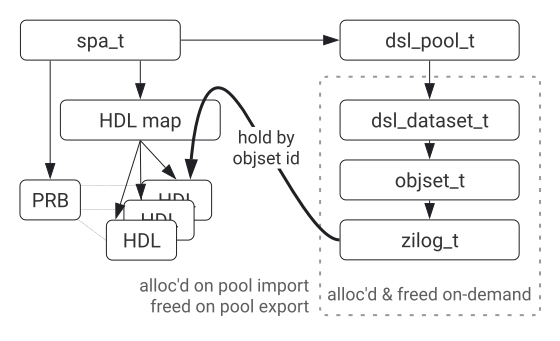
\includegraphics{fig/zilpmem_dataset_hdl_sync}
    \caption{The different allocation lifecycles of HDLs and datasets, and how we bridge them for ZIL-PMEM.}
    \label{fig:zilpmem:datasethdlsync}
\end{figure}

\subsection{ZILOG\_PMEM\_T}\label{sec:zilpmem:zilog}
The \lstinline{zilog_pmem_t} structure and its methods in the \lstinline{zilpmem_vtable} implement the ZIL-PMEM ZIL kind.
Its role is that of an adaptor between the shared high-level ZIL code (\textit{itxg} structure) and the dataset's HDL that is associated with the dataset via the \textit{HDL map}.
Apart from the exceptions listed below, the methods in the vtable are thin wrappers around HDL's interfaces.
The general pattern for a ZIL-PMEM method is as follows:
\begin{enumerate}[noitemsep]
    \item Acquire a reference to the dataset's HDL from \textit{HDL map}.
    \item Invoke the HDL method.
    \item Release the HDL reference.
\end{enumerate}
To avoid reference counting overhead for HDLs on the write path, we acquire a HDL reference once when the ZIL is opened during mounting and hold it in the \lstinline{zilog_pmem_t} until the dataset is unmounted.

The following cases required additional code to adapt between the two domains:
\begin{description}
    \item[Error Handling During Pool Import \& Claiming]
        ZIL kinds inherit the behavior of ZIL-LWB for integrity checking and claiming of the ZIL during pool import.
        ZIL-LWB checks the LWB chain twice.
        The first pass (\lstinline{zil_check_log_chain}) checks for log corruption so that it can fail the pool import early if the log is corrupt.
        The second pass (\lstinline{zil_claim}) does ZIL-LWB's equivalent of claiming and stores the maximum claimed log record number in the ZIL header.
        It discards traversal errors because it assumes that no online log corruption happend since the first pass.
        (Note that \lstinline{zil_claim} does have a return value, but only due to software-technical reasons. It must always return zero.)
        ZIL-LWB's approach opens a window for time-of-check vs time-of-use bugs which we discovered and reported during development \cite{OpenZFSGithubIssueHandlingOfLostClaimedNotReplayedLogRecords}.
        In contrast, PRB/HDL does checking and claiming in a single pass (\lstinline{prb_claim}), reports corrupted log state through its return value, and is designed to correctly handle online log corruption during claiming and replay (see Section~\ref{di:prb:ccrecovery}).

        Due to time constraints, we have not refactored the zpool import procedure to allow claiming to fail.
        Until that shortcoming of our implementation is addressed, we trigger a kernel panic if \lstinline{prb_claim} returns an error.

    \item[ZIL Header Updates]
        Remember from Section~\ref{di:prb:api:hdl} on the PRB/HDL API that the responsibility of \textit{persisting} the ZIL-PMEM header is split:
        HDL APIs that update the ZIL header return the updated version through an \textit{out}-parameter and the API consumer is responsible for persisting the update to the main pool.

        Unlike DMU consumers, the ZIL implementation itself is responsible for queuing up changes that need to applied for the \textit{open}, \textit{quiescing} and \textit{syncing} txg.
        When \textit{txg sync} is syncing the \lstinline{syncing_txg}, it invokes the \lstinline{zil_sync} API of each \lstinline{zilog_t}.
        The role of \lstinline{zil_sync} is to set the ZIL header buffer that is stored in \lstinline{objset_phys_t::os_zil_header} to the state that shall be persisted in the \lstinline{syncing_txg}.
        \textit{Txg sync} then uses this buffer's content when it writes out \lstinline{objset_phys_t} to the on-disk tree structure.

        ZIL-PMEM queues the updated header values returned by the HDL APIs in a 4-ary array that is indexed by \lstinline{[txg&3]}.
        Each cell contains the tuple \lstinline{(txg: u64, header: zil_header_pmem_t)}.
        A header update \lstinline{(txg_u, header_u)} overwrites the cell at index \lstinline{txg_u&3}.
        Updates must only be made from the \textit{open} or \textit{quiescing} txgs.
        \lstinline{zilpmem_sync} then reads then cell \lstinline{C} at index \lstinline{updates[syncing_txg&3]}.
        If \lstinline{C.txg == syncing_txg}, it stores \lstinline{C.header} in the \lstinline{objset_phys_t::os_zil_header} field to be picked up by \textit{txg sync}.
        Otherwise, it leaves \lstinline{objset_phys_t::os_zil_header} unmodified.

    \item[zil\_commit]
        We implement \lstinline{zil_commit} as follows:
        \begin{enumerate}[noitemsep]
            \item Acquire a \lstinline{zilog_pmem_t}-wide mutex.
            \item Get the \textit{commit list} from the \textit{itxg} data structure.
            \item Write each ITX (i.e., log record) on the commit list to the HDL using \lstinline{prb_write_entry}.
                A new generation is started for every ITX to encode the sequential log structure.
            \item Release the mutex.
        \end{enumerate}
        The mutex ensures that \textbf{committers are serialized}.
        This is critical for the correctness of \textit{sync} or \textit{fsync} which are cummulative.
        Assume two threads $A, B$ that issue the \textit{sync} system call.
        Assume $A$ starts a \textit{sync} system call and drains all ITXs from the \textit{itxg} into its commit list.
        If $A$ is now preempted by $B$ which also starts a \textit{sync} system call, $B$'s commit list will be empty.
        $B$ would return to userspace, giving the caller the impression that all dirty data has been synced, although they still need to be written to the HDL by~$A$.
        $B$ must therefore wait for $A$ before returning to userspace.

        Starting a new generation for every entry ensures that the commit list's entries will be replayed in commit list order.
        The \lstinline{zilog_pmem_t}-wide mutex already serializes the start of the new generations as required by the HDL API, see Section~\ref{di:prb:api:write}.

        Serializing the entire \lstinline{zil_commit} call allows for less parallelism than ZIL-LWB's \textit{commit ITXs}.
        Commit ITXs implement a sort of pipelining by allowing log writers to issue LWB ZIOs in parallel while ensuring that they only return from \lstinline{zil_commit} after all LWBs up to and including the log writer's last LWB have been written.
        Whereas a similar approach could be applied to ZIL-PMEM in principle by mapping parallel writers to the same generation, the current implementation of commit ITXs is too tightly coupled to the concept of LWBs and the ZIO pipeline.

    \item[WR\_NEED\_COPY Chunking]
        Remember from Section~\ref{openzfs:the_zil_api} that the ZIL allocates ITXs for \textit{all} changes to a dataset in DRAM.
        The ITXs are queued in the \textit{itxg} structure from where they are either \lstinline{zil_commit}ted or freed when the txg syncs.
        To avoid unnecessary memory usage and performance overhead, ITXs that log large \textit{write} operations do not always contain a copy of the written data.
        Instead, the ITX is marked as a \lstinline{WR_NEED_COPY} ITX.
        Such ITXs only contain the object number of the DMU object and the byte range within the object that was written.
        The creation of the log record is deferred until \lstinline{zil_commit} which creates the actual \textit{write} records whose payload data is read back in from the DMU object.

        To support WR\_NEDD\_COPY in ZIL-PMEM, we implement an isolated structure that turns a single \lstinline{WR_NEED_COPY} record into an iterator over \textit{write} log entries.
        \lstinline{zil_commit} writes each entry yielded by the iterator to the HDL using \lstinline{prb_write_entry}.
        Whereas the repeated chunk acquisition and dependency tracking during each HDL write incurs a small overhead, it also increases fairness among HDLs if the commit slots are contended.

\end{description}

\subsection{ITXG Bypass For ZVOL}\label{sec:itxgbypass}
ZIL kinds are forced into the \textit{commit list} model that defined by the \textit{itxg} structure which is shared among all ZIL kinds.
This model leads to an inherently sequential representation of the ZIL contents:
ZIL-LWB is a long chain of log entries grouped in LWBs, and ZIL-PMEM starts a new generation for every entry on the commit list to encode it properly.
We believe that this architecture is the best compromise for consistent behavior across ZIL kinds, performance, code duplication, and maintainability.
(See Section~\ref{sec:zil_kinds:alternatives} for a reflection on alternatives.)
Our evaluation in the next chapter shows that ZIL-PMEM yields significant latency benefits and comes close to saturating PMEM bandwidth when performing synchronous IO from four threads to \textit{separate} datasets.
However, we also wanted to explore the performance potential of PRB/HDL without the limitations of \textit{itxg} but the same log record types and guarantees towards upper layers.
The result is an \textit{ITXG bypass} mode for ZIL-PMEM which we present in this subsection.

\subsubsection{ZVOLs And The ZIL}\label{sec:itxgbypass:openzfsbackground_zvols}
The mode only works for ZVOLs which are sparsely allocated virtual block devices.
Other block device consumers, e.g., virtual machines or other file systems, can treat the ZVOL as any other block device exposed by the kernel.
ZVOLs are implemented as a dataset with a single DMU object that contains the virtual block device's data.
When a block device driver accesses the ZVOL block device (\textit{read, write, discard}), ZFS maps the block device operations to DMU operations on the object.
The modifications are logged to the ZIL as \textit{write} and \textit{truncate} ITXs.
If the block device operation has synchronous semantics, ZFS calls \lstinline{zil_commit} before acknowledging completion of the block device operation.
The following pseudo-code describes how the ZVOL processes a block device operation.

\begin{lstlisting}[style=figurepseudocode]
Input:
    op      block device operation
    zv      zvol
Steps:

    if op.pre_flush:
        zil_commit(zv.dmu_object_id)

    match op {
        Read(...) => {
            dmu_read(zv.dmu_object, op.buf, ...)
        },
        Write(...) => {
            tx := dmu_transaction()
            dmu_write(tx, zv.dmu_object_id, ...)
            itx := zil_itx_create(...)
            zil_itx_assign(itx)
            dmu_tx_commit(tx)
        },
        Discard(...) => {
            // analogous
        }
    }

    if op.post_flush:
        zil_commit(zv.dmu_object_id)

    op.done() // acknowledge completion

\end{lstlisting}

The Linux kernel's model for block-level IO is based on the assumption that storage devices are asynchronous.
IO operations are represented by a \lstinline[style=figurepseudocode]{struct bio} that is eventually submitted to the IO stack (\lstinline{submit_bio}), potentially scheduled or merged, and then passed down to the block device driver which issues operations to the hardware.
Eventually, the hardware reports completion to the driver and the driver marks the IO as completed (\lstinline{BIO_END_BIO}).

By default, ZVOLs uses a thread pool (\textit{taskq}s) to process outstanding block device IO asynchronously and in parallel.
The \lstinline{zvol_request_sync=1} tunable changes this behavior to synchronous mode where the procedure outlined above is executed in synchronously in \lstinline{submit_bio}.
We will refer to this tunable in the Section~\ref{sec:eval:zvols_ad_itxg_bypass} of the evaluation.

\subsubsection{ITXG Bypass}

We observe that the ZIL's fully sequential structure is unnecessary for ZVOLs because block device consumers must already account for device-internal caching.
If a block device consumer actually requires consistency at a given point in time, it already \underline{\smash{explicitly}} indicates this to the block layer.
In Linux, this indication is either given by the \lstinline{bio} operation's type (\lstinline{REQ_OP_FLUSH}) or the pre-flush or post-flush flags (\lstinline{REQ_PREFLUSH}, \lstinline{REQ_FLUSH}).

We leverage this observation as follows.
We do not queue ITXs in \textit{itxg} but write all log entries directly to the HDL from within the DMU transaction.
By default, we do not start a new generation, thereby enabling parallel writes to the HDL.
If the block device consumer requests a flush, we serialize HDL access to start a new generation.%
\footnote{Remember that external synchronization on generation start is a requirement of PRB/HDL, see Sections~\ref{di:prb:write:hdlscoped} and \ref{di:prb:api:write}.}
We use a reader-writer-lock to achieve this behavior, as illustrated by the following pseudo-code.

\begin{lstlisting}[style=figurepseudocode]
Input:
    op      block device operation
    zv      zvol
      rwl        reader-writer-lock
      start_gen
Steps:
    if op.pre_flush || op.post_flush:
        zv.rwl.write_lock()
        zv.start_gen = true
    else:
        zv.rwl.read_lock()
        if zv.start_gen:
            zv.rwl.upgrade()

    match op {
        Read(...) => { ... }
        Write(...) => {
            tx := dmu_transaction()
            dmu_write(tx, zv.dmu_object_id, ...)
            itx := zil_itx_create(...)
            prb_write_entry(
                itx.into_log_entry(),
                needs_new_gen=zv.start_gen
            );
            assert zv.start_gen => zv.rwl.holding_write_lock
            if zv.start_gen:
                zv.start_gen = false
            dmu_tx_commit(tx)
        },
        Discard(...) => { /* analogous */ }
    }

    if op.post_flush:
        assert zv.rwl.holding_write_lock
        zv.start_gen = true

    op.done() // acknowledge completion
\end{lstlisting}

The following Figure~\ref{fig:itxg_bypass_viz} provides an example sequence of two threads that issue block IO operations to the same ZVOL in parallel.

\begin{figure}
    \centering
    \includegraphics{fig/itxg_bypass_viz.pdf}
    \caption{Example timeline for the IO operations of two threads that write to the same ZVOL, with the ITXG bypass mode enabled.
        The first write operation after a flush detects that \lstinline{zv.start_gen} is set and hence upgrades its read-lock to a writer-lock so that it can write the first entry of the new generation sequentially.
        As soon as it is done, it sets \lstinline{zv.start_gen = false} and relinquishes the writer lock.
        Subsequent writes until the next flush operation acquire a read lock, observe \lstinline{zv.start_gen  = false}, and write to HDL in parallel which results in multiple entries for generation 43.
        Entry F, which is the first entry after the second flush, starts a new generation.
    }
    \label{fig:itxg_bypass_viz}
\end{figure}


\chapter{Evaluation}\label{ch:eval}
In this chapter we evaluate whether ZIL-PMEM meets the project goals established in Section~\ref{sec:requirements}.

\section{Usability \& Architecture}

Our high-level requirements for ZIL-PMEM were: simple administration, sharing of PMEM as a pool-wide resource, coexistence with the existing ZIL(-LWB), and conservation of the same crash consistency guarantees towards userspace.
\begin{description}[noitemsep]
    \item[Simple Administration] We have proposed a design where ZIL-PMEM is automatically activated if exactly one PMEM SLOG VDEV is configured (Section~\ref{sec:zilpmemzilkind:activation}).
        This would make ZIL-PMEM completely transparent to the administrator and not bring any user-visible change in ZFS's administrative tools.
        However, our implementation does not yet support changing the ZIL kind of a zpool after its creation (Section~\ref{sec:zil_kinds:change}).
    \item[Pooled Storage] PRB wraps the PMEM SLOG device and shares it as a pool-wide resource among all HDLs / datasets.
    \item[Coexistence] The introduction of \textit{ZIL Kinds} allows for coexistence of ZIL-LWB and ZIL-PMEM in code and at runtime.
        The layer at which ZIL kinds were introduced in the architecture allows for sharing of all code that deals with the ZIL's logical structure but enables coexistence of different persistence strategies.
    \item[Same Guarantees] ZIL-PMEM maintains the same crash consistency guarantees as ZIL-LWB towards userspace, courtesy of the shared logical structure and PRB/HDL's guarantees.
\end{description}

\section{Correctness}

We use unit tests and integration tests to validate our implementation.

\subsection{Testing Strategy for PRB/HDL}\label{sec:eval:correctness:prb}

We are able to test PRB/HDL in userspace since it is part of \textit{libzpool}.
\textit{libzpool} is a shared library that contains the majority of ZFS's kernel code, compiled for userspace.
It is used by \textit{zdb} (the ZFS debugger) and the \textit{ztest} stress testing tool.
We implement our unit tests in Rust to leverage its expressive type and macro system, rich standard library, and built-in testing harness.
We use the popular \textit{bindgen} crate to generate the bindings to \textit{libzpool} and implement a small set of idiomatic wrappers around PRB/HDL to reduce boilerplate code in our tests.

\subsubsection{API Walkthrough}
We codify the walkthrough of the PRB/HDL API that we presented in Section~\ref{di:prb:api} in a large test:
\begin{enumerate}[noitemsep]
    \item Allocate a ZIL header on the stack.
    \item Create a chunk whose space is allocated from the heap.
    \item Construct PRB and add the chunk to it.
    \item Setup a HDL.
    \item Create a log for the HDL.
    \item Write two entries for $txg=2$ with body values $23$ and $42$ to the HDL.
    \item Teardown the object set.
    \item Destroy the PRB with \lstinline{free_chunks=false}. This moves ownership of the chunk moves back from PRB to us.
    \item Construct a new PRB instance with the same chunk.
    \item Setup a HDL from the ZIL header.
    \item Trigger claiming.
    \item Trigger replay, and record the replay callback invocations.
        For each invocation, we read the body length and content, and assert that no read error occurred.
        We record body content and the ZIL header update as records in a list.
        We report successful replay for every callback invocation.
    \item After replay is complete, we compare the recorded list's contents to the expected replay order.
\end{enumerate}

\subsubsection{Correct Handling Of Obsolete Entries}
PRB/HDL assumes that there are only three unsynced txgs at any given time.
This manifests in frequent use of the \lstinline{txg&3} indexing idiom that is common in ZFS.
Whenever state needs to be kept for each of the unsynced txgs, a 4-ary array is used to represent it.
The \lstinline{txg&3}'th element in the array then contains the state for \lstinline{txg}.
The value of \lstinline{txg} is repeated within the per-txg state to detect when an array element is re-used.

With regard to PRB, an entry $E_i$ must only be written to PMEM if its txg $E_i.txg$ is newer than the HDL's highest-ever written txg $T_{max}$, or if it is one of $T_{max}$, $T_{max}-1$, or $T_{max}-2$.
The reason is the fixed number of three counters in the entry header that are used for dependency tracking (ref. Section~\ref{di:prb:deptrack}).
We add tests that ensure that the \lstinline{prb_write_entry} API returns an error if entries are written that do not meet this criterion.
We also test the behavior of replay to ensure that, if the write path implementation were incorrect, replay would identify the problem with a distinct error code.

\subsubsection{Replay Algorithm}
We structure the PRB/HDL implementation such that it becomes possible to test the core replay logic that we described in Sections~\ref{di:prb:replayapproach},~\ref{di:prb:deptrack},~\ref{di:prb:modeldatacorruption} and ~\ref{di:prb:ccrecovery}:
The idea is to isolate the core logic in a function \lstinline{replay_resume} that takes the following arguments as input:
\begin{description}[noitemsep,leftmargin=1.5cm,labelindent=1cm]
    \item[NodeSet] The set of entries, represented as \textit{replay nodes}, that were discovered for the HDL.
    \item[ReplayState] A pointer to the DRAM representation of replay state,
    \item[Callback] A callback that receives as arguments
    a) the replay node and b) a pointer to the replay state that needs to be persisted to the ZIL header during replay.
\end{description}
\lstinline{replay_resume} constructs the replay sequence from \textit{NodeSet} and then invokes the \textit{Callback} for each entry that needs to be replayed.
The \lstinline{prb_claim} API uses \lstinline{replay_resume} for ZIL headers in state \textit{logging} to determine $E_{seal}$, and for a dry-run of replay for headers in state \textit{replaying} to detect missing entries early during pool import (see Section~\ref{di:prb:ccrecovery}, Step~\ref{ccReplay:claimscan}).
It provides its own \textit{Callback} (\lstinline{prb_claim_cb}) which checks that all replay nodes' bodies can be read without error, using the \lstinline{prb_replay_read_replay_node} API that the actual replay callback is going to use as well.
The \lstinline{prb_replay} API uses \lstinline{replay_resume} for actual replay.
Its \textit{Callback} (\lstinline{prb_replay_cb}) serializes \textit{ReplayState} to the representation stored in the ZIL header, builds the ZIL header update, and invokes the user-provided replay callback.
Figure~\ref{fig:eval:prb_replay_resume_architecture} visualizes this architecture.

\begin{figure}[H]
    \centering
    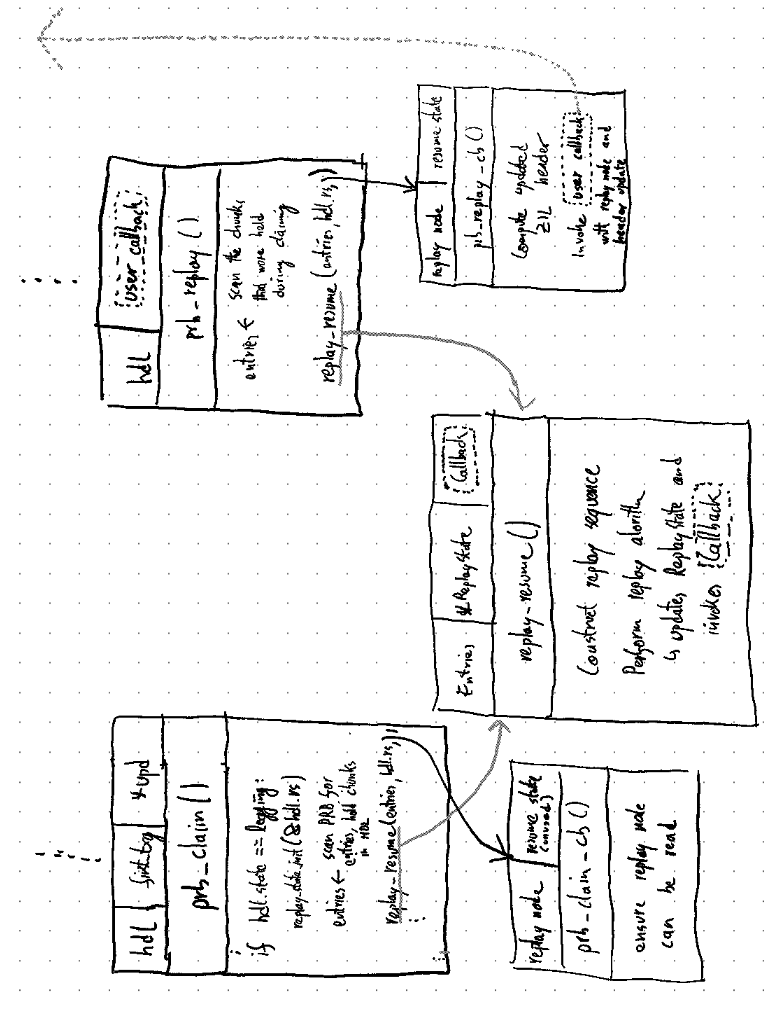
\includegraphics{fig/prb_replay_resume_architecture}
    \caption{The architecture that enables code re-use and testability for the core replay logic.}
    \label{fig:eval:prb_replay_resume_architecture}
\end{figure}

This factorization of responsibilities provides maximum flexibility for testing because it decouples the storage substrate (PRB \& chunks) from the per-HDL logical log structure:
\begin{description}[noitemsep,leftmargin=1.5cm,labelindent=1cm]
    \item[Independence of PRB \& Chunks]
        It is not necessary for testing code to mock PRB or chunks.
        It is not even necessary to create mock log entries.
        Instead, it is sufficient to allocate arbitrary \textit{replay node} structures and to put them into the \textit{EntrySet}.

    \item[Independence of ZIL-PMEM]
        The integration logic in ZIL-PMEM is not involved in testing PRB/HDL.
        This means that PRB/HDL's replays behavior can be validated in isolation.
        It also simplifies the testing code because there no need to mock the environment that ZIL-PMEM expects, e.g. SPA, DMU, and VDEVs.

    \item[Crash Consistency Testing]
        To test crash consistency and correctness for resumed replay, the testing code can simply forge an arbitrary replay state in DRAM and invoke \lstinline{replay_resume} with it.
\end{description}

We leverage Rust's macro system to define test cases in a concise and expressive manner.
Our goal is to minimize the mental step from the two-dimensional grid visualization to a test case (example: Figure~\ref{fig:prb_hdl_log_structure_example} in Section~\ref{di:prb:logstructure}).
The following code snippet is an excerpt from the test suite:

\begin{lstlisting}[style=figurepseudocode]
TestSet {
  title: "I- shape",
  entries: maplit::btreemap! {
    // SynthEntry(txg,gen,gsid, (<counters>))
    "A" => SynthEntry(3,10,1, ([(0,0),(0,0),(0,0)])),
    "B" => SynthEntry(4,10,2, ([(0,0),(0,0),(0,0)])),
    "C" => SynthEntry(5,10,3, ([(0,0),(0,0),(0,0)])),
    "D" => SynthEntry(4,11,1, ([(5,1),(4,1),(3,1)]))
  },
  tests: vec![
    test! {
      "tail truncation ok",
      claim_txg = 1,
      // hide entry D during replay and assert that
      // replay does not complain
      stages = stages!(single, hide=&["D"], check=OK,),
      // expected replay callback invocations
      expect_replay = vec!["A", "B", "C"],
    },
    test! {
      "'A missing' detected, but rest of gen is replayed",
      claim_txg = 1,
      // hide entry A during replay and ensure that replay
      // complains about missing entries
      stages = stages!(single, hide=&["A"], check=M_ENTRIES,),
      // expected replay callback invocations
      expect_replay = vec!["B", "C"],
    },
  ],
}
\end{lstlisting}

Our tests check the following properties of the replay code:
\begin{description}[noitemsep,leftmargin=1.5cm,labelindent=1cm]
    \begin{minipage}{0.59\textwidth}
    \item[Shapes]
            We test replay for different ``shapes'' in the 2-D grid.
            For example, an ``I-'' as described the snippet above and depicted to the right.
        \end{minipage}
        \begin{minipage}[c]{0.3\textwidth}
            \includegraphics[trim=0cm 0.42cm 0cm 0.42cm,clip]{fig/correctness_eval_example_I-_shape.pdf}
        \end{minipage}
    \item[Claim Txg] We ensure that log entries for txgs $\le precrash\_txg$ are not replayed because their effect is already part of the dataset's state.
        In the code base, it is more common to refer to $claim\_txg = precrash\_txg + 1$.
    \item[Missing Entry Handling] We test the handling of missing entries in both the already replayed and the still-to-be-replayed parts of the replay sequence, as well as the special cases for missing entries in the last generation.
    \item[Resumability] We test resumability of \lstinline{replay_resume} for the cases of missing entries, re-appearing entries, and no change of \textit{EntrySet} between resume attempts.
    \item[Entry Reappearance] We validate that re-appearing entries that are ordered \textit{before} the last-replayed entry are ignored, and that re-appearing entries in the \textit{unreplayed} part are discovered and replayed.
\end{description}

\subsubsection{Testing Runtime Assertions}
We make heavy use of runtime assertions to protect against existing and future implementation errors.
On the recovery path, which is not performance-critical, assertions are enabled in release builds.
On the write path, most assertions are only enabled for debug builds.
In \textit{libzpool}, which is used by our userspace tests, assertions are always enabled.

We modify \textit{libzpool} such that our test suite can install a callback that is invoked when a runtime assertion fails.
The callback receives the formatted panic message as an argument.
We use this mechanism to implement \textit{crash tests} which assert that a piece of test code triggers a runtime assertion.
The panic message is used to identify the assertion since cross-FFI stack unwinding is not yet supported in Rust.

At this time, we use crash tests to ensure that incorrect usage of the PRB API is detected at runtime:
\begin{itemize}[noitemsep]
    \item Operations on a HDL in the wrong state, e.g., replay of a HDL which was not claimed.
    \item Attempts to set up a HDL that has already been set up.
    \item Writes that exceed the maximum allowed chunk size.
    \item Correct interplay of garbage collection and PRB during PRB allocation (critical for pool export).
\end{itemize}

\subsection{Testing Strategy for ZIL-PMEM}\label{sec:eval:correctness:zilpmem}

Our changes to ZFS have less coverage than PRB/HDL.
The OpenZFS project has the following existing facilities for testing:
\begin{description}[noitemsep]
    \item[ZFS Test Suite (ZTS)] The ZFS Test Suite is a set of automated integration tests that assert behavior of the kernel module and CLI tools.
        ZTS is implemented in shell and provides a significant amount of functional tests that exercise both the data path and administrative layer of ZFS.
    \item[ztest] The \textit{ztest} tool is a user-space binary that links against \textit{libzpool} and stress-tests core components of ZFS that are shared among all supported platforms.
        It define routines that imitate the kernel module's use the core components' APIs.
        The stress-testing aspect comes from repeatedly dispatching these routines to a pool of threads.
        Additionally, IO failures are injected through ZFS's fault injection facilities (ref. Section~\ref{sec:rel_work:fault_injection}), and system crashes are simulated by randomly killing the \textit{ztest} process.
        \textit{ztest} is particularly useful for exposing race conditions in the administrative layer that would not be discovered by the mostly sequential usage in the ZTS.
\end{description}

We identify three major challenges in adapting OpenZFS's testing infrastructure to ZIL-PMEM:
\begin{description}[noitemsep]
    \item[Dimensionality] ZIL kinds add a new dimension in the configuration space that has not been anticipated by the designers of ZTS and ztest.
        Since all ZIL kinds should be functionally equivalent, the ideal testing strategy would execute all existing tests for each ZIL kind.
        However, the testing harnesses for ZTS does not have the infrastructure for this task.

    \item[File VDEVs] Both ZTS and ztest rely heavily on the \textit{file} VDEV type.
        \textit{File} VDEVs are plain files that can be used in lieu of block devices when constructing a zpool.
        They are problematic for ZIL-PMEM because we only added support for DAX block devices, not files.
        To support \textit{file} VDEVs for ZIL-PMEM, the ZFS kernel module would need to \lstinline{mmap} the file in the kernel.
        We are unaware of a kernel API that allows an external module, such as ZFS, to accomplish this.
        For correctness, the memory mapping would further need to map directly to PMEM, i.e., be located on a Linux filesystem mounted with the \textit{dax} mount option (cf. Section~\ref{sec:background:pmemconfiguration}).

    \item[VDEV Management]
        A significant number of tests in ZTS and ztest address the different ways to change the pool's VDEV config, e.g., addition, removal, growing, and offlining of VDEVs.
        This is related to ZIL-PMEM because our design goal is to transparently switch ZIL kinds based on the absence or presence of exactly one PMEM SLOG VDEV.
        However, the current state of our implementation does not yet support changing ZIL kinds after pool creation and prevents changes to the SLOG VDEV config to ensure that the PMEM SLOG VDEV is always present (Section~\ref{sec:zil_kinds:change}).
        Thus, many tests that should work correctly in the final implementation currently fail when attempting to change the VDEV config.
\end{description}

We modify \textit{ztest} as follows:
\begin{description}[noitemsep]
    \item[Mocking]  \textit{Ztest} mocks the representation of datasets (\lstinline{ztest_ds_t}) but uses the production implementation of the \lstinline{objset_t} and \lstinline{zilog_t} types and related APIs.
        Since ZIL kinds do not change the public ZIL API significantly, the parts of ztest that are concerned with mocking the dataset lifecycle, such as dataset creation, snapshotting, destruction, and cloning, only required minor modifications.
    \item[ZIL-LWB Specific Assertions] Some of the \textit{ztest} routines assert ZIL-LWB specific state.
        We make these assertions conditional, based on the active ZIL kind.
        If the ZIL kind is ZIL-LWB, we downcast \lstinline{zilog_t} to \lstinline{zilog_lwb_t} to perform the check.
    \item[Configurable ZIL Kinds] We add a command line switch to \textit{ztest} to configure the default ZIL kind that is used for the test pool.
        This is equivalent to the \lstinline{zil_default_kind} kernel module parameter (Section~\ref{sec:zil_kinds:change}).
    \item[VDEV Management] There are several \textit{ztest} routines that randomly add and remove VDEVs, inlcuding SLOG devices.
        We change the function that selects the target VDEV such that it never returns a SLOG device if the pool's ZIL kind is ZIL-PMEM.
\end{description}
We have not added any ZIL-PMEM specific assertions or additional test routines to \textit{ztest}.
To get coverage for ZIL-PMEM and ZIL-LWB, it is necessary to run ztest twice with the respective values for the command line flag.
% Future work should extend the \textit{zloop.sh} script which already provides infrastructure to run \textit{ztest} with different combinations of parameters (i.e., CLI flags).

Regarding the ZTS, the following tests are relevant for the ZIL:
\begin{lstlisting}[style=figurepseudocode]
$ fdfind --print0 slog ./tests | xargs -0 grep log_assert | ...
slog_001_pos.ksh  Creating a pool with a log device succeeds
slog_002_pos.ksh  Adding a log device to normal pool works
slog_003_pos.ksh  Adding an extra log device works
slog_004_pos.ksh  Attaching a log device passes
slog_005_pos.ksh  Detaching a log device passes
slog_006_pos.ksh  Replacing a log device passes
slog_007_pos.ksh  Exporting and importing pool with log devices
slog_008_neg.ksh  A raidz/raidz2 log is not supported
slog_009_neg.ksh  A raidz/raidz2 log can not be added
                  to existed pool
slog_010_neg.ksh  Slog device cannot be replaced with spare
slog_011_neg.ksh  Offline and online a log device passes
slog_012_neg.ksh  Pool can survive when one of mirror log
                  device get corrupted
slog_013_pos.ksh  Verify slog device can be disk, file,
                  lofi device or any device
slog_014_pos.ksh  log device can survive when one of the
                  pool device get corrupted
slog_replay_fs_001.ksh   Replay of intent log succeeds
slog_replay_fs_002.ksh   Replay of intent log succeeds
slog_replay_volume.ksh   Replay of intent log succeeds
\end{lstlisting}
The \lstinline|slog_*_{pos,neg}.ksh| tests cover VDEV management operations which are well-described by the excerpts above.
The \lstinline{slog_replay_*} tests exercise the replay code path as follows:
\begin{enumerate}[noitemsep]
    \item Create a zpool and a dataset in it.
    \item Mount the dataset to start an on-disk ZIL chain.
    \item Stop txg sync via \textit{zpool freeze}.
        This keeps the current unsynced txgs open and inhibits garbage collection, both in ZIL-LWB and ZIL-PMEM.
        From now on, all modifications to the mounted file system queue up as dirty state in DRAM that is never synced out.
        However, ZIL entries can still be written since the ZIL is written independently of txg sync.
    \item Perform synchronous file system operations that cause new ZIL entries to be written.
    \item Archive the filesystem's contents via VFS, i.e., with \textit{tar}.
    \item Export the pool.
    \item Import the pool again. The pool is now no longer frozen.
    \item Mount the filesystem to trigger replay.
    \item Use the \textit{diff} utility to compare the archived state, including metadata such as \textit{mtime} and extended attributes, against the replayed state of the filesystem.
        The test passes if no differences are found.
\end{enumerate}
The \lstinline|slog_replay_fs_00{1,2}| tests work directly on ZPL filesystems whereas the \lstinline|slog_replay_volume| test exercises the ZVOL code paths by instantiating an external filesystem on top of the ZVOL (ext4 on Linux, UFS2 on FreeBSD).

We modify ZTS as follows:
\begin{enumerate}[noitemsep]
    \item Add a mechanism to skip tests based on the value of the \lstinline{zil_default_kind} module parameter (Section~\ref{sec:zil_kinds:change}).
    \item Skip all \lstinline|slog_*_{pos,neg}.ksh| tests for ZIL-PMEM.
    \item Add a new ZIL-PMEM specific test to assert the behavior of our current implementation.
        The test ensures that ``ZIL-PMEM does not allow device removal, addition, replacing, offlining or pool splitting''.
    \item Replace \lstinline{slog_replay_*} with ZIL kind specific variants:
        \begin{enumerate}
            \item Copy \lstinline{slog_replay_*} to \lstinline{slog_replay_*__lwb} and \lstinline{slog_replay_*__pmem}.
            \item Remove \lstinline{slog_replay_*}.
            \item Make \lstinline|slog_replay_*__{lwb,pmem}| exclusive to either ZIL kind.
            \item For \lstinline{slog_replay_*_pmem}, hard-code \lstinline{/dev/pmem0} instead of \textit{file} VDEVs as a SLOG device.
        \end{enumerate}
\end{enumerate}
To execute the tests, it is now required to load the ZFS kernel module and configure \lstinline{zil_default_kind} before starting the ZTS test harness.
To achieve full coverage, the ZTS must be run twice, once for ZIL-LWB and once for ZIL-PMEM.

\subsection{Results}

Our user-space tests for PRB/HDL enabled fast iteration on the implementation with high confidence in its correctness.
The majority of test cases are the collection of edge-cases that we discovered while designing the PRB/HDL data structure.
Naturally, we have addressed all of these edge cases in the design and implementation.
Thus, thus all of our PRB/HDL tests pass.

\textit{Ztest} helped us find many implementation errors in the integration code.
Again, the high iteration speed and ease of debugging in userspace proved very beneficial.
We have run the \textit{zloop.sh} script for X\todo{value} minutes for each ZIL kind and did not encounter any crashes.

After our changes to the ZIL-related \lstinline{ZTS} tests, all of them pass (or are skipped) for both ZIL-LWB and ZIL-PMEM.
They exposed significantly less implementation issues than \textit{ztest}.
(We used ZTS during initial development and only adopted \textit{ztest} later in the process, hence we were able to experience the difference.)

We use the \lstinline{gcov} code coverage analysis tool that is supported in the OpenZFS and Linux kernel build system to get some quantitative results.
The table in Figure~\ref{fig:eval:correctness_line_coverage} compares the line coverage for the userspace tests (\textit{ztest} and PRB/HDL tests) and kernel module tests (ZTS SLOG tests listed above) between our tree of OpenZFS and the merge-base commit of our tree with the upstream \lstinline{master} branch.
\todo{final results}

\newcommand{\cssubheader}[1]{\multicolumn{1}{c}{ \rotatebox[origin=c]{90}{#1} } }

\begin{figure}[H]
    \centering
    \begin{tabular}{ll|rrr|rrr}
                                                                                                                                                                                                                                                                                                                                          \toprule
                                                            &                                               & \multicolumn{3}{c}{\textbf{Upstream}}                                                                                    & \multicolumn{3}{c}{\textbf{Our Tree}}                                                                                       \\
                                                            &                                               & \cssubheader{\#Covered}                      & \cssubheader{\#Lines}             & \cssubheader{Coverage}                & \cssubheader{\#Covered}               & \cssubheader{\#Lines}                          & \cssubheader{Coverage}             \\ \midrule
    \multirow{5}{*}{\rotatebox[origin=c]{90}{Kernel}}       & zil.c                                         & 1120                                         & 1383                              & 80.98\%                               & 375                                   & 514                                            & 72.96\%                            \\
                                                            & zil\_lwb.c                                    &                                              &                                   & 0.00\%                                & 1060                                  & 1211                                           & 87.53\%                            \\
                                                            & zil\_pmem.c                                   &                                              &                                   & 0.00\%                                & 601                                   & 838                                            & 71.72\%                            \\
                                                            & PRB/HDL                                       &                                              &                                   & 0.00\%                                & 872                                   & 1227                                           & 71.07\%                            \\
                                                            & \textbf{Total}                                & \textbf{1120}                                & \textbf{1383}                     & \textbf{80.98\%}                      & \textbf{2908}                         & \textbf{3790}                                  & \textbf{76.73\%}                   \\ \hline
    \multirow{5}{*}{\rotatebox[origin=c]{90}{Userspace}}    & zil.c                                         & 1219                                         & 1379                              & 88.40\%                               & 351                                   & 501                                            & 70.06\%                            \\
                                                            & zil\_lwb.c                                    &                                              &                                   & 0.00\%                                & 1083                                  & 1204                                           & 89.95\%                            \\
                                                            & zil\_pmem.c                                   &                                              &                                   & 0.00\%                                & 649                                   & 806                                            & 80.52\%                            \\
                                                            & PRB/HDL                                       &                                              &                                   & 0.00\%                                & 1031                                  & 1183                                           & 87.15\%                            \\
                                                            & \textbf{Total}                                & \textbf{1219}                                & \textbf{1379}                     & \textbf{88.40\%}                      & \textbf{3114}                         & \textbf{3694}                                  & \textbf{84.30\%}                   \\  \bottomrule
    \end{tabular}
    \caption{Line Coverage measured by \lstinline{gcov}.}
    \label{fig:eval:correctness_line_coverage}
\end{figure}

\clearpage

\section{Performance}

We evaluate the performance of ZIL-PMEM using an extensive set of benchmarks.
We start with the familiar 4k synchronous random write workload that motivated this thesis (ref. Section~\ref{ch:lwb_analysis}), asking the following questions:
\begin{itemize}[noitemsep]
    \item How many IOPS does ZIL-PMEM achieve for this workload? What is the speedup over ZIL-LWB?
    \item How does ZIL-PMEM scale with an increasing number of writer threads?
    \item How homogenous is the service provided by ZIL-PMEM, i.e, what are the tail latencies and how do they compare to ZIL-LWB?
\end{itemize}
In Section~\ref{sec:eval:appbenchmarks}, we expand our scope to more realistic workloads and different storage stacks:
\begin{itemize}[noitemsep]
    \item What benefit does ZIL-PMEM provide to applications that frequently perform synchronous IO?
    \item How does ZFS with ZIL-PMEM perform compared to other Linux filesystems that were adapted to PMEM?
    \item Is ZIL-PMEM a viable alternative to Linux filesystems deployed on top of dm-writecache?
    \item To what degree do ZVOLs benefit from ZIL-PMEM?
    \item What is the benefit of the ITXG bypass for ZVOLs?
\end{itemize}
Finally, in Section~\ref{sec:eval:ncommitters_scalability}, we examine PRB's \textit{commit slot} mechanism:
\begin{itemize}[noitemsep]
    \item Do \textit{commit slots} achieve their goal to limit on-CPU waiting for PMEM IO?
    \item What is the mechanism's performance overhead?
    \item What is the effect of PMEM bandwidth through interleaving of Optane DIMMs?
\end{itemize}

\subsection{Setup \& Reproducibility}
We have already described our primary evaluation hardware in detail in Section~\ref{ch:lwb_analysis:setup}.
In summary: we configure the system such that it effectively becomes a single-socket system with sufficient DRAM, two 128~GiB Optane DIMMs, and three Micron 960 GiB NVMe SSDs.
We use this system for all benchmarks except for Section~\ref{sec:eval:ncommitters_scalability} where we evaluate the \textit{commit slot} abstraction on a different system with higher core count and more Optane DIMMs.

To ensure reproducibility, we automate our performance evaluation using a custom benchmarking harness written in Python.
It provides the following functionality:
\begin{description}[noitemsep]
    \item[Declarative PMEM Provisioning] Declarative definition of the desired PMEM configuration (interleaving / regions, namespaces).
    \item[Hardware Resource Registry]  All hardware resources, e.g., NVMe partitions and PMEM namespaces, are registered in a global registry object by a label.
    \item[Unified Storage Software Configuration] We abstract setup and teardown of storage stacks such as ZFS or \textit{dm-writecache} as Python \textit{context manager} objects.
        The objects use the hardware resource registry to discover the storage devices.
        This decoupling enables portability between the two evaluation systems.
    \item[Unified Benchmark Abstraction] We represent all benchmarks in this section as Python objects with a unified interface for benchmark execution.
    \item[Pinned Software Versions] We build benchmarks from pinned source code versions (git submodules) or use pinned binary versions.\todo{Still need to do this}
    \item[Result Storage] For each benchmark invocation, we serialize a description of the storage stack, benchmark parameters, and results into JSON objects and store these objects as unique files in the filesystem.
        Results are grouped by a prefix for post-processing, e.g., files with prefix \lstinline{app_benchmarks__v4} contain the results of the fourth iteration of our application benchmark design.
\end{description}
We also automate post-processing of the results using the popular Pandas framework and render plots using Matplotlib and/or Seaborn.

\subsection{4k Synchronous Random Write Workload}\label{sec:eval:4ksyncwrites}
The first pillar of our performance evaluation is the \textit{fio} 4k synchronous random write workload that motivated the design of ZIL-PMEM.
We use the same zpool layout as for ZIL-LWB (30 striped NVMe partitions \& 1 non-interleaved Optane DIMM region / \lstinline{fsdax} namespace as SLOG).
We configure PRB with \textit{ncommitters=3}, which is the most CPU-efficient settings for a single Optane DIMM as we will show in Section~\ref{sec:eval:ncommitters_scalability}.

Figure~\ref{fig:eval:fio4k:metrics} shows the cummulative IOPS and per-IOP average latency measured by fio for 1--8 writer threads (``\lstinline{numjobs}'').
With a single thread, ZIL-PMEM achieves 128k IOPS which is a speedup of 8 over ZIL-LWB (16k IOPS).
ZIL-PMEM scales almost linearly to 400k IOPS at four threads where the speedup over ZIL-LWB is still 5.5x.
Throughput does not increase further for higher thread counts.
The constant offset to the \textit{fsdax} curve for \lstinline{numjobs} 4--7 suggests that performance is limited by PMEM write bandwidth.
(Remember that \textit{fsdax} shows the raw /dev/pmem block device's performance under the same workload.)
The slight decline to 346k IOPS at eight threads correlates with a similar decline in the \textit{async} curve but not the \textit{fsdax} curve, suggesting a CPU bottleneck (8 cores per socket) or scalability bottleneck in ZFS.

\begin{figure}[H]
    \centering
    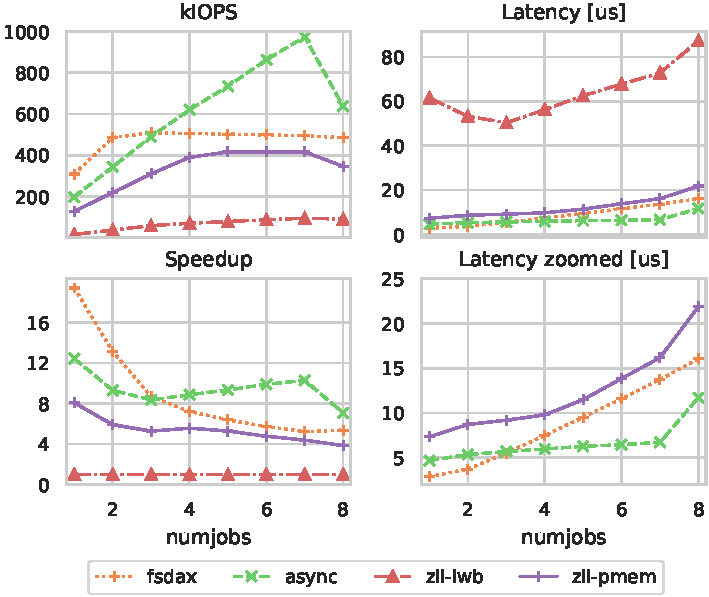
\includegraphics{fig/evaluation/fio4k__zilpmem_results}
    \caption{Mean IOPS and latency measured by \textit{fio} for our 4k synchronous random write workload, by number of writer threads (\lstinline{numjobs}).}
    \label{fig:eval:fio4k:metrics}
\end{figure}

We observed that the speedup for \lstinline{numjobs=1} and \lstinline{2} varies significantly between benchmark runs but remains stable for higher values of \lstinline{numjobs}.
We investigate this issue by computing the coefficient of variation (CoV) of the different configurations based on the mean and standard deviation of IOPS reported by fio ($\frac{stddev}{mean}$).
The results are displayed in Figure~\ref{fig:eval:fio4k:cov}:
The \textit{zil-pmem} CoV remains close to the CoV of \textit{async} until \lstinline{numjobs=4} from where it starts to decline towards the CoV of \textit{fsdax}.
This phenomenon correlates with the stop of increase in IOPS at \lstinline{numjobs=4}, supporting our assumption that \textit{zil-pmem}'s behavior is dominated by the PMEM hardware for numjobs 4--7.
In contrast, \textit{zil-lwb}'s CoV is 5x that of \textit{zil-pmem} for \lstinline{numjobs=1} and 2x for \lstinline{numjobs=2} before it starts to align closely with \textit{async}.
In absolute terms, for \lstinline{numjobs=1}, the standard deviation for ZIL-LWB is 4.7k IOPS with a mean value of merely 16k IOPS.
In contrast, for ZIL-PMEM, the standard deviation is 7.5k IOPS at a mean of 128k IOPS.

\begin{figure}[H]
    \centering
    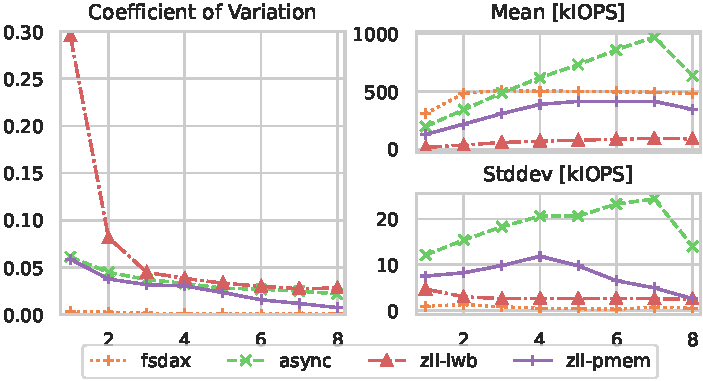
\includegraphics{fig/evaluation/fio4k__coefficient_of_variation.pdf}
    \caption{Comparison of the coefficient of variation ($\frac{stddev}{mean}$). The smaller plots display the absolute values.}
    \label{fig:eval:fio4k:cov}
\end{figure}

To understand ZIL-PMEM's impact on tail latencies, we compare the 5th, 95th, 99.9th, 99.9th, 99.99th and 99.99th's latency percentiles reported by fio.
\textit{zil-pmem} follows \textit{async} with a near-constant offset for all percentiles until \lstinline{numjobs=4} where we observe the characteristical ``knee in the curve'' which is to be expected given that the system's peak IOPS are first achieved at this value of \lstinline{numjobs}.
In contrast, \textit{zil-lwb}'s base latency (5th percentile, \lstinline{numjobs=1}) is $\frac{36.6}{6.7} [\frac{us}{us}] = 5.46$ times higher than \textit{zil-pmem}'s and the higher percentiles show a steeper growth with rising \lstinline{numjobs}.
Note that, by definition, the tail latencies for high percentiles at higher \lstinline{numjobs} only have proportional and thus minor impact on the CoV.

\begin{figure}[H]
    \centering
    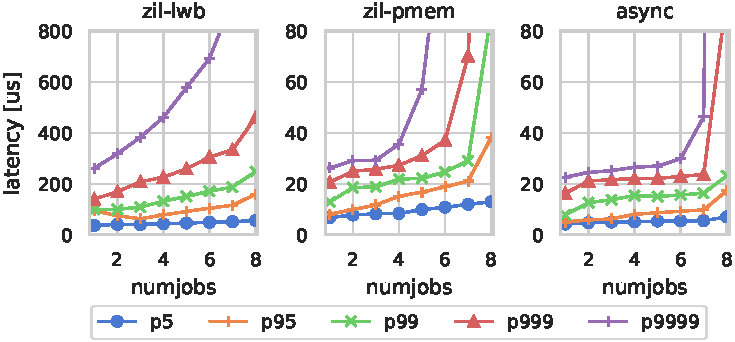
\includegraphics{fig/evaluation/fio4k__tail_latencies.pdf}
    \caption{Comparison of completion latencies by percentile. Note the different y-axis scales.}
\end{figure}

To get an idea of the distribution of per-IOP latency in ZIL-PMEM, we generalize our eBPF instrumentation from Section~\ref{ch:lwb_analysis:breakdown} to support both ZIL-PMEM.
We compare the results in Figure~\ref{fig:eval:fio4k:breakdown}.
The \lstinline{zil_persistence} component supersedes the ZIL-LWB specific ones: it is defined as the overall time spent in \lstinline{zil_commit} minus the time spent filling the commit list.

Whereas \lstinline{zil_persistence} is the dominant factor for latency in ZIL-LWB (80\% of average per-IOP latency, as observed in Section~\ref{ch:lwb_analysis:breakdown}), ZIL-PMEM only spends approximately 25\% on persistence to PMEM.
For ZIL-PMEM, the dominant component with more than 50\% is the \textit{async} code, i.e, VFS-level work and modification of in-DRAM DMU objects.
And in contrast to ZIL-LWB, the shared ITX code is a noticeable component at 10\%.
The absolute \textit{async} overhead for ZIL-PMEM is lower than for ZIL-LWB, particularly for small \lstinline{numjobs} values.
We have no satisfying explanation for this behavior.

\begin{figure}[H]
    \centering
    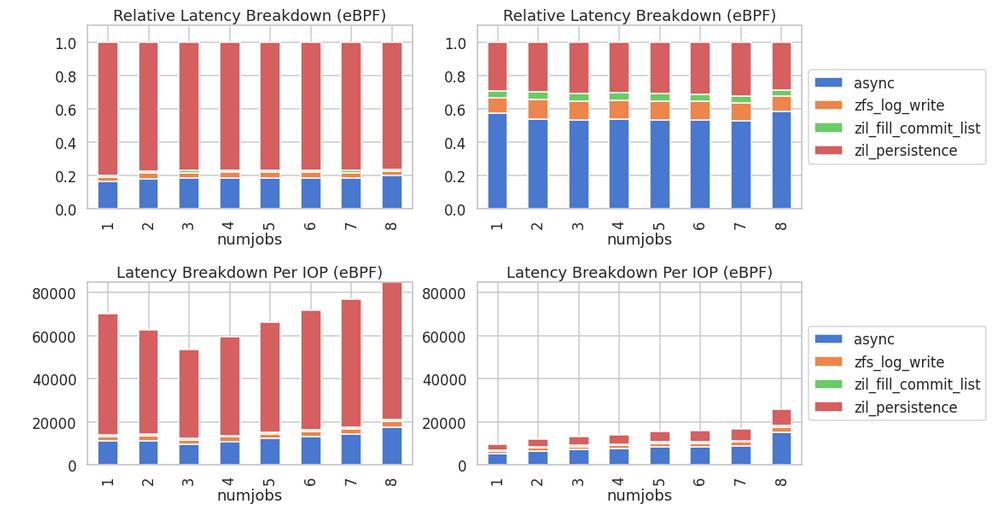
\includegraphics{fig/evaluation/comparison_zil_overhead_lwb_vs_pmem.pdf}
    \caption{
        Comparison of relative and absolute latency contribution of functions executed by fio threads when they perform synchronous writes.
    }
    \label{fig:eval:fio4k:breakdown}
\end{figure}

\subsection{Application Benchmarks}\label{sec:eval:appbenchmarks}
We determine ZIL-PMEM's impact on real-world application performance using additional macro-level and application-level benchmarks.
We execute each benchmark on top of different \textit{storage stacks} that represent alternatives to ZIL-PMEM and compare the results in the subsequent sections.

We define a \textit{storage stack} as a configuration of storage hardware and software that exposes a filesystem at a mountpoint $M$.
Executing a benchmark \textit{on top of} a storage stack means that the benchmark is configured to place all of its data within the filesystem mounted at $M$.
We define the following storage stacks.
\begin{description}[noitemsep,leftmargin=1.5cm,labelindent=1cm]
    \item[zfs-\{lwb,pmem,async\}] A \underline{\smash{\smash{single}}} ZFS dataset created on a zpool with the familiar hardware configuration (30 striped NVMe partitions and /dev/pmem0 as SLOG).
        For \textit{zfs-lwb} and \textit{zfs-pmem}, we configure the corresponding ZIL kind.
        For \textit{zfs-async}, we configure the ZIL-LWB ZIL kind but set the \lstinline{sync=disabled} property.
        All variants use a \lstinline{recordsize=4k} and \lstinline{compression=off} on the dataset since most of our benchmarks are synchronous workloads with small write sizes.
        For the \textit{zil-pmem} variant, we configure PRB with \lstinline{ncommitters=3}.
    \item[\{xfs,ext4\}\{,-dax\} on \$BDEV] Linux 5.9's \textit{xfs} or \textit{ext4} filesystems deployed on the \textit{block device stack} \lstinline{$BDEV}.
        If the ``\textit{-dax}'' suffix is present, the \lstinline{dax} mount option was set.
        We always perform benchmark runs without DAX, and perform an additional run if \lstinline{$BDEV} is a DAX-capable device.
\end{description}
The \textit{xfs} and \textit{ext4} stacks are parametrized by the \textit{block device stack} \lstinline{$BDEV} which we define as a hardware and software configuration that provides a (potentially virtual) block device.
We define the following block device stacks:
\begin{description}[noitemsep,leftmargin=1.5cm,labelindent=1cm]
    \item[devpmem] The raw \lstinline{fsdax} namespace block device in devfs (/dev/pmem0).
    \item[dm-writecache]
        The \textit{dm-writecache} Linux Device Mapper target synchro\-nously persists writes to a cache device and performs asynchronous write-back to an origin block device in the background.
        It has explicit support for DAX devices.
        We configure \textit{dm-writecache} with \mbox{/dev/pmem0} as the cache device and a \textit{dm-stripe} of the 30 NVMe partitions as the origin data store.
        Since most benchmarks consume relatively little space compared to /dev/pmem0's capacity (40GiB), we set the \textit{low watermark} parameter to 0\% and \textit{high watermark} to 1\% in order to trigger some write-back during benchmark execution.
        (Refer to Section~\ref{sec:cross_media_storage_systems} for details on \textit{dm-writecache}.)
    \item[zvol-lwb,rs=\{0,1\}]
        A ZVOL exposed by a zpool in the same config as \textit{zfs-lwb}.
        We set \lstinline{volblocksize=4k} on the ZVOL dataset.
        The \textit{rs} variable controls the value of the \lstinline{zvol_request_sync} tunable which, if enabled, processes block IO requests (\lstinline[style=figurepseudocode]{struct bio}) synchronously instead of submitting them to a thread pool.
        (Refer to Section~\ref{sec:itxgbypass:openzfsbackground_zvols} for more details on ZVOLs.)
    \item[zvol-async] Like \textit{zvol-lwb} but with \lstinline{sync=disabled}.
    \item[zvol-pmem,rs=\{0,1\},byp=\{0,1\}] Like \textit{zvol-lwb} but with the ZIL-PMEM ZIL kind.
        PRB's \lstinline{ncommitters} tunable is always set to $3$.
        The \textit{byp} variable controls whether the ITXG bypass is enabled (0 disabled, 1 enabled).
\end{description}
The following items are examples for storage stacks used in the evaluation:
\begin{description}[noitemsep,leftmargin=1.5cm,labelindent=1cm]
    \item[ext4 on zvol-pmem,rs=1,byp=0] Ext4 deployed on a ZVOL on a zpool with the ZIL-PMEM ZIL kind.
        \lstinline{zvol_request_sync} is set, the ITXG bypass is disabled, and \lstinline{ncommitters} is set to \lstinline{3}.
        The ext4 file system is mounted without the \lstinline{dax} mount option.
    \item[xfs-dax on devpmem] XFS deployed directly on the PMEM block device (/dev/pmem0).
    It is mounted with the \lstinline{dax} option.
    \item[zfs-pmem] ZFS with the ZIL-PMEM ZIL kind and the default value of \lstinline{ncommitters=3}.
        \lstinline{Zvol_request_sync} and the ITXG bypass are only relevant for ZVOLs and therefore are not part of the configuration name.
\end{description}

We compare the performance of the storage stacks with the set of benchmarks described below.
To facilitate the comparison, all benchmarks have the following properties:
\begin{description}[noitemsep,leftmargin=1.5cm,labelindent=1cm]
    \item[Scaling Factor] The scaling factor increases the degree of concurrent synchronous IO operations issued by the benchmark.
        We run each benchmark with three scaling factor values: 1, 4, and~8.
    \item[Result Metric] Each benchmark reports a single result metric per run.
        This allows us to compare performance across different storage stacks and scaling factor values.
        For all benchmarks in this evaluation, a numerically greater result is better.
\end{description}
What follows is a description of the benchmarks:
\begin{description}[noitemsep,leftmargin=1.5cm,labelindent=1cm]
    \item[fio-growing] The 4k synchronous random write workload that motivated our work, but with all worker thread files within the same filesystem.
        The scaling factor maps to the \lstinline{numjobs} parameter which controls the number of worker threads.
        The working set (amount of modified data) grows with the scaling factor because each additional thread adds a private file with a constant size of 100~MiB.
        We report mean IOPS as the result metric.

    \item[fio-fixed] The 4k synchronous random write workload, with all files on a single filesystem, but a fixed working set size, independent of \lstinline{numjobs}.
        We achieve the fixed working set size by setting the \lstinline{size} parameter to $\frac{1~\text{GiB}}{numjobs}$.
        We report mean IOPS as the result metric.

    \item[filebench varmail] Filebench is a benchmark execution engine that allows for definition of workloads in a domain-specific language.
        The pre-defined \textit{varmail} workload
        ``emulates I/O activity of a simple mail server that stores each e-mail in a separate file (/var/mail/ server).
          The workload consists of a multi-threaded set of create-append-sync, read-append-sync, read and delete operations in a single directory.
        ''~\cite{FilebenchGitHubWiki}.
        We use filebench in version \lstinline{1.5-alpha1-33-g22620e6} with the upstream workload definitions.
        The scaling factor maps to the workload's \lstinline{$nthreads} variable which determines the number threads that execute the operations described above.
        We use a runtime of 20 seconds per configuration and report filebench's \textit{ops per second} value as the result metric.

    \item[filebench oltp] The filebench \textit{oltp} workload emulates database workloads.
        It ``performs file system operations using Oracle 9i I/O model.
        It tests the performance of small random reads and writes, and is sensitive to the latency of moderate size (128k+) synchronous writes to the log file.
        By default [it] launches 200 reader processes, 10 processes for asynchronous writing, and a log writer.''~\cite{FilebenchGitHubWiki}.
        We leave all parameters at the default setting except for the \lstinline{$ndbwriters} parameter for which we use the scaling factor's value instead of its default value of ten.
        It is our understanding that scaling the number of log writer threads to a number greater than one would not be feasible with the real DBMS and thus be unrealistic.
        We use a runtime of 20 seconds and report filebench's \textit{ops per second} value as the result metric.

    \item[MariaDB/sysbench] We deploy the MariaDB 10.5.9 Docker image in its default configuration (InnoDB storage engine) with the /var/lib/mysql directory bind-mounted to a sub-directory within the storage stack's mountpoint.
        We apply the \textit{sysbench} benchmark's \textit{oltp\_insert} workload with its default parameters for ten seconds.
        The workload spawns a number of threads that inserts rows with random data into one or more tables.
        We use the default setting (a single table) and map the scaling factor to the number of threads that perform the insert queries.
        Each thread uses a private, long-lived connection to the MariaDB server.
        We use Docker's \lstinline{--net=host} parameter when starting the MariaDB container to allow sysbench to connect via loopback TCP, avoiding the overhead of Docker's user-space proxy.
        The result metric is the number of transactions per second (tps) reported by sysbench.

    \item[Redis-SET] Redis is a popular in-memory key value store.
        For persistence, it provides two mechanisms that are recommended to be used in combination.
        First, the system periodically persists a snapshot of the Redis database (RDB).
        This process happens in the background in a forked child process.
        Second, Redis features a logical write-ahead log (\textit{append-only file}, AOF) that is extended for every mutating operation and replayed after a crash.
        Redis supports three different behaviors for ensuring durability of the AOF, configurable through the \lstinline{appendfsync} configuration variable.
        A value of \lstinline{no} does not perform any fsyncs, \lstinline{everysec} performs an fsync every second (default), and \lstinline{always} performs an fsync operation for operation logged to AOF.
        \cite{RedisPersistenceRedis}

        We deploy Redis 6.2 (built from source).
        We configure RDB writeback to happen every second, regardless of the number of changes,
        We enable AOF and configure \lstinline{appendfsync=always} which effectively turns our Redis deployment into a durable key-value store.

        For benchmarking, we use Redis's own \textit{redis-benchmark} tool~\cite{HowFastRedis}.
        The scaling factor maps to the \lstinline{--threads} and \lstinline{-c} parameters which control the number of parallel clients.
        We use the benchmark's \textit{SET} workload to perform $10^6$ \textit{SET} operations with random keys and the default value size (3 bytes).
        We configure a keyspace size of $10^6$  to reduce contention.
        We leave the values for pipelining and connection keepalive at their defaults (no pipelining, keepalive enabled).
        The result metric is the requests-per-second (rps) value reported by redis-benchmark.

        We choose the number of $10^6$ \textit{SET} operations because it results in runtimes of ten seconds or more for most combinations of scaling factor and storage stacks.
        The only exception is \textit{zfs-async} for which the shortest runtime is 8~s.

    \item[RocksDB-fillsync] RocksDB is a popular key-value store developed by Facebook that is optimized for fast storage devices.
        It can be used directly by applications as an embedded database but is also the basis for the \textit{MyRocks} storage engine for MySQL~\cite{MyRocksRocksDBStorage}.
        % RocksDB mainline supports PMEM as a LRU cache and several academic publications have proposed deeper PMEM integration.\todo{need to cite it}
        RocksDB uses log-structured merge trees for long-term storage which are written and rewritten in large units that are prepared in DRAM (memtables).
        Operations that request synchronous semantics using the \lstinline{WriteOptions.sync} flag are logged to a write-ahead log file.~\cite{FlushWALLessFwrite,RocksDBGitHubWikiWalPerformance}

        We measure the impact of ZIL-PMEM on RocksDB WAL performance with the \textit{fillsync} benchmark that is part of RocksDB's \textit{db\_bench} tool.
        \textit{Fillsync} performs a fixed number of synchronous \textit{Put} operations with random keys.
        We set the number of operations to 400k and map the scaling factor to the number of concurrently \textit{Put}ting threads.
        The result metric is the \textit{ops-per-sec} (operations per second) value reported by \textit{db\_bench}.

        We choose the number of 400k operations because it results in at least ten seconds of runtime for 90\% of configurations.
        The configurations that achieve less than ten seconds of runtime are:
        \begin{itemize}[noitemsep]
            \item All \textit{zfs-pmem} configurations at scaling factor $1$ ($\sim$4~s runtime)
            \item \textit{zfs-async} for scaling factors $1, 4, 8$ (${\sim}2$, $6.8$ and 8~s rt.)
            \item \textit{xfs-on-devpmem} with \lstinline{dax} mount option at scaling factor $1$ (9.1~s~rt.)
        \end{itemize}
\end{description}

\subsubsection{ZIL-PMEM vs. ZIL-LWB}\label{sec:eval:zilpmemvslwb}

\begin{figure}[H]
    \centering
    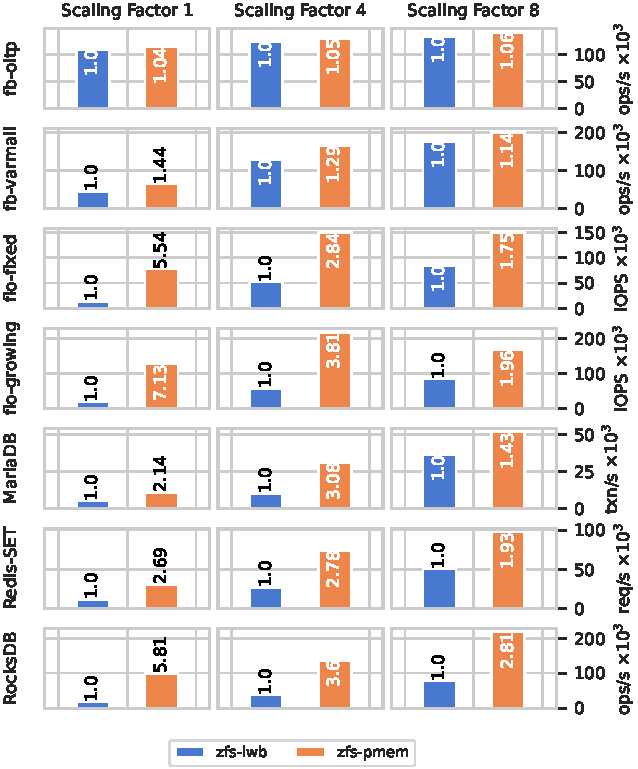
\includegraphics{fig/evaluation/appbench__zilpmem_vs_lwb.pdf}
    \caption{App Benchmarks: ZIL-PMEM vs. ZIL-LWB. The number on each bar indicates the speedup over \textit{zfs-lwb}.}
    \label{fig:eval:appbenchmarks:zilpmem_vs_zilllwb}
\end{figure}

We first compare the speedup of ZIL-PMEM over ZIL-LWB.
ZIL-PMEM outperforms ZIL-LWB in all benchmarks, but the speedup varies significantly for the different workloads and scaling factors.
The highest speedups are achieved at scaling factor $1$ by the fio workloads (7.13x, 5.54x) and \textit{RocksDB-fillsync} (100k ops-per-sec, a speedup of 5.8).
\textit{Redis-SET} achieves shows a speedup of 2.69 (30k rps) and MariaDB achieves 10k tps which is a speedup of 2.14.
For scaling factor $4$, the fio and RocksDB's speedup declines whereas Redis's grows to 2.78 and MariaDB's grows to 3.08.
For scaling factor $8$, all workloads show a reduction in speedup (RocksDB 2.81x, Redis 1.93x, MariaDB 1.43x).

The \textit{filebench-oltp} workload shows no relevant speedup or slowdown for all scaling factor values.
We observed during benchmark execution that the 200 reader processes always cause 100\% CPU utilization.

The \textit{filebench-varmail} workload only shows a speedup of 1.43 at scaling factor $1$ which shrinks to 1.14 at scaling factor $8$.
A possible explanation for these meager results is the larger data volume (16k appends) compared to the fio workloads (4k writes).
In combination with the large amount of metadata (file creation and deletion), ZIL-LWB might also be benefitting from the \textit{commit ITXs'} pipelininig.
In any way, \textit{filebench-varmail} shows that the large speedups for small writes cannot be generalized to all filesystem workloads.
Future work should investigate ZIL-PMEM's behavior during this benchmark in detail and determine how beneficial pipelining akin to \textit{commit ITXs} could be.

\subsubsection{ZIL-PMEM vs. XFS and Ext4 on PMEM}

Our next set of results is the comparison between the Linux filesystems XFS and Ext4 and ZFS with both ZIL kinds (\textit{zfs-lwb}, \textit{zfs-pmem}).
We also include \textit{zfs-async} as a theoretical upper bound for any ZIL kind.
Since both XFS and Ext4 are DAX-aware, we inlcude configurations with and without the \textit{dax} mount option.
%Note that, since the ZIL unconditionally journals all data, including file contents, the \textit{lwb} and \textit{pmem} ZFS configurations provide significantly stronger crash consistency guarantees than the Linux filesystems which only journal metadata.
%Nope, that argument is moot because all workloads use fsync and all the filesystems impmlement it correctly (hopefully).
Note that that the ZFS configurations only use PMEM for the ZIL but NVMe devices for permanent storage whereas the Linux filesystem configurations are PMEM-only.

\begin{figure}[H]
    \centering
    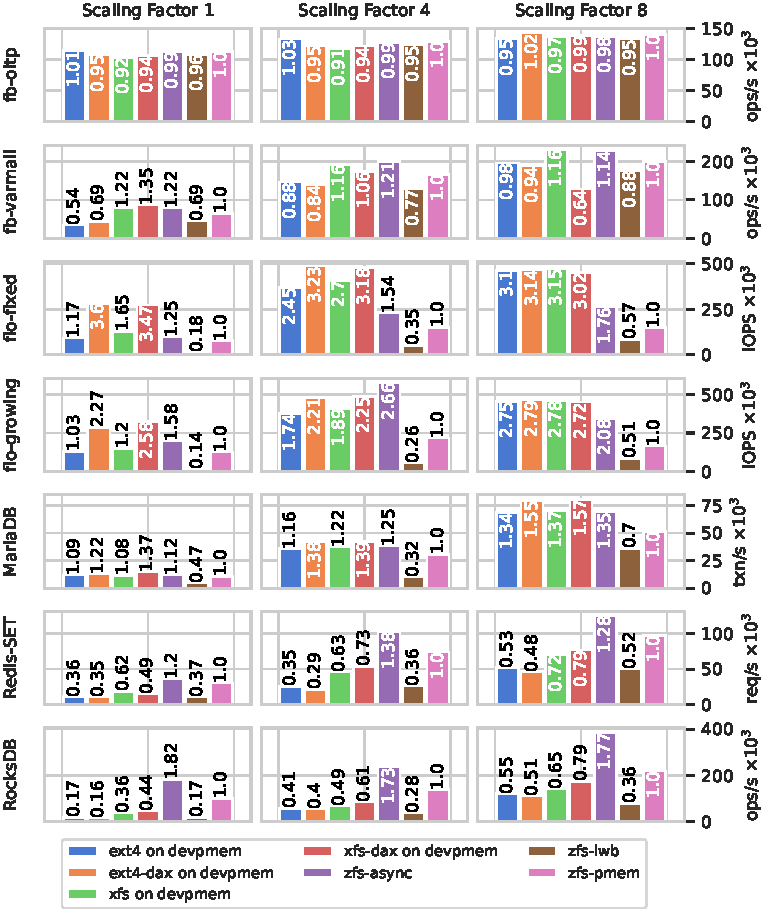
\includegraphics{fig/evaluation/appbench__zfs_vs_linuxfs_on_pmem.pdf}
    \caption{
        ZFS with ZIL-PMEM, ZIL-LWB and \lstinline{sync=disabled} (\textit{zfs-async}) as well as ext4 and xfs on /dev/pmem, with and without the \textit{dax} mount option.
        The number on each bar indicates the speedup over \textit{zfs-pmem} in the respective benchmark \& scaling factor.
    }
\end{figure}

Our primary takeaway from this comparison is that, in contrast to ZIL-LWB, ZIL-PMEM is competitive with both ext4 and xfs at scaling factor $1$ in most benchmarks.
The fio workloads are the exception, where the Linux filesystems achieve a speedup of greater than 3 if the \textit{dax} mount option is enabled.
The reason for this phenomenon is most likely lower CPU overhead at scaling factor $1$ (compare \textit{zfs-pmem} with \textit{zfs-async}), and better multi-core scalability at higher scaling factors.
Note that, since the benchmarks in this section all write to a single dataset, ZIL-PMEM's scalability is bounded by the sequential logical structure of the ZIL.

ZIL-PMEM performs exceptionally great for the \textit{Redis-SET} and \textit{RocksDB-fillsync} workloads at all scaling factors.
The write-ahead log files written that these workloads write are consists of encoded representation of logical changes.
The mutating requests issued by our benchmarks have small payloads and result in small \lstinline{write+fsync} system calls.%
\footnote{
    The RocksDB documentation and comments in the source code suggest that the WAL files are written in 32k blocks that are zero-padded if necessary~\cite[db/log\_writer.h]{RocksDBGitHubWikiWalPerformance}.
    We observed the contrary behavior with \lstinline{strace}: each \textit{Put} operation with \lstinline{WriteOptions.sync} results in a \lstinline{write} and \lstinline{fdatasync} system call. The \lstinline{write} system call's data size is proportional to the sum of the \textit{Put} operation's key and value sizes.
}
We assume that ZIL-PMEM handles this IO pattern more efficiently than the Linux filesystems.
First, in non-DAX mode, every small append + fsync operation on the Linux filesystems is necessarily amplified to block granularity, both for the data that is modified in place and for metadata that is additionally journaled.
In contrast, ZIL-PMEM's PMEM write volume per append+fsync is most likely smaller.
For example, a PRB entry for a small write system call only consumes $256 + 256 \times \lceil \frac{192 + size}{256} \rceil$ bytes of PMEM.
Second, even in DAX-aware mode, the implementations of Ext4 and XFS still assume block devices as the storage medium for their JBD2 journal (Ext4) or write-ahead log (XFS).
Thus, both write amplification and unnecessary disk-oriented optimizations might be relevant here.

In the \textit{MariaDB} benchmark, the DAX-aware Linux filesystems achieve up to 1.57x more transactions per second than ZIL-PMEM.
\textit{Zfs-async} and the the non-DAX-aware configurations achieve 1.12x, 1.25x and 1.35x higher results at scaling factors 1, 4, and 8.
Manual inspection of the CPU utilization shows a significant amount of context switching but no clearly identifiable CPU bottleneck.
% strace -e pwrite64,fdatasync -f -p $(pgrep mysqld)     
% ls -lah /proc/$(pgrep mysqld)/fd                       
% => mostly 1024B writes to ib_logfile0 which according to https://mariadb.com/kb/en/innodb-redo-log/ is the redo log file
The database server process performs 1024 byte sized \lstinline{write} + \lstinline{fdatasync} system calls to the InnoDB redo log file from a single thread.
However, since \textit{zfs-async} does not perform better than any of the systems that actually write to PMEM, we can rule out PMEM bandwidth as a possible bottleneck.

Regarding the \textit{filebench-oltp} benchmark, no configuration performs exceptionally better than any other, including \textit{zfs-async}.
We observe high CPU utilization in all benchmark configurations, caused by the ``hog'' stage of the 200 processes that the benchmark uses to simulate reader threads.
Thus, CPU time is most likely the bottleneck in all configurations.

For \textit{filebench-varmail}, the highest speedup over ZIL-PMEM is 1.35 at scaling factor $1$, achieved by XFS in DAX-aware mode, followed by ZFS with \textit{zfs-async} with 1.22x.
For higher scaling factors, XFS's speedup diminishes and even goes below 1 at scaling factor $8$, albeit only in DAX-aware mode.
We have no satisfying explanation for this behavior.
Also, the fact that \textit{zfs-async} achieves a lower speedup than XFS can be taken as an indicator that \textit{filebench-varmail} is not bound by PMEM performance, contradicting our speculation in the previous section.

\subsubsection{ZIL-PMEM vs. XFS and Ext4 on Dm-writecache}\label{sec:eval:dmwritecache}

The comparison between ZIL-PMEM with NVMe storage and Linux filesystems on pure PMEM in the previous section is insightful but not a level comparison in terms of storage hardware performance and available functionality.
A more practically relevant competitor to ZIL-PMEM is \textit{dm-writecache} with a \textit{dm-stripe} of NVMe partitions as the origin block device.
In this section, we compare ZFS with ZIL-PMEM and ZIL-LWB to Ext4 and XFS on such a setup.

\begin{figure}[H]
    \centering
    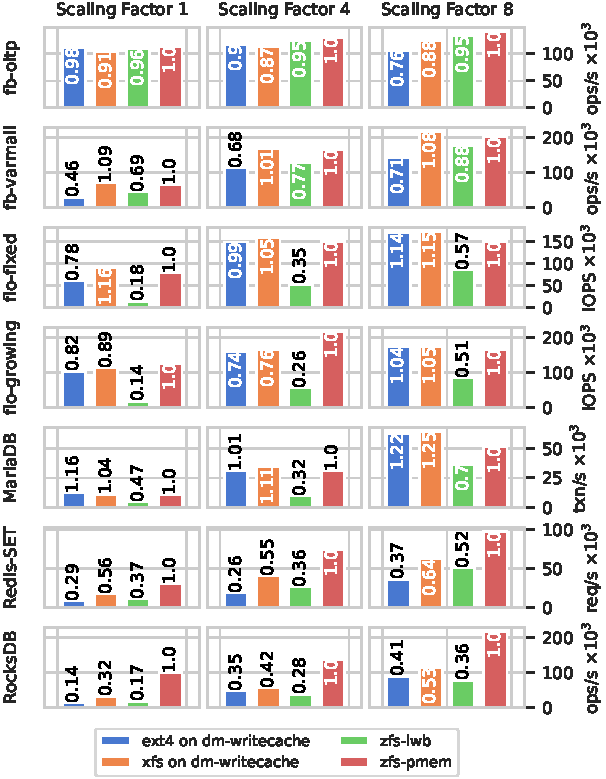
\includegraphics{fig/evaluation/appbench__dm_writecache.pdf}
    \caption{
        Comparison of the benchmark results for ZIL-PMEM and ZIL-LWB vs. Linux filesystems on dm-writecache.
        The number on each bar indicates the speedup over \textit{zfs-pmem} in the respective benchmark \& scaling factor.
    }
\end{figure}

ZIL-PMEM's performance is within +/-30\% of XFS on \textit{dm-writecache} at all scaling factors in all benchmarks except \textit{Redis-SET} and \textit{RocksDB-fillsync} where ZIL-PMEM performs significantly better.
The 30\% spread decreases slightly with higher scaling factors but does not change the overall picture.
Our explanation for ZIL-PMEM's significantly better performance in the \textit{Redis-SET} and \textit{RocksDB-fillsync} workloads is (again) write amplification, possibly combined with the suboptimal scaling behavior of dm-writecache that we describe below.

Ext4 performs significantly worse than ZIL-PMEM (and XFS!) in some benchmarks, with only 46\%, 29\%, and 14\% of ZIL-PMEM's performance in \textit{filebench-varmail}, \textit{Redis-SET}, and \textit{RocksDB-fillsync} at scaling factor~1.
Write amplification might be a possible explanation as well.

We have observed the system while benchmarking the \textit{dm-writecache} stack to ensure that the comparison with ZFS is actually fair.
We found that, despite the very aggressive write-back configuration (high watermark = 1\%, low watermark = 0\%), the system performed very little write-back to the NVMe drives.
The two \textit{fio} workloads were the exception, but the write load towards the NVMe devices was well below their maximum capacity.
Thus, NVMe was not a bottleneck in the benchmark.
However, we found that \textit{dm-writecache} has severe multi-core scalability problems.
For example, XFS on raw PMEM without the \textit{dax} mount option achieves 150k IOPS at scaling factor 1 and 409k IOPS at scaling factor 4 in the \textit{fio-growing} workload.
In contrast, on dm-writecache, it is 112k IOPS at scaling factor 1 but only 165k IOPS at scaling factor 4.
Using the \textit{perf} tool, we observed severe contention at a lock that serializes access to the entire dm-writecache instance's state.
In private communication, dm-writecache's maintainer Mikulas Patocka stated that ``the purpose of dm-writecache is to decrease commit latency, not to increase throughput. There is not much that can be done with the lock contention''.
ZIL-PMEM has similar problems in \textit{fio-growing} (125k IOPS at factor 1, 217k at factor 4) albeit due to the sequential structure of ZIL chain, not the scalability of PRB/HDL.
(We know from Section~\ref{sec:eval:4ksyncwrites} that we can achieve 400k IOPS with \lstinline{numjobs} / scaling factor 4 if each writer thread operates on a seprate dataset.
 However, remember that for comparability with the Linux filesystems, the \textit{fio-fixed} and \textit{fio-growing} workloads operate on a single ZFS dataset when executed on a zfs-\* stack.)
In the next section, we investigate whether a more relaxed log structure such as the ITXG bypass can improve this shortcoming of the ZIL structure.

%Note that even though the Linux filesystem are DAX-aware, this functionality cannot come to fruition on top of \textit{dm-writecache}.
%This highlights a fundamental advantage of ZFS's integrated design (filesystem and volume manager) which, with ZIL-PMEM, is \textit{both} optimized for PMEM \textit{and} provides a rich set of additional functionality such as redundancy via mirroring or raidz, checksumming, and encryption.

\subsubsection{Impact on ZVOL Performance \& ITXG Bypass}\label{sec:eval:zvols_ad_itxg_bypass}

In this section, we examine the impact of ZIL-PMEM on ZVOLs.
We compare the performance of XFS deployed on a ZVOL in a zpool with varying ZIL kinds, \lstinline{zvol_request_sync} (\lstinline|rs_{0,1}|), and ITXG bypass setting (\lstinline|byp_{0,1}|).
The results are relative to \textit{zvol-pmem,rs=0,byp=0} as the baseline which is the standard configuration for ZIL-PMEM pools.
Note that deploying a filesystem on a ZVOL generally makes little sense in practice because ZFS filesystems provide the same basic service with more additional features at less overhead.
However, ZVOLs are a popular choice for storage virtualization where ZVOLs are used as virtual hard disks, either on the same host or via a SAN (e.g., iSCSI, Fibre Channel).
To simplify our evaluation, we avoid the overhead of a hypervisor or SAN and instead instantiate XFS directly on top of the ZVOL, mount it, and execute the benchmarks.

\begin{figure}[H]
    \centering
    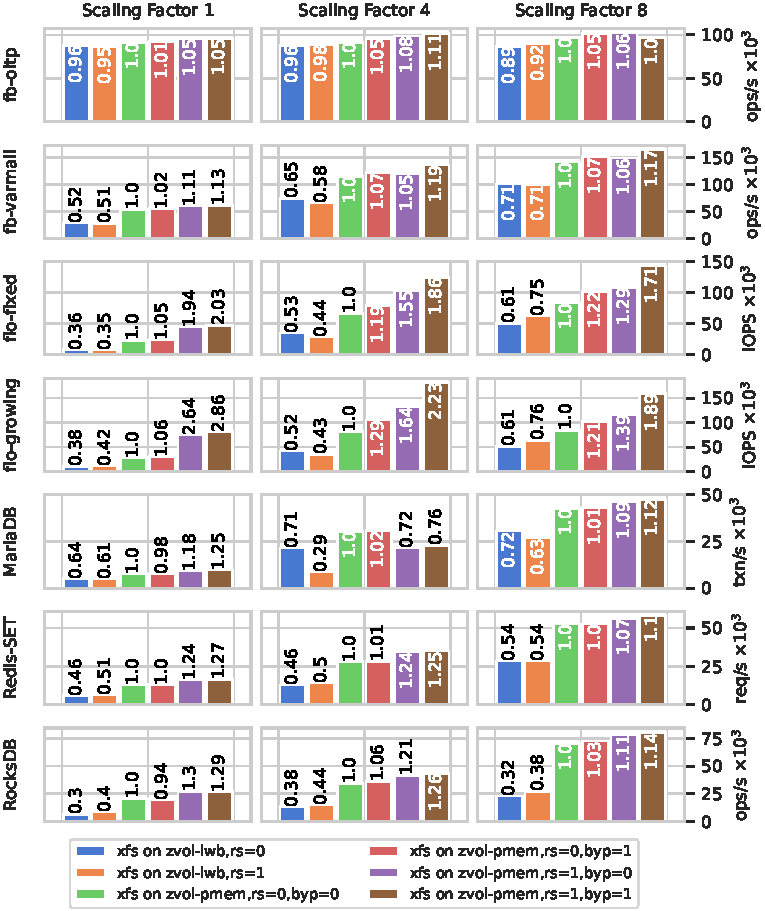
\includegraphics{fig/evaluation/appbench__xfs_zvol.pdf}
    \caption{
        Comparison of the benchmark results for XFS on ZVOLs on different zpool configurations.
        The number on each bar indicates the speedup over ZIL-PMEM in the \textit{zvol-pmem,rs=0,byp=0} configuration.
    }
\end{figure}


Our first observation is that the default configuration of ZIL-PMEM, \textit{rs=0,byp=0}, delivers a significant speedup over ZIL-LWB.
At scaling factor 1, it is approximately 2x for all workloads except \textit{MariaDB} ($\frac{1}{0.64} = 1.56$) and \textit{filebench-oltp} ($\frac{1}{0.96} = 1.04$).
At higher scaling factors, the speedup declines for all benchmarks albeit less so with \textit{Redis-SET} and \textit{RocksDB-fillsync} than with the other workloads.

The effect of \lstinline{zvol_request_sync=1} is ambiguous and not very signficant for ZIL-LWB but very beneficial for ZIL-PMEM in the \textit{fio} workloads at scaling factor 1 with a 2x and 2.6x speedups over the standard configuration, respectively.
\textit{MariaDB}, \textit{Redis-Set} and \textit{RocksDB-fillsync} also benefit with speedups of 1.18x, 1.23x, and 1.30x over the default configuration.
However, for scaling factor 4, \textit{MariaDB} performs substantially worse if \lstinline{zvol_request_sync} is set (30k tps vs. 20k tps).
We also conducted the benchmarks with Ext4 instead of XFS (not shown in the plot).
Ext4 exhibited worse performance in almost all configurations if \lstinline{zvol_request_sync} was set, with the exception of the \textit{fio} workloads.

The ITXG bypass only has marginal effects with and without \lstinline{zvol_request_sync}, except for the \textit{fio} workloads at scaling factors 1 and 4.
For example, \textit{fio-growing} at scaling factor 8 shows an increase in IOPS from 84k to 102k (21\%) for \textit{rs=0} and from 117k to 159k (35\%) with \textit{rs=1}.
For Ext4, \textit{filebench-varmail} also shows a 20\% improvement with enabled ITXG bypass (\textit{byp=1}) and \textit{rs=0}.
Activation of the ITXG bypass does not appear to have a negative impact for XFS in the remaining workloads.
For Ext4, we observed some performance degradatations in setups whether both ITXG bypass and \lstinline{zvol_request_sync} were enabled.

In summary, ZIL-PMEM provides a signficant performance advantage for ZVOLs but is less effective than with ZFS filesystems (see Sections~\ref{sec:eval:4ksyncwrites} and \ref{sec:eval:zilpmemvslwb}).
This is particularly noticeable in the \textit{fio} workloads and \textit{RocksDB-fillsync}.
Their speedup with ZIL-PMEM on XFS+ZVOL is only half the speedup of what we observed for ZFS at scaling factor~1.
Write amplification cannot be responsible for this behavior because fio already writes at 4k block size.
The most likely cause is latency overhead added by the filesystem that affects all workloads equally.

\subsection{CPU-Efficient Handling Of PMEM Bandwidth Limits}\label{sec:eval:ncommitters_scalability}

PRB's \textit{commit slot} mechanism limits the amount of parallel writers to PMEM to \lstinline{ncommitters}.
The goal is to avoid wasteful on-CPU stall cycles which inevitably occur if the aggregate write bandwidth to PMEM exceeds the hardware capacity.
(See Sections~\ref{sec:requirements} and \ref{di:prb:write} for a more detailed explanation.)

To determine the mechanism's effectiveness, we use our 4k synchronous random write workload with \underline{\smash{separate}} ZFS filesystems per fio thread.
We add low-overhead per-CPU counters to ZIL-PMEM to sum up the total mount of time that is spent writing PMEM ($T_{pmem}$), as well as the number of write operations performed during the benchmark ($N_{ops}$).
We then compute the \textit{average PMEM write time per IOP} $T_{pmem_{iop}} = \frac{T_{pmem}}{N_{ops}} [\frac{s}{op}]$.
The most efficient value for \lstinline{ncommitters} for a given system depends on the workload and efficiency goals.
In general, \lstinline{ncommitters} should be the minimal value where $T_{pmem_{iop}}$ is tolerable but the system's primary performance metric is not impacted.

We compute $T_{pmem_{iop}}$ for 1 to 18 numjobs, different values of \lstinline{ncommitters} and two different PMEM configurations.
The first PMEM configuration is a single, non-interleaved Optane DIMM.
The second configuration are four interleaved Optane DIMMs.
Regardless of how interleaving is configured, we create a 40~GiB-sized \textit{fsdax} namespace on the resulting region and use it as the PMEM SLOG for ZIL-PMEM.
We use a machine with higher core count for the benchmarks.
The system configuration is as follows:
\begin{description}[noitemsep,leftmargin=1.5cm,labelindent=1cm]
    \item[System] Supermicro SYS-1029U-TRT
    \item[Mainboard] Supermicro X11DPU, Version 1.10
    \item[CPU] 2 x Intel(R) Xeon(R) Gold 5220 CPU \@ 2.20GHz \\
        18 cores per socket, 2-way SMT per core
    \item[DRAM] 12 x 32GiB SK HYNIX DDR4-2666, HMA84GR7CJR4N-VK  % sudo dmidecode | grep -C8 DRAM | grep 'Part Number'
    \item[PMEM] 8 x Intel Optane DC Persistent Memory, 128 GB, (NMA1XXD128GPS), 4 per socket.
    \item[NVMe] System rootfs only, no dedicated NVMe hardware.
    \item[Kernel] Linux Kernel, Fedora 5.11.15-100.fc32.x86\_64
    \item[Userland] Fedora 32
    \item[fio] fio-3.21
\end{description}
As with our main evaluation system (described in Section~\ref{ch:lwb_analysis:setup}), we leave SMT enabled.
We disable the second socket in software using the \lstinline{isolcpus=18-35,54-71} kernel command line parameter.
Since the system does not have NVMe devices available, we provision the disabled socket's Optane DIMMs in non-interleaved mode, i.e., one PMEM region and a single \lstinline{fsdax} namespace per DIMM.
We use these namespaces as the zpool's main (non-SLOG) VDEVs.
% NOTE: we use \lstinline / ttt for ncommitters and math-mode for numjobs. 

\begin{figure}
    \centering
    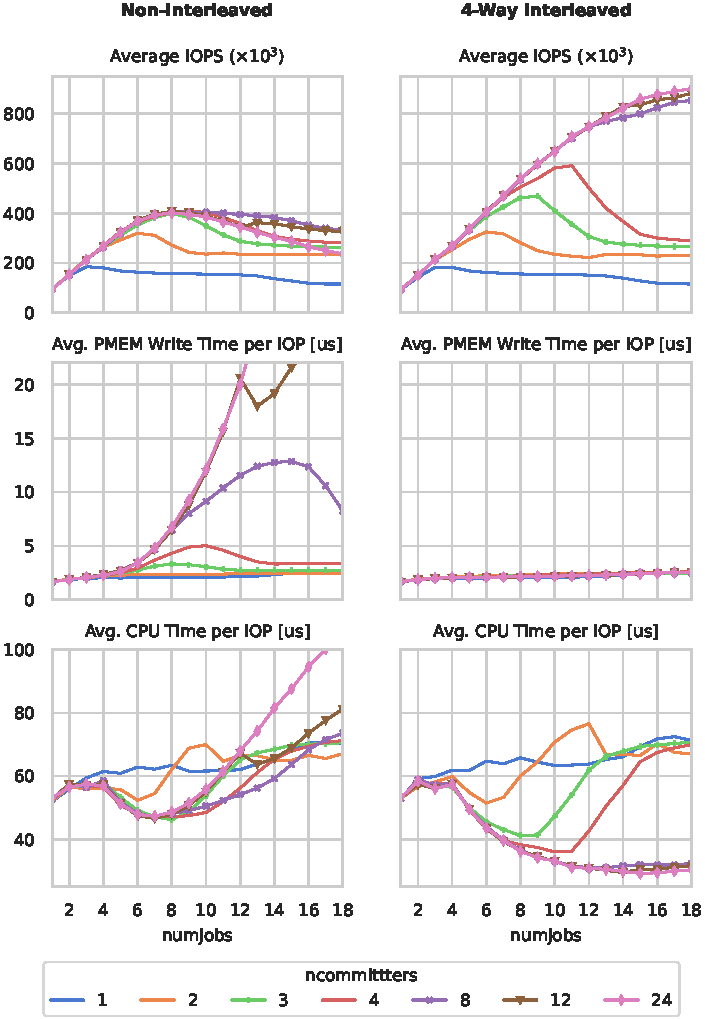
\includegraphics{fig/evaluation/ncommitters_scalability__comparision.pdf}
    \caption{Comparison of performance and PMEM write time per IOPS for different values of \lstinline{ncommitters} in the two PMEM configurations.}
    \label{fig:eval:ncommitters_scalability:main}
\end{figure}


Figure~\ref{fig:eval:ncommitters_scalability:main} visualizes the results of this experiment.
For the non-interleaved configuration, we observe that the system's peak IOPS is 400k, first achieved with \lstinline{ncommitters=3}.
For \lstinline{ncommitters=3}, IOPS quickly decline to 263k IOPS for higher $numjobs$.
With \lstinline{ncommitters=8}, the system is able to sustain the 400k IOPS for the for $numjobs \in 7 \dots 13$.
The price is significantly more on-CPU PMEM time per IOP:
looking at $numjobs = 8$, the $T_{pmem_{iop}}$ is $3.3, 4.3, 6.5~\text{us}$ for \lstinline{ncommitters=3}, \lstinline{4} and \lstinline{8}.
And at $numjobs = 12$, $T_{pmem_{iop}}$ climbs to $11.6, 20.6~\text{us}$ for \lstinline{ncommitters=8} and \lstinline{12} whereas \lstinline{ncommitters=3} is successfully limited to $2.7~\text{us}$ of PMEM write time per IOP.
The \lstinline{ncommitters=12} and \lstinline{24} configurations do not achieve higher peak IOPS than \lstinline{ncommitters=8} but decline to lower values for high $numjobs$, e.g., only 237k IOPS for \lstinline{ncommitters=24}, $numjobs = 18$.
This performance decline at high degrees of concurrency is an established property of the Intel Optane PMEM hardware~\cite{yangEmpiricalGuideBehavior2020}.
The limitation to \lstinline{ncommitters=8} mitigates this effect (331k vs. 237k IOPS at $numjobs = 18$).

The four-way interleaved configuration exhibits a very different behavior.
We achieve the highest IOPS for the configuration where the \textit{commit slot} mechanism has no effect, i.e., \lstinline{ncommitters=24}, $numjobs = 18$ with 900k IOPS.
Given that the IOPS curve has not reached a plateau at this point, a higher value might be possible with higher $numjobs$.
$T_{pmem_{iop}}$ is the same for all \lstinline{ncommitters} values at a given $numjobs$ value (+/- $0.1~\text{us}$).
It is $1.66~\text{us}$ for $numjobs = 1$ and grows slightly unevenly towards $2.56~\text{us}$ at $numjobs = 24$.
This is an increase of merely 54\% which is likely to be acceptable in any setup, given the 9.6x increase in IOPS (93k to 900k) that is possible with \lstinline{ncommitters=24}.

To determine how the \textit{commit slot} abstraction impacts performance in configurations with ${\texttt{\footnotesize ncommitters}} > \max numjobs$, we add additional instrumentation that measures the average latency of commit slot acquisition and release.
Figure~\ref{fig:eval:ncommitters_scalability:overhead} visualizes the results for \lstinline{ncommitters=24}.
The absolute overhead is approximately the same for both PMEM configurations.
It starts at $100~\text{ns}$ for $numjobs = 1$, climbs to $240~\text{ns}$ at $numjobs = 4$, and then scales linearly to $385~\text{ns}$ at $numjobs = 18$.
In the interleaved configuration, for any $numjobs > 4$, this corresponds to approximately 11--13\% of the overall write latency per log entry.
Without \textit{commit slots}, \lstinline{zil_commit} could thus be $\frac{1}{1 - 0.13} = 14.9\%$ faster.
However, due to the overhead of the other ZFS components, the contribution to overall IOP latency is only 2\%, which would constitute a rather meager improvement.

\begin{figure}[H]
    \centering
    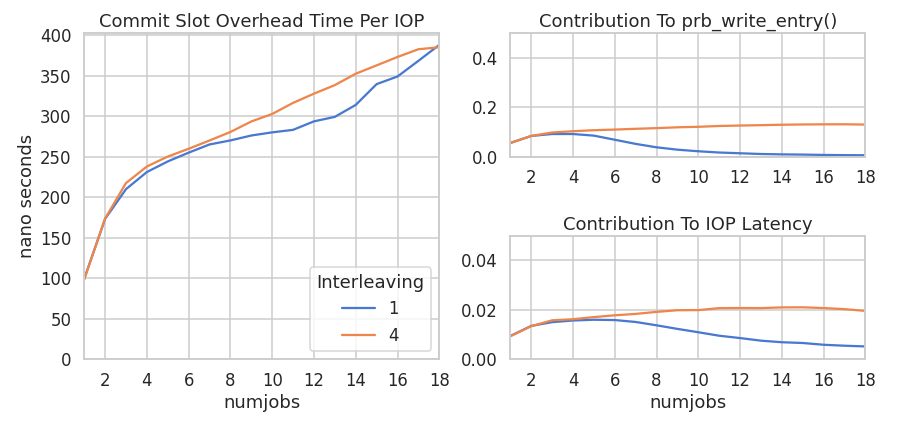
\includegraphics{fig/evaluation/ncommitters_scalability__overhead.pdf}
    \caption{
        Overhead of the \textit{commit slot} for $24 = {\texttt{\footnotesize ncommitters}} > \max numjobs$.
        Note the different y-axis scales.
        Also note that the relative latency contribution for the non-interleaved configuration only shrinks because the PMEM write time (not shown) grows significantly.}
    \label{fig:eval:ncommitters_scalability:overhead}
\end{figure}


We draw the following conclusions from our observations made above:
\begin{itemize}[noitemsep]
    \item The \textit{commit slot} mechanism successfully limits PMEM write time.
    \item The \textit{commit slot} mechanism's multi-core scalability is acceptable and contributes little relative overhead to each IOP compared to other ZFS components.
    \item Regarding the non-interleaved configuration (single Optane DIMM):
        \begin{itemize}
            \item Our 4k synchronous write workload is able to achieve peak performance with 400k IOPS as early as \lstinline{ncommitters=3}.
            \item Setting \lstinline{ncommitters=8} extends the peak to a plateau with regard to $numjobs$, but consumes $\frac{6.5~\text{us}}{3.3~\text{us}} = 1.96$ times more (on-CPU!) PMEM write time per IOP.
            \item Note that we used \lstinline{ncommitters=3} as the configuration for ZIL-PMEM in all of the previous benchmarks.
                Since our main evaluation system on which these benchmarks were executed only has 8 cores (2x SMT), this setting ensured CPU-efficient execution at all times.
                We believe that an efficiency-oriented default configuration is the preferable approach for an in-kernel filesystem such as ZFS which provides a system-wide OS service whose overall priority in the system is not known a priori.
                However, for systems whose primary role is that of an NFS/SMB server or that of a SCSI target (ZVOLs), it may be appropriate to allow more on-CPU waiting time.
        \end{itemize}
    \item Regarding the four-way interleaved configuration (4 Optane DIMMs):
        \begin{itemize}
            \item The \textit{commit slot} mechanism is not useful for the observed range of $numjobs$ values.
            \item The reason is that ZIL-PMEM cannot saturate the Optane DIMMs' write bandwidth due to per-IOP overhead added by other components of ZFS.
            \item However, with ${\texttt{\footnotesize ncommitters}} > \max numjobs$, the overhead per IOP is negligible.
        \end{itemize}
\end{itemize}

\chapter{Conclusion}\label{ch:conclusion}

We have demonstrated that the ZFS Intent Log~(ZIL), which is ZFS's mechanism for supporting synchronous IO semantics, is unable to take advantage of Persistent Memory (PMEM) as a \textit{separate log device} (SLOG).
Our analysis shows that the ZIL's block-device oriented data structure (LWB chain) as well as ZFS's IO abstraction (ZIO pipeline) add considerable latency overhead.
This observation motivated the development of ZIL-PMEM, our new ZIL implementation that exclusively targets PMEM.

In comparison to related work in academia, ZIL-PMEM falls into the category of an in-kernel cross-media filesystem that uses PMEM for acceleration of its write path.
Other publications in this niche are \textit{Ziggurat} and \textit{Strata} \cite{zhengZigguratTieredFile2019,kwonStrataCrossMedia2017}.
Ziggurat focuses on predictive data placement and can migrate data between different storage tiers such as PMEM and flash.
It is based on NOVA-Fortis and thus a PMEM-first design whereas ZIL-PMEM starts to introduce PMEM into a block-oriented system.
Strata uses PMEM as a log buffer for fast synchronous IO, and aggregates the log contents for efficient write-back to SSDs.
Its hybrid architecture (LD\_PRELOADed library + kernel module) is not directly comparable to ZIL-PMEM.
In the open source ecosystem, we have identified Linux Device Mapper with its \textit{dm-writecache} target as a practically relevant alternative to \mbox{ZIL-PMEM}.
Our survey of systems for modelling and/or validating filesystem crash consistency did not yield anything that would be directly applicable to our work with reasonable effort.
% we mention PMTest in future work

Our main contribution is the PRB/HDL data structure which consumes the space of a PMEM SLOG device and exposes the abstraction of per-dataset virtual, persistent, and garbage collected logs (HDLs).
PRB/HDL scales to many concurrent writers, is specifically optimized for Intel Optane PMEM's performance characteristics, and features an innovative mechanism to avoid excessive on-CPU waiting for PMEM IO.
To our knowledge, we are the first to identify and address this problem in the domain of PMEM-aware filesystems.
Our persistent data structure ensures data integrity through checksums and encodes logical dependencies between log entries in a way that allows for parallel writes to a HDL and yet results in a deterministic replay order during recovery.
The recovery procedure is crash-consistent and handles detected data corruption as well as \textit{machine check exceptions} (MCEs) correctly and gracefully.

We have integrated PRB/HDL into ZFS such that the old ZIL implementation (ZIL-LWB) and ZIL-PMEM can coexist at runtime.
Our approach shares the code and data structures that define the logical structure of the ZIL, but provides sufficient flexibility for different persistence mechanisms.
Whereas there are still open issues related to dynamic changing of ZIL kinds after pool creation, and the overall degree to which ZIL kinds should be exposed to the user, we were able to successfully evaluate our implementation.

We have validated correctness through extensive unit testing as well as existing ZIL tests in the ZFS Test Suite and the \textit{ztest} stress testing tool.
We achieve X\% code coverage for our userspace tests, and Y\% code coverage for the kernel module.\todo{code coverage results}
Regarding performance, we were able to demonstrate high speedups over ZIL-LWB in micro- and application benchmarks.
The highest achieved speedups are 8x (4k synchronous random write micro-benchmark) and 5.8x in a RocksDB workload.
The speedup of the same workloads for ZVOLs with XFS mounted on top is, barring a few exceptions, at least~2x.
In comparison to other block-oriented systems that were adapted to PMEM (Ext4 or XFS on PMEM or dm-writecache), ZFS with ZIL-PMEM performs exceptionally well for small synchronous operations (Redis, RocksDB), presumably due to lower write amplification.
% However, in all-PMEM configurations, the performance advantage of the Linux filesystems is still significant.
Our experimental \textit{ITXG bypass} for ZVOLs with which we sought to demonstrate the benefits of parallel logging to the same HDL showed some benefit in the micro-benchmark, but not in the application benchmarks.
Our \textit{commit slot} mechanism for avoidance of excessive on-CPU waiting when the maximum PMEM write bandwidth is exceeded was shown to be effective for a single non-interleaved Optane DIMM but is not practically relevant with four interleaved DIMMs at current CPU core counts.

\section{Future Work}\label{sec:futurework}

We would like to systematically \textbf{validate the speculations about write amplification} that we made in the evaluation.
This requires instrumentation of all benchmarked storage stacks.
The minimum required metrics are the sum of application data that were written at the VFS level, and the number of bytes written to PMEM.
Histograms for the distribution of the VFS and PMEM write sizes could also be useful to compare the degree to which aggregation of IO operations takes place in different storage stacks and workloads.
Whereas eBPF would work for this task, the measurement overhead is not negligible.
Statically compiled, low overhead, per-CPU counters are likely preferable.

ZIL-PMEM's \textbf{multi-core scalability for a single dataset} is significantly worse than in configurations with a dedicated dataset per parallel writer.
This can be observed by comparing the IOPS achieved by ZIL-PMEM in Figure~\ref{fig:eval:fio4k:metrics} (per-thread datasets) to \textit{fio-growing} in Figure~\ref{fig:eval:appbenchmarks:zilpmem_vs_zilllwb} (shared dataset).
Whereas the values for scaling factor (=\lstinline{numjobs}) 1 are expectably the same, \textit{fio-growing} only achieves approximately 50\% of the IOPS at \lstinline{numjobs=4} and \lstinline{8}.
For \lstinline{numjobs=4}, we believe that this is due to the use of a per-dataset mutex to ensure a sequential log structure (Section~\ref{sec:zilpmem:zilog}).
The effect does not grow further for \lstinline{numjobs=8} because we are already limited by PMEM bandwidth at \lstinline{numjobs=4}.
An extended latency breakdown that measures the time spent acquiring the per-dataset mutex could be used to confirm this hypothesis.

Our evaluation does not address the \textbf{performance of the recovery path}.
We expect the relevant factors to be a) the number of dataset in the pool, b) the chunk size, and c) the number of chunks.
The important metrics for recovery are a) pool import time, b) replay time, and c) peak aggregate DRAM usage by the per-HDL data structures.

The trade-offs around the \textbf{chunk size} have not yet been evaluated.
We chose a large chunk size for our evaluation (128 MiB) to avoid contention on the PRB-wide mutex that must be held while getting a new free chunk.
% For example, the 128 MiB chunk size allows for $\frac{128 * 2^20}{256 + 192 + 4*2^10 + (256 - 192)} \sim 30840$ 4k log entries per chunk.
% Consequently, only every ${30840^\text{th}}$ log entry would need to acquire the PRB-global mutex to get a new chunk.
Such a large chunk size is probably not required in practice.
For example, in a 4k write workload, only every $\frac{128 * 2^{20}}{256 + 192 + 4*2^{10} + (256 - 192)} \sim 30840^\text{th}$ write would require a new chunk, which assuming back-to-back writes at a very optimistic latency of 1.5~us, is only every 46.2~ms.
Since data corruption of an entry header makes the subsequent entries in the chunk unreachable for traversal, we expect that it is desirable to find the smallest possible chunk size that works on a given system.

We explicitly ignored \textbf{space efficiency} as a concern for ZIL-PMEM because of the high capacity of Intel Optane PMEM.
However, determining and potentially reducing the per-entry space overhead of ZIL-PMEM could be beneficial for media wear-out.
Users with NVDIMM-N devices, which are usable with ZIL-PMEM in principle but have DRAM-level capacities and significantly higher prices, could benefit as well.
Possible approaches to reduce space overhead are:
\begin{itemize}[noitemsep]
    \item Batching of multiple small log records into a single PRB entry (e.g., directory operations, file metadata).
    \item Reduction or omission of padding in the in-PMEM structure.
        Whereas padding to 256 byte multiples delivers the best performance on Optane PMEM, it is presumably unnecessary on DRAM/NVDIMM-N~\cite{yangEmpiricalGuideBehavior2020}.
\end{itemize}

We would like to \textbf{extend our performance evaluation} with the following storage stacks:
\begin{description}[noitemsep,leftmargin=1.5cm,labelindent=1cm]
    \item[ZIL ZIO Bypass By Saji Nair]
    At the OpenZFS 2020 Developer summit, Saji Nair of storage vendor Nutanix presented a proof-of-concept for handling fast block devices more efficiently when configured as SLOGs.
    The prototype avoids unnecessary sequential ordering of IO operations when writing LWBs.
    It also avoids using the ZIO pipeline due to context switching overheads and issues block IO directly from the application thread instead.
    The evaluation is limited to a single benchmark: a~fio~8k~(!) sync write workload, spread across four zpools in identical configuration, achieves 75k IOPS at four threads.
    With 16 threads, the system achieves its peak IOPS at approx. 125k IOPS.
    The source code for the prototype has not been published and the design is incomplete with regard to replay.~\cite{openzfsZILPerformanceImprovements2020}

    \item[Ext4 journal\_dev / XFS logdev] Both XFS and Ext4 provide an option to configure dedicated journaling / write-ahead logging devices.
        However, performance during manual experimentation with this feature was unexpectedly low for both filesystems.
        Since both configurations seem rather exotic, we ultimately did not use them in the evaluation.

    \item[XFS DAX Log Patch] XFS developer Christoph Hellwig has published an unfinished patch that adds DAX support for the code in XFS that writes its write-ahead log~\cite{LKMLChristophHellwig}.
        Our understanding of the patch is that it bypasses the block IO layer but leaves the persistent structure unchanged.
        The experiment would be particularly interesting in combination with a (properly tuned) dedicated logdev configuration for XFS.
\end{description}

Regarding \textbf{correctness and robustness} of our implementation, we would like to explore the following topics in the future:
\begin{description}[noitemsep,leftmargin=1.5cm,labelindent=1cm]
    \item[Validating PMEM Durability] PMTest is a tool which automatically validates that the software under test issues the architectually required instructions for durability (Section~\ref{sec:rel_work:pmemspecifictools}).
        In contrast to other tools, it supports kernel mode \textit{and} is publicly available.

    \item[Fault Injection for PMEM Access] Whereas we are careful to always use \lstinline{memcpy_mcsafe} when accessing PMEM, we do not have tests that verify the error handling path.
        As described in our literature review (Section~\ref{sec:rel_work:fault_injection}), fault injection is the tool of choice for such tests.
        Either \textit{ndctl-inject} or an extension of ZFS's existing fault injection infrastructure that intercepts PRB's PMEM access could be used.

    \item[Fuzzing] Fuzzing could potentially be used harden our implementation against unexpected in-PMEM state.
        Our software engineering efforts to facilitate testing of PRB/HDL might enable the use of established userspace tooling with reasonable effort.
\end{description}

Our implementation does not yet attempt to \textbf{detect write errors or unsafe shutdowns} (ref. Section~\ref{sec:background:pmemprogrammingmodel}).
The PRB garbage collection procedure presents is an opportune point for eager detection of media errors by traversing a chunk's content before garbage-collecting it.
If the PMEM hardware detects an error, the problem will be surfaced via an MCE and can be reported to the user.
As an end-to-end check, PRB further stores a checksum of a chunk's content in its DRAM representation. This checksum could be validated against the readable PMEM content during garbage collection.
Regarding unsafe shutdowns, it would be a good extension of the user experience to detect the condition and to surface it to the user via \lstinline{zpool status} or during pool import.
However, we believe that ZIL-PMEM's existing measures to detect data corruption should be able to correctly handle problems caused by unsafe shutdowns on the fly.

For the \textbf{integration into ZFS}, we anticipate the following future work items:
\begin{description}[noitemsep,leftmargin=1.5cm,labelindent=1cm]
    \item[PMEM Space Management] For maintainability and other use cases for PMEM in ZFS, it might be sensible to integrate PMEM allocation more deeply into the SPA.
        For example, the allocation interface could be extended such that it becomes possible to request DAX-capable blocks.
        Instead of our simplistic partitioning scheme for dividing the entire PMEM space into chunks (Section~\ref{sec:zilpmemzilkind:spacereservation}), ZIL-PMEM would pre-allocate chunks from the SPA and remember their DVA by storing them in the object set.

    \item[ZIL Kinds User Experience] The goal to make ZIL-PMEM, or ZIL kinds in general, fully transparent to the administrator should be reconsidered.
        (See Section~\ref{sec:zilpmemzilkind:activation} for our rationale.)

    \item[Support for Native Encryption] The threat model for supporting \mbox{OpenZFS} Native Encryption in ZIL-PMEM must be the same as for ZIL-LWB.
        The entry header and body need to be authenticated and the entry body needs to be encrypted.
        ZIL-PMEM's recovery path needs to be vetted to ensure that recorded entries cannot be injected into unintended replay sequences (replay attack).

    \item[Redundancy Through Mirroring] Redundancy in ZIL-PMEM could be achieved through mirroring of PRB between two or more DIMMs.
        During recovery, we would always scan both PRBs and deduplicate the discovered entries.
\end{description}

\backmatter

\chapter{Appendix}\label{ch:appendix}

\cleardoublepage
\phantomsection
\addcontentsline{toc}{chapter}{Bibliography}
\emergencystretch=1em
\printbibliography

\end{document}
